\documentclass[11pt]{amsart}
\usepackage[T1]{fontenc}
\usepackage{lmodern}
\input{glyphtounicode-cmex.tex}
\usepackage[margin=1in]{geometry}
\usepackage{amsmath,amssymb,amsthm,mathtools,mathrsfs}
\usepackage{microtype}
\usepackage{enumitem,booktabs,array,longtable,needspace}
\usepackage{graphicx,xcolor}
\usepackage{tikz}
\usetikzlibrary{arrows.meta,positioning,calc,fit}
\usepackage[colorlinks=true,linkcolor=blue!45!black,citecolor=green!35!black,urlcolor=blue!55!black]{hyperref}
\hypersetup{pdftitle={Deforming hypersymplectic four-manifolds to hyperkahler triples},pdfauthor={OpenAI},pdfsubject={Hypersymplectic deformation in fixed cohomology classes}}
\usepackage[capitalise,nameinlink,noabbrev]{cleveref}
\numberwithin{equation}{section}
\theoremstyle{plain}
\newtheorem{theorem}{Theorem}[section]
\newtheorem{lemma}[theorem]{Lemma}
\newtheorem{proposition}[theorem]{Proposition}
\newtheorem{corollary}[theorem]{Corollary}
\theoremstyle{definition}
\newtheorem{definition}[theorem]{Definition}
\newtheorem{notation}[theorem]{Notation}
\theoremstyle{remark}
\newtheorem{remark}[theorem]{Remark}
\newcommand{\R}{\mathbb R}
\newcommand{\C}{\mathbb C}
\newcommand{\Z}{\mathbb Z}
\newcommand{\Q}{\mathbb Q}
\newcommand{\N}{\mathbb N}
\newcommand{\dd}{\mathrm d}
\newcommand{\eps}{\varepsilon}
\DeclareMathOperator{\Id}{Id}
\DeclareMathOperator{\dist}{dist}
\DeclareMathOperator{\supp}{supp}
\DeclareMathOperator{\spt}{spt}
\DeclareMathOperator{\vol}{vol}
\DeclareMathOperator{\rank}{rank}
\DeclareMathOperator{\tr}{tr}
\DeclareMathOperator{\Pic}{Pic}
\DeclareMathOperator{\PD}{PD}
\DeclareMathOperator{\im}{im}
\DeclareMathOperator{\sgn}{sgn}
\setlist{itemsep=3pt,topsep=5pt}
\setcounter{tocdepth}{1}
\emergencystretch=1.5em

\title[Deforming hypersymplectic four-manifolds]{Deforming hypersymplectic four-manifolds to hyperk\"ahler triples}
\author{OpenAI}
\date{September 23, 2026}
\begin{document}
\begin{abstract}
Every smooth normalized positive triple of closed two-forms on a closed
connected oriented four-manifold admits a smooth deformation, with each
cohomology class fixed, to a hyperk\"ahler triple.
This resolves Donaldson's hypersymplectic deformation conjecture.
\end{abstract}
\maketitle
\section{Introduction}\label{sec:introduction}

A \emph{hypersymplectic structure} on an oriented four-manifold is a triple
of closed real two-forms whose pointwise span is three-dimensional and
positive definite for the wedge product. Such a triple determines a conformal structure,
but its forms need not be parallel. After a constant normalization of
their intersection matrix, the question is whether one can deform the
forms to a hyperk\"ahler triple while retaining their three cohomology
classes.

\begin{theorem}\label{thm:main}
Let $X$ be a closed connected oriented smooth four-manifold, and let
$\omega=(\omega_1,\omega_2,\omega_3)$ be a smooth hypersymplectic structure
normalized by
\begin{equation}\label{eq:intro-normalization}
 \int_X\omega_i\wedge\omega_j=\delta_{ij}.
\end{equation}
There is a smooth family of hypersymplectic structures $\omega(t)$,
$0\le t\le1$, such that
\[
 \omega(0)=\omega,\qquad [\omega_i(t)]=[\omega_i]
 \quad (i=1,2,3),
\]
and a positive volume form $\mu_1$ with
\begin{equation}\label{eq:intro-endpoint}
 \omega_i(1)\wedge\omega_j(1)=2\delta_{ij}\mu_1.
\end{equation}
The endpoint forms are parallel and self-dual for a hyperk\"ahler metric.
\end{theorem}

For an arbitrary positive volume form $\mu$, write
$\omega_i\wedge\omega_j=2\mathcal Q_{ij}\mu$. There is a unique choice
of $\mu$ for which $\det\mathcal Q=1$, and
\eqref{eq:intro-endpoint} is exactly $\mathcal Q=I_3$ in this convention.
The statement is unaffected by a constant orthogonal change of the
ordered triple.

The normalization also specifies the conclusion for any initial positive
closed triple. Let $G_{ij}=\int_X\omega_i\wedge\omega_j$; this matrix is
positive definite. Choose a constant invertible real matrix $L$ with
$LGL^{\mathsf T}=I_3$ and apply \Cref{thm:main} to $L\omega$.
Applying $L^{-1}$ to the resulting path preserves positivity and each
original class. Its endpoint satisfies
\[
 \omega_i(1)\wedge\omega_j(1)=2G_{ij}\mu_1,
\]
where $\mu_1$ is the volume form of the normalized endpoint metric.
Thus the original basis consists of parallel self-dual forms for a
hyperk\"ahler metric, with its original Gram matrix $G$.

\begin{corollary}[Individual K\"ahler realizations]\label{cor:individual-kahler}
Let $X$ be a closed connected oriented smooth four-manifold with a smooth
positive triple $\omega$ of closed real two-forms. For every fixed
$c\in\mathbb R^3\setminus\{0\}$, the form $\alpha_c=\sum_i c_i\omega_i$
is a K\"ahler form for a parallel integrable complex structure $J_c$ of
some hyperk\"ahler metric $g_c$ on $X$:
\[
 \alpha_c(v,w)=g_c(J_cv,w).
\]
The compatible structure is chosen separately for each $c$; no simultaneous
transport of the triple is asserted.
\end{corollary}
\begin{proof}
Use the fixed-class path for the original basis described above and put
$\alpha_t=\sum_i c_i\omega_i(t)$. Positivity of the pointwise wedge-product
matrix gives $\alpha_t\wedge\alpha_t>0$. Thus $\alpha_t$ is symplectic,
and its class is fixed because each $[\omega_i(t)]$ is fixed.

For the endpoint metric $g$, set $r_c=(c^{\mathsf T}Gc)^{1/2}>0$.
The endpoint identities show that $\alpha_1/r_c$ is parallel and self-dual
with $g$-norm $\sqrt2$. It therefore defines a parallel integrable complex
structure $J^{\mathrm{end}}_c$ with
$\alpha_1/r_c=g(J^{\mathrm{end}}_c\,\cdot,\cdot)$.
Hence $\alpha_1$ is its K\"ahler form for the hyperk\"ahler metric $r_cg$.

Since $X$ is closed, Moser's theorem gives an isotopy $\phi_{c,t}$ with
$\phi_{c,0}=\mathrm{id}$ and $\phi_{c,t}^*\alpha_t=\alpha_c$.
Pulling back $r_cg$ and $J^{\mathrm{end}}_c$ by $\phi_{c,1}$ gives the
claimed hyperk\"ahler metric and compatible integrable structure on $X$.
Fine and Yao note this Moser implication for a constituent in
\cite[Section~1]{FineYao2017}.
\end{proof}

\begin{corollary}[Smooth type]\label{cor:smooth-type}
Let $X$ be a closed connected smooth four-manifold admitting a smooth
positive triple of closed real two-forms. Then $X$ is diffeomorphic to
the standard K3 manifold or to $T^4$.
\end{corollary}
\begin{proof}
Give $X$ the orientation induced by the triple. The normalization above
and \Cref{thm:main} give a global hyperk\"ahler triple on $X$. Choosing
one of its complex structures makes $X$ a compact K\"ahler surface with
a nowhere-vanishing holomorphic two-form. The compact hyperk\"ahler
surface classification \cite[Section~2, p.~162]{Boyer1988} therefore
identifies $X$ itself as a complex two-torus or a K3 surface. A complex
two-torus is smoothly $T^4$, while every complex K3 surface is
diffeomorphic to a nonsingular quartic surface in $\mathbf P^3$, the
standard K3 manifold \cite[p.~58]{Kodaira1970}.
\end{proof}

\subsection{History and significance}

Donaldson's study of closed two-forms on four-manifolds links their
pointwise wedge-product geometry to nonlinear elliptic equations
\cite{Donaldson2006}. His Question~3 in Section~5.3 asks whether a
compact oriented four-manifold carrying a positive closed triple
admits a hyperk\"ahler structure. In the same section he proposes a
prescribed-volume continuity argument in the simply connected case,
conditional on a priori estimates and an auxiliary involution. The
involution keeps the evolving form in a fixed cohomology class
\cite[Section~5.3]{Donaldson2006}.
Fine and Yao formulate the normalized
deformation problem, retaining all three cohomology classes, as
Conjecture~1.1 of \cite{FineYao2017}.
\Cref{thm:main} resolves this deformation conjecture positively.
Keeping the classes connects the given triple to a metric with its
prescribed periods, beyond existence of some hyperk\"ahler metric on
the same manifold.

The main analytic approach has been the hypersymplectic flow.
Fine and Yao obtained this flow by reducing the $G_2$-Laplacian flow
on the product with a three-torus. They proved that a finite-time
solution extends while the associated seven-dimensional scalar
curvature, equivalently the torsion, remains bounded
\cite[Theorem~1.3]{FineYao2017}. Their later work gives an integral
torsion extension criterion, global existence near pointwise
orthogonality, and subsequential convergence of global solutions under
additional geometric bounds
\cite[Theorems~4.7, 4.10, 4.15 and~4.16]{FineYao2020}.

Several restricted classes admit complete convergence results.
Huang, Wang and Yao proved convergence, after pullback by
diffeomorphisms, for simple-type hypersymplectic structures on
the standard four-torus, a diagonal one-variable class
\cite[Theorems~3.5 and~3.6]{HuangWangYao2018}.
Picard and Suan treated $G_2$ flows associated with K\"ahler
Calabi--Yau data; their complex-dimension-two case supplies a
hypersymplectic convergence theorem
\cite[Theorem~1.3]{PicardSuan2024}.
Fine, He and Yao extended the simple-type convergence result, modulo
diffeomorphisms, to
$T^3$-invariant triples on $T^4$ in symmetric normal form
\cite[Theorem~1.5]{FineHeYao2024}. They subsequently proved
a linear cohomologous isotopy to a hyperk\"ahler triple when an
effective smooth circle action preserves the initial triple
\cite[Theorem~1.2]{FineHeYao2025}.
Related reductions and coflow constructions appear in work of Petcu,
Yao and Zhou, and Karigiannis, Picard and Suan
\cite{Petcu2026,YaoZhou2026,KarigiannisPicardSuan2026}.
These results retain their stated symmetry or integrability hypotheses.
The path constructed here starts from an arbitrary positive closed
triple; its existence is a separate question from convergence or
uniqueness for the hypersymplectic flow.

The topology already places strong restrictions on such a triple.
Any two of its forms determine an almost-complex structure whose
canonical line is trivial, and the third form tames that structure.
Here a real two-form $\beta$ \emph{tames} $J$ if
$\beta(v,Jv)>0$ for every nonzero vector $v$; it is
\emph{compatible} if it is also $J$-invariant. A closed tamer is
symplectic. Bauer's bound for symplectic four-manifolds with torsion
first Chern class \cite[Corollary~1.2]{Bauer2008}, together with the
three positive period classes, gives $b^+=3$, where $b^+$ is the
positive index of the intersection form. The resulting free
intersection lattice is the K3 lattice or three hyperbolic planes.
These facts supply the lattice used below; they do not presuppose a
smooth identification of the initial manifold with a K3 surface or torus.

For controlling closed positive forms, Sullivan's structure currents
provide the cone-duality framework \cite{Sullivan1976}.
Harvey and Lawson developed the positive-current characterization of
K\"ahler geometry \cite{HarveyLawson1983}, and Li and Zhang compared
the taming and compatible cones in almost-complex geometry
assuming the compatible cone is nonempty \cite{LiZhang2009}.
A separate article proves that every tamed smooth
almost-complex structure on a closed connected real four-manifold admits a compatible
symplectic form \cite[Theorem~1.1]{OpenAITaming2026}. Its current
estimates and density-splitting argument are also used here, with the
needed proofs included in \Cref{sec:current-energy,sec:density-splitting}.
In particular, smooth density-weight closedness already appears in
the proof in Section~6 of that article. Its compatible class is
unrestricted. The additional class criterion below converts closed
normalized density thresholds into curves, using Preiss's
rectifiability theorem and Rivi\`ere--Tian's regularity theorem for
integral cycles \cite{Preiss1987,RiviereTian2009}. This supplies the
prescribed taming class needed along the deformation.

\subsection{The main ideas}

The proof organizes the deformation around a pair of forms. Write an
ordered triple as $(A,C,B)$, and write products of forms for wedge
products. The positive plane spanned by $A,C$
determines an almost-complex structure $J$, with sign chosen so that
$B$ tames it. A pair deformation gives the desired triple deformation
provided the original third class continues to contain a tamer.
The argument first proves a criterion for this availability, then
constructs a fibration and an auxiliary equal-square pair, and finally
uses two classical K\"ahler steps to reach the endpoint.

\paragraph{Currents and a prescribed class.}
Separation of the cone of positive forms gives a positive current
obstructing a desired closed form. Quadratic mass estimates bound its
mass in a ball of radius $r$ by $Kr^2$ for a fixed constant $K$.
Resolvent regularization also
controls how its complex-line directions vary on that scale.
Together these estimates prove closedness after weighting by smooth
functions of the two-dimensional density. The zero-density part can
then be handled by the intersection form, while normalized thresholds
of the positive-density part give integral pseudoholomorphic cycles.
Compatibility is proved before the integral-cycle regularity theorem
is applied, so that its local symplectic hypothesis is available.

The output is \Cref{thm:tamed-compatible,thm:taming-cone}.
For the second theorem, let $V$ be the intersection-orthogonal
complement of $[A],[C]$. It has Lorentz signature because $b^+=3$.
A positive-square class $H\in V$ is a taming class if it is in the
same positive component as a known positive-square taming class $U\in V$ and
pairs positively with every irreducible closed $J$-curve. The
criterion will keep $[B]$ available as the pair changes.

\paragraph{Marked curves and a torus fibration.}
The initial triple supplies an entire coefficient sphere of
almost-complex structures: for $v\in S^2$, the forms
$a\cdot\omega$ with $a\cdot v=0$ constitute its anti-invariant plane
(a form $\xi$ is anti-invariant when $\xi(Ju,Jw)=-\xi(u,w)$),
and $v\cdot\omega$ tames the
corresponding structure. Compatible forms can be selected smoothly
over this sphere by a constant-rank elliptic correction. After projecting
their classes to the original positive period plane and normalizing,
one obtains a degree-one map to its unit sphere.
Li proposed using such winding sphere families, parametrized wall crossing,
and Taubes's curve correspondence to construct elliptic fibrations
\cite[Section~7.4.1]{Li2010SCY}. The marked-family construction below
carries out this approach for the coefficient sphere of the initial triple.
Li--Liu's families wall-crossing and index formulas
\cite{LiLiu2001}, together with Taubes's canonical nonvanishing and
large-parameter curve extraction
\cite{Taubes1994,Taubes1996,Taubes1999}, then give curves through every
point in a chosen nonzero integral square-zero class.
To impose passage through a chosen point, the proof requires one
component of the Seiberg--Witten spinor to vanish there. As the parameter moves
over the sphere, the line containing that component also varies and
has degree of absolute value one. Its contribution must be retained
in the marked wall-crossing calculation, even though the underlying
Spin-c structure is fixed throughout the family.

The integral class is chosen to prevent any such curve configuration
from splitting. Eichler's criterion supplies the lattice normal form
\cite[Proposition~3.3(i)]{GritsenkoHulekSankaran2009}; a further
finite-coset argument works for the arbitrary real positive period
plane of the original triple. Pseudoholomorphic adjunction and
positivity of intersections then reduce the possible fibers to tori
and rational curves with one singularity
\cite{McDuffSalamon2012,Wendl2020}.
To obtain ordinary nodes, we prove transversality using exact
perturbations of $A,C$ with $B$ fixed. The first-jet method is related
to that of Oh and Zhu \cite{OhZhu2008}, but the allowable closed-form
variations require their own cokernel calculation. Relative nodal
replacement and local deformation theory now produce the fibration
of \Cref{thm:pencil}: a proper map from $X$ to a closed oriented
surface, with torus regular fibers and rational singular fibers having
one ordinary node.

\paragraph{An auxiliary volume equation.}
The fibration supplies classes with small positive fiber area.
Near a nodal fiber we use the Gibbons--Hawking construction
\cite{GibbonsHawking1978} and the periodic Ooguri--Vafa model
\cite{OoguriVafa1996}. Gross and Wilson developed the corresponding
mathematical collapsing and semi-flat gluing methods for elliptic
K3 surfaces \cite{GrossWilson2000}. Here the nodal holomorphic model
is constructed independently, since a global complex structure is
not yet available. On fixed annuli the model and regular data agree
up to exponentially small error. Matching the fiber area and the
period on the surface swept out by the monodromy-invariant fiber
cycle ensures that the discrepancy has a primitive.

After exact preparation of the pair, these local forms glue to an
approximate auxiliary form of fiber area $\epsilon$.
The correction in \Cref{thm:auxiliary-solution} is solved on exact
two-forms. For any Riemannian metric on the oriented closed four-manifold, let
$h^+$ denote the self-dual part of an exact two-form $h$. The exact-form
identity used in Donaldson's elliptic formulation
\cite[Section~2, proof of Proposition~1; Section~4, Lemma~1]{Donaldson2006}
\[
 \|h\|_{L^2}^2=2\|h^+\|_{L^2}^2\qquad(h\text{ exact})
\]
controls the inverse while the fibers collapse. The remaining finite
Sobolev estimates lose only powers of $\epsilon^{-1}$, which are
absorbed by the exponentially small gluing error. This produces a
closed form $D$ satisfying $AD=CD=0$ and $D^2=A^2$.
The class inequality in \Cref{prop:auxiliary-class} holds for all
later curves at one fixed choice of $\epsilon$; it transfers
positivity from $[D]$ to the original class $[B]$.

\paragraph{Two K\"ahler steps in the original classes.}
The closed equal-square pair $A,D$ defines an integrable complex
structure with holomorphic two-form $A\pm iD$, choosing the sign
so that $C$ tames it. The compact-surface
criteria of Buchdahl and Lamari, and the numerical K\"ahler-cone
criterion, put $[C]$ in the K\"ahler cone
\cite{Buchdahl1999,Lamari1999,DemaillyPaun2004}.
Yau's volume theorem \cite{Yau1978} gives $C_1\in[C]$ with
$C_1^2=A^2$. Interpolate from $C$ to $C_1$; the uniform class
inequality and the taming criterion keep $[B]$ available throughout.
The pair $A,C_1$ is now itself an integrable equal-square pair.
A second K\"ahler step in $[B]$ gives $B_1$, completing the
hyperk\"ahler triple. Smooth selection of the third forms, with both
endpoints prescribed, gives the actual path $(A,C_t,B_t)$ shown in
\Cref{fig:endpoint-path}. Every component retains its original class.

\subsection{Organization and conventions}

\Cref{sec:definite-pairs} establishes the preliminary geometry and
topology. The positive-current results occupy
\Cref{sec:current-energy,sec:density-splitting}.
\Cref{sec:families,sec:lattice-chamber,sec:pencil} construct the
torus fibration, and
\Cref{sec:local-models,sec:regular-preparation,sec:auxiliary-volume}
construct the auxiliary equal-square pair. The proof of
\Cref{thm:main} is completed in \Cref{sec:endpoint}.

We write products of two-forms for wedge products and products of
degree-two cohomology classes for their intersection pairing.
Curve classes are identified with their Poincar\'e duals in cohomology.
Integral lattice statements use
\[
 \Lambda=H^2(X;\Z)/\operatorname{torsion}.
\]
The original positive period plane is
$P=\operatorname{span}\{[\omega_1],[\omega_2],[\omega_3]\}$.
No rationality of this plane is assumed. All deformations of forms are
smooth in the manifold variable; parameter regularity is stated where
it is used. Constants in local estimates may depend on fixed smooth
background data and on the indicated finite differentiation order.

\tableofcontents
\section{Definite pairs and the coefficient sphere}\label{sec:definite-pairs}

We first associate an almost-complex structure to a definite pair and
identify the condition on a third form that makes the triple positive.
This converts the later deformation problem into the choice of taming
forms in a prescribed class. We also establish the topological
restrictions and the degree-one sphere of structures needed to produce
curves in \Cref{sec:families}.

\begin{definition}
A pair $(A,C)$ of real two-forms is \emph{definite} if its wedge-product
matrix is positive definite at every point. A two-form $B$ \emph{tames}
an almost-complex structure $J$ if $B(v,Jv)>0$ for every nonzero tangent
vector $v$. It is \emph{compatible} if, in addition,
$B(Ju,Jv)=B(u,v)$. When these forms are called symplectic, closedness is
included.
\end{definition}

\begin{lemma}\label{lem:definite-pair}
A definite pair $(A,C)$ on an oriented four-manifold determines an
almost-complex structure up to sign. Its anti-invariant real two-form
bundle is pointwise spanned by $A,C$, and its canonical complex line
bundle is trivial. A third form $B$ completes a positive triple if and
only if it tames one of the two signs of this almost-complex structure.
On a connected manifold the sign is fixed by $B$.

A real two-plane is Lagrangian for both $A$ and $C$ if and only if it is
a complex line, without specifying its orientation.
\end{lemma}

\begin{proof}
Ratios of positive four-forms are smooth functions. Set
\begin{equation}\label{eq:pair-normalization}
 x=\frac{AC}{A^2},\qquad
 y=\left(\frac{C^2}{A^2}-x^2\right)^{1/2}>0,\qquad
 T=\frac{C-xA}{y}.
\end{equation}
Then $AT=0$ and $T^2=A^2>0$. Consequently
\[
 \Omega=A+iT,\qquad \Omega^2=0,\qquad
 \Omega\overline\Omega=2A^2>0.
\]
The form $\Omega$ is complex decomposable and its kernel in the
complexified tangent bundle is complementary to its conjugate. Taking
this kernel as $T^{0,1}$ defines an almost-complex structure with the
given orientation. Replacing $y$ by $-y$ conjugates $\Omega$ and changes
$J$ to $-J$. The real and imaginary parts of $\Omega$ span the
anti-invariant forms, and $\Omega$ is a nowhere-zero section of the
canonical bundle.

Choose any Hermitian metric for $J$. The invariant two-forms are the
wedge-orthogonal complement of $\operatorname{span}(A,C)$ and have
signature $(1,3)$. For the decomposition
$B=B^{1,1}+B^{2,0+0,2}$, the positive-triple condition is exactly
$(B^{1,1})^2>0$. A real $(1,1)$ form in complex dimension two has positive
square precisely when its two Hermitian eigenvalues have the same
strict sign. The positive component is the cone of forms positive on
every complex line. The anti-invariant summand vanishes on such lines,
so this is equivalent to taming by $B$. The other component is positive
for $-J$. Connectedness fixes the choice continuously and globally.

Finally, for independent real vectors $u,v$,
$A(u,v)=C(u,v)=0$ is equivalent to $\Omega(u,v)=0$.
In a complex two-dimensional vector space with a nondegenerate complex
volume form, this says that $u,v$ are complex dependent, equivalently
that their real span is a complex line.
\end{proof}

In particular, for fixed $J$ the space of taming two-forms is an open
convex cone. Its intersection with the closed representatives of any
one class is also convex. The associated notion of positivity will
always use the sign of $J$ fixed by a stated tamer.

\begin{proposition}\label{prop:topology}
If $X$ carries a positive closed triple, then
\[
 b^+(X)=3,\qquad
 (b_1(X),b^-(X))=(0,19)\ \text{or}\ (4,3).
\]
The free integral intersection lattice is respectively
$3H\oplus2(-E_8)$ or $3H$, where $H$ is the hyperbolic plane.
Every almost-complex structure obtained from a definite pair in the
triple has vanishing integral first Chern class.
\end{proposition}

\begin{proof}
By \Cref{lem:definite-pair}, one member of the triple is a symplectic
form taming an almost-complex structure whose canonical bundle is
trivial. The first Chern class of this symplectic form therefore
vanishes: the space of its tamed almost-complex structures is
contractible and contains compatible structures. Bauer's bound for a
closed symplectic four-manifold with torsion first Chern class gives
$b^+\le3$ \cite[Corollary~1.2]{Bauer2008}. The three independent
positive cohomology classes give the reverse inequality.

The characteristic-number identity $c_1^2=2\chi+3\sigma$, obtained
from $p_1=c_1^2-2c_2$, the Euler-number identity and the signature
theorem \cite[Corollaries~11.12 and~15.5, Theorem~19.4]{MilnorStasheff1974},
together with $b^+=3$, gives
\[
 0=19-4b_1-b^-,\qquad \sigma=4b_1-16.
\]
Moreover $w_2\equiv c_1=0\pmod2$, so $X$ is spin
\cite[Problem~14-B]{MilnorStasheff1974}. Rokhlin's theorem makes
$\sigma$ divisible by $16$ \cite{Rokhlin1952}.
Since $b^-\ge0$, these relations give
$b_1\in\{0,4\}$ and the displayed alternatives. Poincar\'e duality
makes the free intersection form unimodular, and the Wu formula makes
it even \cite[Theorem~11.14]{MilnorStasheff1974}. Classification of
indefinite even unimodular lattices now gives the two stated forms
\cite[Chapter~V, Section~2.2, Theorems~5--6]{Serre1973}.
Only the intersection lattice has been classified at this stage.
\end{proof}

The positive three-plane bundle spanned by the triple is the
self-dual bundle of a unique oriented conformal structure. Choose one
metric $g_0$ in that conformal class. Since the original forms are
closed and self-dual, they are harmonic, and
\begin{equation}\label{eq:pair-harmonic-basis}
 \mathcal H^+_{g_0}
 =\operatorname{span}_{\R}\{\omega_1,\omega_2,\omega_3\}
\end{equation}
by \Cref{prop:topology}. Here the span is the vector space of global
forms, with constant coefficients.

For $v\in S^2\subset\R^3$, let $B_v=v\cdot\omega$ and let
$\mathcal A_v$ be the plane of forms $a\cdot\omega$ with $a\perp v$.
Choosing the sign tamed by $B_v$ defines an almost-complex structure
$J_v$. This construction uses the plane $\mathcal A_v$ itself and does
not require a global choice of its ordered basis over $S^2$.

\begin{lemma}\label{lem:twistor-degree}
The family $J_v$ is smooth and is Hermitian for $g_0$. At every point
of $X$ its map to the twistor sphere has degree of absolute value one.
The closed $J_v$-anti-invariant forms form the two-dimensional space
$\mathcal A_v$.
\end{lemma}

\begin{proof}
The first assertion follows from the construction and the
self-dual description of Hermitian almost-complex structures in
dimension four. At a fixed point, let $K$ be the positive Gram matrix
of the triple for $g_0$. A vector normal to the coefficient plane
$v^\perp$, for this Gram matrix, has coefficients $K^{-1}v$.
Its pairing with $B_v$ is positive. Thus, after normalization, the
fundamental forms give the map
\[
 v\longmapsto\frac{K^{-1}v}{|K^{-1}v|}
\]
in radial coefficient coordinates. Positive definite matrices connect to the
identity through positive definite matrices, so this map has degree
one. The orientation convention identifying coefficient and twistor
spheres can change only its sign.

A closed anti-invariant form is self-dual for $g_0$, hence harmonic.
By \eqref{eq:pair-harmonic-basis} it is a constant combination of the
original triple. It is anti-invariant for $J_v$ exactly when that
coefficient vector lies in $v^\perp$. This proves the final assertion.
\end{proof}

After a constant orthogonal change of coefficients we will denote a
chosen original ordered triple by $(A,C,B)$. For all later exact
deformations of the pair, set
\begin{equation}\label{eq:pair-lorentz-space}
 V=[A]^\perp\cap[C]^\perp\subset H^2(X;\R).
\end{equation}
This space has signature $(1,b^-)$, and $[B]\in V$ is a unit timelike
vector. It determines the future component of the timelike cone.

\begin{lemma}\label{lem:complex-symplectic}
Let $A,D$ be closed real two-forms with
$AD=0$ and $A^2=D^2>0$ pointwise. Then $A+iD$ defines an integrable
complex structure, and is a nowhere-zero holomorphic two-form for it.
If a closed third form $C$ has $AC=DC=0$ and $C^2=A^2$, then the
resulting triple is hyperk\"ahler, after choosing the sign of the
complex structure so that $C$ is positive.
\end{lemma}

\begin{proof}
Set $\Omega=A+iD$ and use its kernel as $T^{0,1}$ as in
\Cref{lem:definite-pair}. For vector fields $U,V$ in that kernel,
Cartan's formula and $\dd\Omega=0$ give
\[
 \mathcal L_U\Omega=0,\qquad
 \iota_{[U,V]}\Omega
 =\mathcal L_U(\iota_V\Omega)-\iota_V(\mathcal L_U\Omega)=0.
\]
The kernel is involutive. The smooth Newlander--Nirenberg theorem
therefore gives integrability \cite{NewlanderNirenberg1957}, and
closedness of the $(2,0)$ form
$\Omega$ gives holomorphicity.

Under the additional assumptions, $C$ is a positive closed $(1,1)$
form, hence a K\"ahler form. Its metric volume is $C^2/2=A^2/2$.
The ratio $\Omega\overline\Omega/C^2$ is constant, so the holomorphic
volume form has constant pointwise norm. The Chern connection of the
canonical line then makes $\Omega$ parallel. For a K\"ahler metric
this is the connection induced by the Levi-Civita connection.
Thus $A,D,C$ are parallel; their normalized self-dual algebra gives
the hyperk\"ahler structure. Explicitly, if
$(\eta_1,\eta_2,\eta_3)=(A,D,C)$ and $\mu=A^2/2$, then
$\eta_i\wedge\eta_j=2\delta_{ij}\mu$; thus their normalized
matrix $\mathcal Q$ from the introduction is the identity.
\end{proof}

\section{Separation, quadratic mass, and angular energy}
\label{sec:current-energy}

The two separation arguments below produce a positive current, possibly with
an anti-invariant correction.  We first control its trace measure at the
two-dimensional scale.  An intersection pairing then controls the correction
and the variation of the complex-line directions.  These estimates will
permit the density decomposition in \Cref{sec:density-splitting}.

Separation by positive currents follows the framework of Sullivan and
Harvey--Lawson \cite{Sullivan1976,HarveyLawson1983}, with the
almost-complex formulation of Li--Zhang
\cite[Section~3]{LiZhang2009}. The closed lift,
quadratic mass estimate and resolvent argument also occur in
\emph{Taming implies compatibility on four-manifolds}
\cite[Sections~2--4]{OpenAITaming2026}. We develop the estimates for
both separators together. In the prescribed-class application, the
closed current can have nonzero cohomology class, and its square must
remain in the energy identity.

\subsection{Conventions and separation}

Fix a smooth almost-complex structure $J$ on the closed four-manifold $X$,
give $X$ its complex orientation, and choose a smooth $J$-Hermitian metric
$g$.  Its fundamental form is
\[
 G(u,v)=g(Ju,v).
\]
The pointwise orthogonal decomposition is
\begin{equation}\label{eq:current-bundles}
 \Lambda^2=I\oplus E,
 \qquad I=\Lambda_J^+=\R G\oplus\Lambda_g^-,
 \qquad E=\Lambda_J^-\subset\Lambda_g^+.
\end{equation}
Let $R$ denote the orthogonal projection onto $E$.  A unit complex-line
bivector is $\ell=e\wedge Je$, where $|e|_g=1$.  We use $g$ to identify
bivectors and two-forms.  Consequently
\begin{equation}\label{eq:current-line-normalization}
 |\ell|_g=1,\qquad \ell^+=G/2,\qquad G(\ell)=1,
 \qquad |G|_g^2=2.
\end{equation}
The bundle of these bivectors is denoted by $\mathcal L\longrightarrow X$.

A two-current is a continuous real linear functional on
$\Omega^2(X)=C^\infty(X,\Lambda^2)$.  Under the metric identification its
coefficient is a distributional two-form, denoted by the same letter:
$T(\xi)=\langle T,\xi\rangle$.  Thus
\begin{equation}\label{eq:current-dual-convention}
 T\text{ is closed}\ \Longleftrightarrow\
 T(\dd\alpha)=0\text{ for all }\alpha\in\Omega^1(X)
 \ \Longleftrightarrow\ \dd^*T=0
 \ \Longleftrightarrow\ \dd(*T)=0.
\end{equation}
The cohomology class dual to a closed current is $[*T]\in H^2(X;\R)$.
For smooth coefficients this convention gives
$T(\xi)=\int_X\xi\wedge *T$.  Inner products between $L^2$ coefficients
will be written $\langle\ ,\ \rangle_2$.

Let
\[
 \mathcal P_J=\{\xi\in\Omega^2(X):\xi(\ell)>0
                    \text{ for every }\ell\in\mathcal L\},
 \qquad
 \mathcal Z_J=\{\xi\in C^\infty(X,I):\dd\xi=0\}.
\]
The set $\mathcal P_J$ is an open convex cone in the smooth topology;
openness already holds in the uniform topology.  Its closed elements are
precisely the symplectic forms taming $J$.  The elements of
$\mathcal P_J\cap\mathcal Z_J$ are the compatible symplectic forms.

\begin{lemma}[The two separators]\label{lem:current-separators}
The following statements hold.
\begin{enumerate}[label=\textup{(\roman*)}]
\item If $\mathcal P_J\cap\mathcal Z_J$ is empty, there is a nonzero current
 $N$ which annihilates $\mathcal Z_J$ and all anti-invariant forms, and is
 nonnegative on semipositive invariant forms.
\item If $H\in H^2(X;\R)$ has no representative in $\mathcal P_J$, there
 is a nonzero positive invariant current $N$ which is closed and satisfies
 $N(H)\le0$.
\end{enumerate}
In either case one can normalize $N(G)=1$ and choose a positive Borel
measure $\lambda$ on $\mathcal L$ such that
\begin{equation}\label{eq:current-line-measure}
 N(\xi)=\int_{\mathcal L}\xi_y(\ell)\,\dd\lambda(y,\ell),
 \qquad \mu=(\operatorname{pr}_X)_*\lambda,
 \qquad \mu(X)=1.
\end{equation}
In particular $N$ has order zero and belongs to $H^{-3}(X,\Lambda^2)$.
\end{lemma}

\begin{proof}
For \textup{(i)}, apply separation of an open convex set and a disjoint
linear subspace in the real locally convex space $C^\infty(X,I)$.
The separating continuous functional vanishes on $\mathcal Z_J$ and is
nonnegative on its positive cone.  Extend it to all two-forms by
precomposing with $1-R$.  Adding a positive multiple of $G$ and taking
a limit proves nonnegativity on every semipositive invariant form.

For \textup{(ii)}, choose a smooth closed representative $\beta$ of $H$
and separate the open cone $\mathcal P_J$ from the affine subspace
$\beta+\dd\Omega^1(X)$ in $\Omega^2(X)$.  If $N$ is the separating
functional, the unbounded translation directions in this affine subspace
give $N(\dd\alpha)=0$.  Every positive form can be multiplied by any
positive scalar, so the separation inequalities imply both
$N(\mathcal P_J)\ge0$ and $N(\beta)\le0$.  Adding an arbitrary real
multiple of an anti-invariant form to an element of $\mathcal P_J$ shows
that $N$ annihilates anti-invariant forms.  The same limiting argument
gives positivity on semipositive invariant forms.

For either functional, comparison of an invariant form with sufficiently
large positive multiples of $G$ gives
\[
 |N(\xi)|\le C N(G)\|\xi\|_{C^0}.
\]
If $N(G)$ were zero, this inequality and anti-invariance would make the
functional zero.  Normalize $N(G)=1$.  Locally, the functional is therefore
represented by a positive Hermitian matrix of measures.  Its trace is a
positive measure $\mu$; the Radon--Nikodym matrix relative to $\mu$ is
positive semidefinite with trace one.  A measurable spectral decomposition
of this $2\times2$ matrix expresses it as a convex combination of rank-one
Hermitian projections.  Borel local frames and a Borel partition of $X$
give the global measure $\lambda$ in
\Cref{eq:current-line-measure}.  Finally $H^3\hookrightarrow C^0$ in real
dimension four, so every such measure coefficient belongs to $H^{-3}$.
\end{proof}

\subsection{A closed lift of anti-invariant forms}

\begin{lemma}[Closed lift]\label{lem:closed-lift}
There is a classical pseudodifferential operator
$D:C^\infty(X,E)\longrightarrow\Omega^2(X)$ of order zero with
\begin{equation}\label{eq:current-lift-identities}
 \dd D=0,\qquad RD=\Id.
\end{equation}
It maps distributions to distributions.  For the separator in
\Cref{lem:current-separators}\textup{(i)}, define
\begin{equation}\label{eq:current-correction}
 Q(\xi)=-N(DR\xi),\qquad T=N+Q.
\end{equation}
Then $Q$ is anti-invariant and self-dual, $Q,T\in H^{-3}$, and $T$
annihilates every closed smooth two-form.  In particular $T$ is a closed
current and $[*T]=0$.

For a smooth family of $(J,g)$ with constant dimension of the space of
closed anti-invariant forms, these lifts can be chosen smoothly in the
parameter as operators between the corresponding smooth bundles.
\end{lemma}

\begin{proof}
On sections of $E$ consider $P=R\dd\dd^*$.  If $a$ is self-dual, then
the self-dual projection of $\xi\wedge\iota_\xi a$ is
$|\xi|^2a/2$: in a frame with first covector $\xi/|\xi|$, the two
self-dual halves of $a$ have equal length.  Hence
\[
 \sigma_2(P)(x,\xi)=\tfrac12|\xi|_g^2\Id_E,
 \qquad \langle Pa,a\rangle_2=\|\dd^*a\|_2^2.
\]
Thus $P$ is elliptic, self-adjoint, and nonnegative.  Its kernel consists
of smooth sections with $\dd^*a=0$.  Since $a=*a$, these sections also
satisfy $\dd a=0$, and hence are harmonic.  Conversely a closed
anti-invariant form is self-dual and therefore harmonic and in the kernel.

Let $H_0$ be the orthogonal projection onto this finite-dimensional
kernel, and let $L$ be the inverse of $P$ on its orthogonal complement,
extended by zero on the kernel. Elliptic Fredholm theory and the
parametrix give $L$ as a classical operator of order $-2$, with
$H_0$ smoothing and $PL=\Id-H_0$; see
\cite[Sections~4--5 and~10]{TaylorPseudodifferentialNotes}.
Indeed, if $B_0P=\Id+K$ is a parametrix identity with $K$ smoothing,
then $B_0(\Id-H_0)=L+KL$. Elliptic regularity makes $KL$ smoothing,
which gives the asserted order of $L$. Set
\begin{equation}\label{eq:current-lift-definition}
 D=\dd\dd^*L+H_0.
\end{equation}
The image of both summands is closed, and
$RD=PL+H_0=\Id$.  This proves
\Cref{eq:current-lift-identities}.

For closed $\xi$, the form $\xi-DR\xi$ is closed and invariant, so
$T(\xi)=N(\xi-DR\xi)=0$.  The functional $Q$ only depends on $R\xi$,
which proves its anti-invariance and self-duality.  Its $H^{-3}$ membership
follows because an order-zero operator and its adjoint act boundedly on
every Sobolev space
\cite[Proposition~5.5]{TaylorPseudodifferentialNotes}.
The vanishing on exact forms makes $T$ closed.
Its pairings with all closed two-forms vanish, so Poincare duality, or the
harmonic projection of $*T$, gives $[*T]=0$.

For the family assertion, identify the varying bundles locally in the
parameter and use a smooth unitary identification of the $L^2$ spaces.
The elliptic operators then have common domain $H^2$ in a fixed
Hilbert space. Choose a spectral contour enclosing only zero at one
parameter value. The resolvent identity and elliptic regularity give
a smooth family of resolvents on this contour after shrinking the
parameter neighborhood. Its spectral projection has locally constant
rank. Since the kernel dimension is constant with that rank, the
enclosed spectral subspace consists exactly of the kernel. Thus $H_0$
depends smoothly on the parameter, and so does
\[
 L=(P+H_0)^{-1}(\Id-H_0)
\]
on every Sobolev scale. \Cref{eq:current-lift-definition} gives the
required smooth lifts.
\end{proof}

The projected elliptic operator also underlies Lejmi's local
compatibility construction \cite[Theorem~2.1]{Lejmi2006}; the related
global linear correction appears in
\cite[Proposition~3.1]{DraghiciZhang2012}. The harmonic projection in
\Cref{eq:current-lift-definition} records the possibly nonzero kernel.
The lift provides closedness and the prescribed anti-invariant part.
The estimates below will address existence of a positive closed
invariant form.

From now on we use one of the two following setups:
\begin{enumerate}[label=\textup{(\Alph*)}]
\item $N$ is the normalized separator in
 \Cref{lem:current-separators}\textup{(i)}, and $Q,T$ are given by
 \Cref{eq:current-correction};
\item $N$ is a normalized positive invariant closed current, $Q=0$, and
 $T=N$.
\end{enumerate}
The second setup includes \Cref{lem:current-separators}\textup{(ii)}.
In both cases $T$ is closed, but the obstructions to be removed are
different. In setup \textup{(A)}, we will prove $Q=0$: the positive
current $N=T$ would then annihilate every closed form, which is
impossible when $J$ has a closed tamer. In setup \textup{(B)}, a class separator
satisfies $N(H)\le0$; the task is instead to prove $N(H)>0$ from the
hypotheses on the proposed taming class. The estimates below apply to
both setups. They first put $Q$ in $L^2$ and control nearby line
directions; \Cref{sec:density-splitting} will then eliminate the two
obstructions.

Constants below can depend on $J,g$ and
the fixed operators, but are independent of the center, the small scale,
and the choice of submeasure of $\lambda$.

\subsection{The quadratic mass estimate}

We will use the following elementary consequence of the order-zero
calculus.  The proof records the dependence on the radial scale.

\begin{lemma}[Radial order-zero estimate]\label{lem:current-radial-operator}
Let $A$ be a fixed classical operator of order zero between smooth vector
bundles on a compact four-manifold.  Fix a coordinate radius below the
injectivity radius.  Suppose that smooth sections $a_{s,p}$, supported in
that coordinate neighborhood of $p$, satisfy, for $0<s<s_0$,
\[
 |\nabla^j a_{s,p}(y)|\le C_j(s+\dist(p,y))^{-a-j},
 \qquad 0\le j\le6,
 \qquad a\in\{0,1\},
\]
with uniform boundedness on a fixed outer annulus.  Then, for
$\delta=s+\dist(p,x)$ small,
\begin{equation}\label{eq:current-radial-operator}
 |Aa_{s,p}(x)|\le
 \begin{cases}
 C\delta^{-1},&a=1,\\
 C(1+|\log\delta|),&a=0.
 \end{cases}
\end{equation}
Away from a smaller fixed neighborhood of $p$, the output is uniformly
bounded in $s$ and $p$.
\end{lemma}

\begin{proof}
We use two precise facts of the order-zero calculus: in local left
quantization its symbol is bounded uniformly in the covariable, and its
off-diagonal kernel satisfies
$|K_A(x,y)|\le C\dist(x,y)^{-4}$ for small positive distance.  Smooth
remainders have uniformly bounded kernels.  These statements hold for
bundle-valued classical operators, after finitely many coordinate
localizations; see
\cite[Section~2, Propositions~2.1--2.2]{TaylorPseudodifferentialNotes}.

For a fixed evaluation point $x$, split the input using a smooth cutoff
supported in $B_{c\delta}(x)$ and equal to one on
$B_{c\delta/2}(x)$, with a fixed small $c$.  On its support
$s+\dist(p,y)$ is comparable to $\delta$.  After translation and dilation
by $\delta$, the localized input has derivatives through order six
bounded by $C\delta^{-a}$.  Integration by parts in its Fourier transform
therefore bounds its Fourier $L^1$ norm by $C\delta^{-a}$, since
$(1+|\xi|)^{-6}$ is integrable in dimension four.  The bounded symbol
gives the same bound for the local contribution to $Aa_{s,p}(x)$.

The remaining part has distance at least $c\delta/2$ from $x$.
Its portion in $B_{C\delta}(p)$ contributes at most
\[
 C\delta^{-4}\int_{B_{C\delta}(p)}
          (s+\dist(p,y))^{-a}\,\dd V_g(y)
 \le C\delta^{-a}.
\]
On a shell of radius $r=2^j\delta\ge C\delta$ about $x$, distance from
$p$ is comparable to $r$, so its contribution is at most
$Cr^{-4}r^4r^{-a}=Cr^{-a}$.  The shells up to the fixed coordinate
radius sum to $C\delta^{-1}$ if $a=1$, and to
$C(1+|\log\delta|)$ if $a=0$.  The rest is uniformly bounded.
If $x$ stays away from $p$, the singular input near $p$ has uniformly
bounded $L^1$ norm and the kernel there is bounded; the remaining input
is uniformly smooth.  This proves the final assertion.
\end{proof}

\begin{lemma}[Quadratic trace mass]\label{lem:quadratic-mass}
In either setup \textup{(A)} or \textup{(B)}, there is a constant $C$
such that
\begin{equation}\label{eq:current-quadratic-mass}
 \mu(B_s(p))\le Cs^2\qquad(p\in X,\ 0<s\le1).
\end{equation}
\end{lemma}

\begin{proof}
Fix first a radius $\rho_0>0$ for uniform normal coordinates and a smooth
radial cutoff which is one on $B_{2\rho_0}(p)$ and supported in
$B_{3\rho_0}(p)$.  This cutoff will not change when a smaller inner
radius is chosen below. The logarithmic potential will detect the mass
of $B_s(p)$, while a square-root potential will dominate the
inverse-distance errors caused by varying $J$ and by the closed lift.
With $t=\dist(p,\cdot)$ define the globally
smooth cut-off functions
\[
 u_s=\chi(t)\log\sqrt{s^2+t^2},\qquad
 h_s=\chi(t)\sqrt{s^2+t^2},\qquad
 \dd_J^cu=-\dd u\circ J.
\]
Smoothness at $p$ follows from the dependence on $t^2$ and from $s>0$.
For a function $f$, put
\[
 \beta(f)=
 \begin{cases}
  (1-DR)\dd\dd_J^cf,&\text{in setup \textup{(A)}},\\
  \dd\dd_J^cf,&\text{in setup \textup{(B)}}.
 \end{cases}
\]
In setup \textup{(A)}, $\beta(f)$ is closed and invariant, and in setup
\textup{(B)} it is exact.  Hence $N(\beta(f))=0$ in both cases.

The principal symbol of $\dd\dd_J^c$ on functions is a multiple of
$\xi\wedge J^*\xi$, which is $J$-invariant.  Thus
$R\dd\dd_J^c$ is a first-order operator.  Differentiating the radial
functions gives, for $0\le j\le6$,
\[
 |\nabla^jR\dd\dd_J^cu_s|\le C_j(s+t)^{-1-j},\qquad
 |\nabla^jR\dd\dd_J^ch_s|\le C_j(s+t)^{-j}.
\]
On the cutoff annulus these inputs and their derivatives are uniformly
bounded.  \Cref{lem:current-radial-operator} applied to $D$ therefore
bounds the two correction terms by
$C/(s+t)$ and $C(1+|\log(s+t)|)$ respectively.

For clarity, the positive part of the test can be computed in a fixed
Hermitian Euclidean space.  If $f=f(t)$ and $\ell$ is a unit complex
line, its Hessian trace is
\[
 \dd\dd_{J_p}^cf(\ell)
 =2f'(t)/t+\bigl(f''(t)-f'(t)/t\bigr)a,
 \qquad 0\le a\le1,
\]
where $a$ is the squared length of the radial unit vector projected onto
the line.  For the two functions without cutoff this gives
\begin{align}
 \dd\dd_{J_p}^c\log\sqrt{s^2+t^2}(\ell)
   &\ge \frac{2s^2}{(s^2+t^2)^2},\label{eq:current-log-trace}\\
 \dd\dd_{J_p}^c\sqrt{s^2+t^2}(\ell)
   &\ge \frac1{\sqrt{s^2+t^2}}.\label{eq:current-root-trace}
\end{align}
In normal coordinates $g-g_p=O(t^2)$ and $J-J_p=O(t)$, while the first
derivatives of $J$ are bounded.  Replacing the frozen complex line and
operator by the actual ones changes these estimates by at most
$C/(s+t)$ for $u_s$ and $C$ for $h_s$.  Indeed the Hessian errors are
bounded by $Ct|\nabla^2f|$ and the coefficient-derivative errors by
$C|\nabla f|$.  With $\delta=s+t$, it follows that on
$B_{\rho_0}(p)$
\begin{align}
 \beta(u_s)(\ell)&\ge c_1s^2\delta^{-4}-C_1\delta^{-1},
                  \label{eq:current-log-corrected}\\
 \beta(h_s)(\ell)&\ge c_2\delta^{-1}
                   -C_2(1+|\log\delta|).
                  \label{eq:current-root-corrected}
\end{align}
The inequalities include setup \textup{(B)}, where the correction terms
are absent.

All constants just obtained use the already fixed cutoff.  Now choose
$0<\rho<\rho_0$ so small that
\[
 C_2(1+|\log\delta|)\le c_2/(2\delta)
                  \qquad(0<\delta\le2\rho).
\]
Next choose a fixed multiplier $M\ge2C_1/c_2$.  If $s\le\rho$ and
$t\le\rho$, \Cref{eq:current-log-corrected,eq:current-root-corrected}
give $\beta(u_s+Mh_s)(\ell)\ge c_1s^2\delta^{-4}$.
On $X\setminus B_\rho(p)$ all terms are bounded independently of $s$,
including the nonlocal corrections, by the last assertion of
\Cref{lem:current-radial-operator}.  Since $\delta\le2s$ on $B_s(p)$,
we conclude globally that
\[
 \beta(u_s+Mh_s)(\ell)\ge c s^{-2}\mathbf1_{B_s(p)}-C.
\]
Apply $N$ and use $N(\beta(u_s+Mh_s))=0$ and $\mu(X)=1$ to obtain
\Cref{eq:current-quadratic-mass} for $s\le\rho$.  For larger $s$ the
same assertion follows from $\mu(X)=1$.  Compactness makes all choices
uniform in $p$.
\end{proof}

\subsection{The resolvent kernel and positive pairings}

We now have a uniform mass bound at the two-dimensional scale. The
next step is to compare directions of nearby complex lines. Smoothing
allows this comparison through an intersection pairing while keeping
the error controlled by the mass bound just proved.

Let $\Delta=\dd\dd^*+\dd^*\dd$ be the nonnegative Hodge Laplacian and
set
\begin{equation}\label{eq:current-smoothing}
 S_s=(1+s^2\Delta)^{-3},\qquad 0<s\le s_0.
\end{equation}
It commutes with $\dd,\dd^*$ and $*$.  At each fixed scale it maps
$H^{-3}$ to $H^3$, which suffices for all the pairings below.  The kernel
of $S_s^2$ is continuous, being of order $-12$ in dimension four.

\begin{lemma}[Resolvent kernel]\label{lem:current-kernel}
Choose a fixed radius $r_0$ smaller than the injectivity radius, and let
$\tau_{z\to y}$ be parallel transport along the minimizing geodesic
when $\dist(y,z)<r_0$.  The kernel $K_s$ of $S_s^2$ can be written
\begin{equation}\label{eq:current-kernel-split}
 K_s(y,z)=k_s(y,z)\tau_{z\to y}+E_s(y,z),
\end{equation}
where $k_s$ is nonnegative and supported where $\dist(y,z)<r_0$.
For each integer $k\ge0$ there are constants such that
\begin{align}
 k_s(y,z)&\ge cs^{-4}&&\text{if }\dist(y,z)<s,
                         \label{eq:current-kernel-lower}\\
 k_s(y,z)&\le C_ks^{-4}(1+\dist(y,z)/s)^{-k},
                         \label{eq:current-kernel-upper}\\
 |E_s(y,z)|&\le C_ks^{-2}(1+\dist(y,z)/s)^{-k}.
                         \label{eq:current-kernel-error}
\end{align}
The small upper bound on $s_0$ is fixed independently of $y,z$.
\end{lemma}

\begin{proof}
The spectral theorem gives the operator identity
\begin{equation}\label{eq:current-gamma-resolvent}
 S_s^2=\frac1{5!}\int_0^\infty h^5e^{-h}e^{-s^2h\Delta}\,\dd h.
\end{equation}
We recall the precise heat-kernel facts being used for the nonnegative
Hodge Laplacian on the closed manifold. Its local small-time kernel
has a parametrix
\[
 \chi(d)(4\pi t)^{-2}e^{-d^2/(4t)}
       \bigl(a_0(y,z)+ta_1(y,z)+\cdots+t^ma_m(y,z)\bigr),
 \qquad d=\dist(y,z),
\]
with arbitrarily high-order uniform remainder after increasing $m$;
see \cite[Theorems~1.1 and~3.1]{Ludewig2019}.
Here $\chi$ is supported inside the injectivity radius and equals one
near the diagonal.  For the Hodge Laplacian
$a_0(y,z)=j(y,z)^{-1/2}\tau_{z\to y}$, with $j$ smooth, strictly
positive, and equal to one on the diagonal
\cite[Section~3, equation~(3.4), author version]{Ludewig2018}.
After subtracting the leading
term, for every prescribed $L$ the kernel is bounded, for
$0<t<t_0$, by
\[
 Ct^{-1}e^{-d^2/(Ct)}+C_Lt^L.
\]
The local expansion gives the Gaussian part of this bound; away from
the diagonal, the global Gaussian estimate makes the cutoff error
smaller than every power of $t$
\cite[Theorem~3.5]{Ludewig2019}. For $t\ge t_0$, the heat kernel is
uniformly bounded: factor the heat operator through two fixed
positive-time smoothing operators and the $L^2$ contraction
$e^{-(t-t_0)\Delta}$. This last assertion uses the nonnegativity and
self-adjointness of the Hodge Laplacian.

Take $\chi\ge0$ and use its leading coefficient to define
\[
 k_s(y,z)=\frac{\chi(d)j(y,z)^{-1/2}}{5!(4\pi)^2}s^{-4}
       \int_0^\infty h^3e^{-h-d^2/(4s^2h)}\,\dd h.
\]
For $d<s$, integration over $1\le h\le2$ gives
\Cref{eq:current-kernel-lower}.  For every fixed $k$, the elementary
inequality
$e^{-r^2/(ch)}\le C_k(1+r)^{-k}(1+h^{k/2})$ shows that the last
integral is bounded by $C_k(1+d/s)^{-k}$.  This proves
\Cref{eq:current-kernel-upper}.

Integrating the $t^{-1}$ heat-kernel error in
\Cref{eq:current-gamma-resolvent} gives
\[
 Cs^{-2}\int_0^\infty h^4e^{-h-d^2/(Cs^2h)}\,\dd h
 \le C_ks^{-2}(1+d/s)^{-k}.
\]
For the uniform remainder, integration over $s^2h<t_0$ gives
$C_Ls^{2L}$.  Since $d\le\operatorname{diam}X$, this is bounded by
the right side of \Cref{eq:current-kernel-error} when
$2L\ge k-2$.  On $s^2h\ge t_0$, the factor $e^{-h}$ makes both the
heat-kernel contribution and the extended leading term smaller than
every power of $s$.  This proves the claimed error for each $k$.
\end{proof}

For any positive submeasure $\lambda_i\le\lambda$, let $N_i$ be its
current and $\mu_i$ its projection to $X$.  These currents need not be
closed.  Define
\begin{equation}\label{eq:current-error-bracket}
 B_{s,\mu_i}(z)=s^{-2}\int_X
       (1+\dist(y,z)/s)^{-6}\,\dd\mu_i(y),
 \qquad B_s=B_{s,\mu}.
\end{equation}
By \Cref{lem:quadratic-mass}, a dyadic-shell sum gives
\begin{equation}\label{eq:current-bracket-bound}
 0\le B_{s,\mu_i}(z)\le B_s(z)\le C.
\end{equation}
Indeed the shell of radius $2^js$ contributes at most $C2^{-4j}$;
the estimate for radii above a fixed coordinate radius follows from
$\mu(X)=1$.

\begin{lemma}[Positive-current pairing]\label{lem:current-positive-pairing}
For any $\lambda_1,\lambda_2\le\lambda$ and their currents,
\begin{align}
 \langle S_sN_1,*S_sN_2\rangle_2
 &\ge cs^{-4}
       \iint_{\dist(y,z)<s}|\ell-\tau_{z\to y}m|^2
             \,\dd\lambda_1(y,\ell)\dd\lambda_2(z,m)
       \notag\\[-2pt]
 &\hspace{8mm}-C\int_X B_{s,\mu_1}(z)\,\dd\mu_2(z),
                                  \label{eq:current-positive-pairing}\\
 \|S_sN_i\|_2&\le C/s.            \label{eq:current-submeasure-ltwo}
\end{align}
One can replace $B_{s,\mu_1}$ in the lower bound by $B_s$.
\end{lemma}

\begin{proof}
Parallel transport preserves the Hodge star.  From
\Cref{eq:current-line-normalization}, direct expansion gives
\begin{equation}\label{eq:current-angular-identity}
 \langle\ell,*\tau_{z\to y}m\rangle
 =\tfrac12|\ell-\tau_{z\to y}m|^2
       -\tfrac14|G_y-\tau_{z\to y}G_z|^2.
\end{equation}
For example, the right side equals
$-\langle\ell,\tau m\rangle+\tfrac12\langle G_y,\tau G_z\rangle$,
which is the left side after splitting into self-dual and anti-self-dual
parts.  The last squared difference is bounded by $Cd^2$, where
$d=\dist(y,z)$.

Express the pairing using the continuous kernel of $S_s^2$ and
\Cref{eq:current-line-measure}.  Its leading scalar is nonnegative, so
\Cref{eq:current-kernel-lower,eq:current-angular-identity} supply the
positive term.  The $Cd^2$ term, using
\Cref{eq:current-kernel-upper} with exponent at least eight, and the
error kernel, using \Cref{eq:current-kernel-error} with exponent six,
are bounded in absolute value by
\[
 Cs^{-2}\iint(1+d/s)^{-6}\,\dd\mu_1(y)\dd\mu_2(z).
\]
This is the asserted error.  The norm estimate follows by using the
absolute kernel bound in the unstarred pairing:
\[
 \|S_sN_i\|_2^2
 \le Cs^{-4}\iint(1+d/s)^{-6}\,\dd\mu_i(y)\dd\mu_i(z)
 \le Cs^{-2}\mu_i(X)\le Cs^{-2}.
\]
The kernel formulas are legitimate for measure coefficients because the
kernel is continuous at fixed $s$; alternatively they follow by smooth
approximation at that fixed scale.
\end{proof}

\subsection{Projection leakage and the topological energy}

\begin{lemma}[Projection commutator]\label{lem:current-commutator}
If $\Pi$ is a smooth orthogonal bundle projection and $\Pi W=0$ for a
distributional form $W$ with $S_sW\in L^2$, then
\begin{equation}\label{eq:current-projection-leakage}
 \|\Pi S_sW\|_2\le Cs\|S_sW\|_2.
\end{equation}
Consequently, for every positive submeasure current $N'\le_\lambda N$
and every anti-invariant distribution $Z$ with $S_sZ\in L^2$,
\begin{equation}\label{eq:current-mixed-bound}
 |\langle S_sN',S_sZ\rangle_2|\le C\|S_sZ\|_2.
\end{equation}
Here $N'\le_\lambda N$ means that $N'$ is represented by some
$\lambda'\le\lambda$.
\end{lemma}

\begin{proof}
Set $A_s=S_s^{-1}=(1+s^2\Delta)^3$ and $U=S_sW$.  Since
$\Pi A_sU=\Pi W=0$, the distributional identity
\[
 \Pi U=S_s[A_s,\Pi]U
\]
holds.  The commutator expands as a sum of
$\binom3j s^{2j}[\Delta^j,\Pi]$, $1\le j\le3$.
Because the principal symbol of $\Delta$ is scalar,
$[\Delta^j,\Pi]$ is a differential operator of order at most $2j-1$.
The spectral theorem and elliptic Sobolev equivalence give
\[
 \|S_s\|_{L^2\to H^m}\le C_ms^{-m},\qquad 0\le m\le6.
\]
If $B_j=[\Delta^j,\Pi]$, its formal adjoint has the same order, so
\[
 \|S_s s^{2j}B_j\|_{L^2\to L^2}
 =\|s^{2j}B_j^*S_s\|_{L^2\to L^2}
 \le Cs^{2j}s^{-(2j-1)}=Cs.
\]
This proves \Cref{eq:current-projection-leakage}, including its meaning
for distributional $W$ by the bounded extension of the displayed
operator.

Apply this result to $R N'=0$ and $(1-R)Z=0$.  With $u=S_sN'$ and
$v=S_sZ$, the orthogonal splitting gives
\[
 |\langle u,v\rangle_2|
 \le\|Ru\|_2\|Rv\|_2+
       \|(1-R)u\|_2\|(1-R)v\|_2
 \le Cs\|u\|_2\|v\|_2.
\]
Now use \Cref{eq:current-submeasure-ltwo}.
\end{proof}

The topological pairing used next applies to the distributional
coefficients just constructed.  If $C_1,C_2\in H^{-3}$ are closed
currents, Hodge decomposition of the closed distributional forms $*C_i$
and commutation of $S_s$ with $\dd$ give
\begin{equation}\label{eq:current-topological-pairing}
 \langle S_sC_1,*S_sC_2\rangle_2
  =\int_X(*S_sC_1)\wedge(*S_sC_2)
  =[*C_1]\cdot[*C_2].
\end{equation}
For the underlying Green-operator decomposition, see
\cite[Sections~1--2, equations~(1.20)--(1.22) and~(2.1)--(2.2)]{TaylorHodge2010}.
Its extension to distributions follows from the Sobolev mapping
properties of the Green operator. To see the regularity involved,
write $*C_i=h_i+\dd a_i$, with $h_i$
harmonic and $a_i\in H^{-2}$.  Then $S_sh_i=h_i$ and
$S_sa_i\in H^4$.  Integration by parts eliminates all terms containing
an exact factor, leaving $\int_Xh_1\wedge h_2$.  Thus no product of the
unsmoothed distributions is used in
\Cref{eq:current-topological-pairing}.

\begin{proposition}[Angular energy]\label{prop:angular-energy}
In setup \textup{(A)} or \textup{(B)}, the correction satisfies
$Q\in L^2(X,E)$ and
\begin{equation}\label{eq:current-angular-energy}
 \iint_{\dist(y,z)<s}|\ell-\tau_{z\to y}m|^2
           \,\dd\lambda(y,\ell)\dd\lambda(z,m)\le Cs^4.
\end{equation}
The estimates in
\Cref{lem:current-positive-pairing,lem:current-commutator} hold for all
the indicated submeasures, and, for every such fixed submeasure current
$N'$,
\begin{equation}\label{eq:current-mixed-vanishing}
 \lim_{s\downarrow0}\langle S_sN',S_sQ\rangle_2=0.
\end{equation}
In fact the convergence in \Cref{eq:current-mixed-vanishing} is uniform
over $\lambda'\le\lambda$.
\end{proposition}

\begin{proof}
Let $\mathcal A_s$ denote the double integral in
\Cref{eq:current-angular-energy} and put $x_s=\|S_sQ\|_2$.
Since $Q$ is self-dual and $S_s$ commutes with $*$,
\Cref{eq:current-topological-pairing} applied to $T=N+Q$ gives
\[
 [*T]^2
  =\langle S_sN,*S_sN\rangle_2
       +2\langle S_sN,S_sQ\rangle_2+x_s^2.
\]
Use \Cref{eq:current-positive-pairing,eq:current-bracket-bound} for
the first term and \Cref{eq:current-mixed-bound} for the second.  The
result is
\begin{equation}\label{eq:current-energy-coercivity}
 cs^{-4}\mathcal A_s+x_s^2-Cx_s\le C+[*T]^2.
\end{equation}
The right side is independent of $s$.  In setup \textup{(A)} its
intersection term is zero.  In setup \textup{(B)} that term is bounded
uniformly for mass-one $N$: its harmonic coefficients are pairings with
fixed smooth forms and are bounded by \Cref{eq:current-line-measure}.
Completing the square in $x_s$ bounds both $x_s$ and
$s^{-4}\mathcal A_s$.

As $s\downarrow0$, $S_sQ$ converges to $Q$ distributionally.  A weakly
convergent subsequence of the bounded $L^2$ family therefore has limit
$Q$, proving $Q\in L^2$.  Its anti-invariance is preserved in this
limit, and the spectral theorem now gives $S_sQ\to Q$ strongly in $L^2$.

Choose smooth anti-invariant $Q_j$ with $\|Q_j-Q\|_2\to0$; for example
apply $R$ to a smooth approximation.  By
\Cref{eq:current-mixed-bound} and the $L^2$ contraction property of
$S_s$,
\[
 |\langle S_sN',S_s(Q-Q_j)\rangle_2|
       \le C\|Q-Q_j\|_2.
\]
For fixed $j$, $S_s^2Q_j\to Q_j$ in $C^\infty$, whereas
$N'(Q_j)=0$.  Therefore
\[
 \langle S_sN',S_sQ_j\rangle_2
       =N'(S_s^2Q_j-Q_j)\longrightarrow0.
\]
The last convergence is uniform over the submeasures, because their
trace masses are at most one.  First let $s$ tend to zero and then $j$
to infinity to obtain \Cref{eq:current-mixed-vanishing}.
\end{proof}

\section{Density splitting and the taming cone}\label{sec:density-splitting}

The estimates of the preceding section have two consequences.  The first
requires no definite pair and imposes no condition on the cohomology class
of the resulting form. It is the fixed-structure theorem of
\emph{Taming implies compatibility on four-manifolds}
\cite[Theorem~1.1]{OpenAITaming2026}. The second consequence keeps a
specified class available, provided that it pairs positively with all
irreducible curves. This prescribed-class statement will be used along
the pair deformations in \Cref{sec:regular-preparation,sec:endpoint}.

\begin{theorem}[From taming to compatibility]\label{thm:tamed-compatible}
Let \(X\) be a closed connected smooth four-manifold and let \(J\) be a
smooth almost complex structure, with its complex orientation.  If a
smooth symplectic form tames \(J\), then there is a smooth symplectic form
compatible with \(J\).
\end{theorem}

In the following statement, curve
classes are identified with their Poincar\'e dual classes in
\(H^2(X;\R)\).  An irreducible \(J\)-holomorphic curve means the image of a
nonconstant somewhere-injective \(J\)-holomorphic map from a closed
connected Riemann surface, endowed with its complex orientation.

\begin{theorem}[A curve criterion for taming classes]\label{thm:taming-cone}
Let \(X\) be a closed connected oriented smooth four-manifold with
\(b^+(X)=3\), and let \(J\) be a smooth almost complex structure inducing
the given orientation.  Suppose that smooth closed real two-forms \(A,C\)
span a pointwise definite plane and form a basis of the
\(J\)-anti-invariant two-forms at every point.  Set
\[
 V=[A]^\perp\cap[C]^\perp\subset H^2(X;\R).
\]
Suppose \(U\in V\) has positive square and contains a smooth form taming
\(J\).  If \(H\in V\) has positive square, belongs to the same component of
\(\{v\in V:v^2>0\}\) as \(U\), and satisfies
\[
 H\cdot d>0
\]
for every irreducible closed \(J\)-holomorphic curve of class \(d\), then
\(H\) contains a smooth symplectic form taming \(J\).
\end{theorem}

We first combine \Cref{prop:angular-energy} with the tangent-measure
analysis to prove closedness of density weights in
\Cref{prop:density-weights}. The general splitting argument and its
smooth density-weight conclusion are shared with
\cite[Theorem~5.1 and Section~6, ``Passing to the positive-density set'']{OpenAITaming2026};
we give the argument with the conventions used here. The diffuse pairing then proves
\Cref{thm:tamed-compatible} without integral-current regularity.
Finally, the integral threshold cycles of
\Cref{lem:density-integral-thresholds} give \Cref{thm:taming-cone};
integral-current regularity enters only this last step.

\subsection{Densities and almost-everywhere planar tangents}

We use the conventions and separator constructions of
\Cref{lem:current-separators,prop:angular-energy}.  Thus \(g\) is a smooth
\(J\)-Hermitian metric with fundamental form \(G\),
\[
 N(\xi)=\int \xi_y(\ell)\,d\lambda(y,\ell),\qquad
 \mu=(\operatorname{pr}_X)_*\lambda,
 \qquad T=N+Q,
\]
where \(\ell\) ranges over the unit positively oriented complex-line
bivectors.  The current \(T\) is closed, \(Q\) is anti-invariant and belongs
to \(L^2\), and
\begin{equation}\label{eq:density-basic-bounds}
 \mu(B_s(p))\le Cs^2,\qquad
 \mathcal A_s:=
 \iint_{\dist(y,z)<s}|\ell-\tau_{zy}m|^2\,
          d\lambda(y,\ell)d\lambda(z,m)\le Cs^4.
\end{equation}
The map \(\tau_{zy}\) denotes parallel transport from \(z\) to \(y\) along
the short geodesic.  Constants in this section depend on the fixed
geometry and the current bounds, and may increase from line to line.
All radii are smaller than a fixed fraction of the injectivity radius.

Under the metric identification of coefficients, closedness of a
two-current means coclosedness of its distributional two-form.  We write
\(\mathfrak c(S)=[*S]\) for its Poincar\'e dual cohomology class when \(S\)
is closed.  In particular,
\begin{equation}\label{eq:density-intersection-convention}
 \mathfrak c(S)\cdot[\alpha]=S(\alpha)
\end{equation}
for a smooth closed two-form \(\alpha\).  This convention distinguishes
the current from its Hodge-dual differential-form representative.

The radial comparison below follows the Lelong--Jensen method for
almost-complex currents
\cite[Proposition~1 and Corollary~2]{ElkhadhraMimouni2007}.
Here we apply closedness to \(N+Q\) and estimate the \(L^2\)
correction \(Q\) directly.

\begin{lemma}[Existence of the quadratic density]\label{lem:density-existence}
At every \(p\in X\), the limit
\begin{equation}\label{eq:density-definition}
 \vartheta(p)=\lim_{s\downarrow0}s^{-2}\mu(B_s(p))
\end{equation}
exists and is finite.  The function \(\vartheta\) is measurable and
bounded, and it is zero almost everywhere with respect to \(dV_g\).
\end{lemma}

\begin{proof}
Put \(\nu=\mu+|Q|\,dV_g\).  Cauchy--Schwarz and the four-dimensional
volume bound give
\[
 \int_{B_s(p)}|Q|\,dV_g
 \le \vol_g(B_s(p))^{1/2}\|Q\|_{L^2(B_s(p))}
 \le Cs^2,
\]
so \(\nu(B_s(p))\le Cs^2\), uniformly in \(p\).
Fix \(p\), identify a normal-coordinate ball with a Euclidean ball, and
freeze \(J_p\) and \(G_p\) as constant tensors \(J_0,G_0\).  If
\(t=|\zeta|=\dist(p,\exp_p\zeta)\), define
\[
 b_p(s)=s^{-2}T(\mathbf1_{B_s(p)}G_0).
 \]
These evaluations are well-defined because \(T\) has measure
coefficients.  Since \(G(\ell)=1\), \(G-G_0=O(t)\), and \(Q\) annihilates
the invariant form \(G\), we have
\begin{equation}\label{eq:density-frozen-ratio}
 b_p(s)=s^{-2}\mu(B_s(p))+O(s).
\end{equation}
Indeed, both error integrals are bounded by
\(Cs^{-2}s\nu(B_s(p))\).

Call a radius good if its sphere has zero \(\nu\)-measure.  All but
countably many radii are good.  For good \(0<r<s\), closedness implies
\begin{equation}\label{eq:density-frozen-monotonicity}
 b_p(s)-b_p(r)
 =\frac12 T\bigl(\mathbf1_{\{r<t<s\}}\,dd^c_{J_0}\log t\bigr),
 \qquad d^c_{J_0}u=-du\circ J_0.
\end{equation}
For completeness, replace \(\log t\) inside \(B_s\) by
\[
 \phi_s(t)=
 \begin{cases}
 t^2/(2s^2)+\log s-1/2,&t<s,\\
 \log t,&t\ge s.
 \end{cases}
\]
The difference \(\phi_s-\phi_r\) is compactly supported and \(C^{1,1}\).
Inside \(B_s\), the quadratic part has
\(dd^c_{J_0}(t^2/(2s^2))=2G_0/s^2\).  Expanding
\(T(dd^c_{J_0}(\phi_s-\phi_r))=0\) gives
\Cref{eq:density-frozen-monotonicity}.
This use of \(C^{1,1}\) tests is justified by smoothing: for fixed
positive \(r,s\), their Hessians are uniformly bounded, converge away
from the two spheres, and the spheres have zero \(\nu\)-measure.

The frozen form \(dd^c_{J_0}\log t\) is semipositive on \(J_0\)-complex
lines and has norm at most \(Ct^{-2}\).  A \(J\)-complex line at distance
\(t\) is \(O(t)\) from a \(J_0\)-complex line.  Its evaluation can
therefore be negative only by \(C/t\).  Likewise the projection of this
form onto the actual anti-invariant summand has norm at most \(C/t\),
because its frozen anti-invariant projection vanishes.  Thus
\[
 b_p(s)-b_p(r)\ge
 -C\int_{0<t<s}t^{-1}\,d\nu.
\]
Quadratic growth, or a sum over the annuli
\(2^{-j-1}s<t\le2^{-j}s\), bounds this integral by \(Cs\).
It follows that
\begin{equation}\label{eq:density-almost-monotonicity}
 b_p(r)\le b_p(s)+Cs\qquad(0<r<s,\ r,s\text{ good}).
\end{equation}
The bounded function \(b_p\) therefore has a limit along good radii.
To see this directly, choose good \(s_j\downarrow0\) realizing its
limit inferior and apply \Cref{eq:density-almost-monotonicity} to all
smaller good \(r\); the limit superior is at most the same value.
Equation~\eqref{eq:density-frozen-ratio} gives the same limit for the
mass ratio.  Squeezing an arbitrary radius between good radii with
ratios tending to one gives \Cref{eq:density-definition}.

Measurability follows by taking a fixed sequence of radii tending to
zero, and boundedness follows from \Cref{eq:density-basic-bounds}.
For the last assertion, work in a fixed relatively compact coordinate
chart, localizing the measures before extending them to Euclidean
space. Apply the differentiation theorem for Radon measures, with
smooth four-dimensional volume as denominator
\cite[Theorem~4.19]{Kinnunen2026}. At volume-almost every center, the
measure-to-volume ratios of sufficiently small Euclidean coordinate
balls are bounded. A geodesic ball of radius \(s\) is contained in a
coordinate ball of comparable radius, whose smooth volume is
\(O(s^4)\). Hence \(\mu(B_s(p))=O_p(s^4)\) at those centers, and
\(s^{-2}\mu(B_s(p))\to0\). A finite chart cover proves the assertion
on \(X\).
\end{proof}

Write \(N=M\mu\), where \(M\) is the measurable positive Hermitian
bivector of trace one obtained by disintegrating \(\lambda\).  This
means \(M(p)=\int\ell\,d\lambda_p(\ell)\), where \(\lambda_p\) is a
probability measure on complex lines for \(\mu\)-almost every \(p\).

\begin{lemma}[Classification of the relevant tangent measures]
\label{lem:density-planar-tangents}
At \(\mu\)-almost every point \(p\) with \(\vartheta(p)>0\), the matrix
\(M(p)\) is a single unit complex-line bivector \(\ell_p\), the
conditional measure \(\lambda_p\) is supported on that line, and
\[
 s^{-2}(\exp_p^{-1}/s)_*\mu
 \ \longrightarrow\
 \frac{\vartheta(p)}{\pi}\,
 \mathcal H^2\!\restriction P_p
\]
locally weakly on \(T_pX\), where \(P_p\) is the plane of \(\ell_p\).
The pushforward here is restricted to the normal-coordinate ball before
rescaling.
\end{lemma}

\begin{proof}
Choose a positive-density point where differentiation of the bounded
matrix \(M\) with respect to \(\mu\) holds in a fixed Euclidean
coordinate chart and smooth local trivialization
\cite[Theorem~4.33 and Corollary~4.34]{Kinnunen2026}. This excludes a
set of zero \(\mu\)-measure. No doubling hypothesis is needed: for
fixed \(R\), enclose \(B_{Rs}(p)\) in a coordinate ball \(E_s\) of
radius comparable to \(Rs\). Quadratic growth bounds
\(s^{-2}\mu(E_s)\), while differentiation makes the mean oscillation
of \(M\) on \(E_s\) tend to zero. Therefore
\[
 s^{-2}\int_{B_{Rs}(p)}|M(y)-M(p)|\,d\mu(y)\longrightarrow0.
\]
A smooth change of frame adds a vanishing \(O(s)\) error after this
normalization. The
quadratic mass bound gives subsequential locally weak limits
\(\gamma\) of the rescaled scalar measures on all of \(T_pX\simeq\R^4\).
The existence of the density, followed by approximation of balls from
inside and outside, gives
\begin{equation}\label{eq:density-tangent-ball-mass}
 \gamma(B_R)=\vartheta(p)R^2\qquad(R>0).
\end{equation}
In particular every centered sphere has zero \(\gamma\)-measure.
The rescaled \(Q\) mass on that ball satisfies the sharper estimate
\begin{equation}\label{eq:density-rescaled-correction}
 s^{-2}\int_{B_{Rs}(p)}|Q|\,dV_g
 \le CR^2\|Q\|_{L^2(B_{Rs}(p))}\longrightarrow0.
\end{equation}
Passing to the limit in closedness of the rescaled \(T\) therefore
shows that the constant-coefficient current \(M(p)\gamma\) is closed.

Identify \(M(p)\) with a constant skew-symmetric matrix.  The equation
\(\partial(M(p)\gamma)=0\) says that all distributional derivatives
of \(\gamma\) in the column space of that matrix vanish.  Equivalently,
\(\gamma\) is translation invariant along \(\im M(p)\).
The nonzero positive Hermitian matrix \(M(p)\) has real rank two or
four.  Rank four would make \(\gamma\) a nonzero multiple of Lebesgue
measure on \(\R^4\), which contradicts
\Cref{eq:density-tangent-ball-mass}.  Thus its rank is two.
Trace-one normalization then makes \(M(p)=\ell_p\), the unit bivector
of a complex line \(P_p\).  The rank-one positive Hermitian matrix is
an extreme point of the trace-one positive matrices: if its
quadratic form vanishes on a vector, positivity forces almost every
matrix in any convex decomposition to vanish there too.  Hence
\(\lambda_p\) is concentrated on \(\ell_p\).

A locally finite measure invariant under translations in \(P_p\)
has the form
\(\mathcal H^2\!\restriction P_p\otimes\sigma\), with \(\sigma\) a
locally finite measure on \(P_p^\perp\).  Equation
\eqref{eq:density-tangent-ball-mass} now becomes
\[
 \vartheta(p)=
 \pi\int_{P_p^\perp}
       \bigl(1-|z_\perp|^2/R^2\bigr)_+\,d\sigma(z_\perp)
 \qquad(R>0).
\]
Each integrand is nondecreasing in \(R\), and is strictly increasing
once \(R>|z_\perp|>0\).  Constancy for all \(R\) forces \(\sigma\)
to be supported at zero.  Its mass is \(\vartheta(p)/\pi\).
Every convergent subsequence has consequently the same limit, proving
the asserted convergence.
\end{proof}

\begin{corollary}[Integrated transverse estimate]
\label{cor:density-transverse}
With the plane projection taken in \(T_yX\), one has
\begin{equation}\label{eq:density-transverse}
 \mathcal T_s:=
 \int d\lambda(y,\ell)
 \int_{B_s(y)}
 \left|\operatorname{pr}_{\ell^\perp}
                \exp_y^{-1}(z)/s\right|^2\,d\mu(z)
 =o(s^2).
\end{equation}
\end{corollary}

\begin{proof}
At the positive-density points covered by
\Cref{lem:density-planar-tangents}, divide the inner integral by
\(s^2\) and pass to the planar tangent measure.  The integrand vanishes
on that plane, and the limiting sphere has zero measure.
At zero-density points the same normalized integral is bounded by
\(s^{-2}\mu(B_s(y))\), which tends to zero.  These two arguments apply
for \(\lambda\)-almost every \((y,\ell)\).  The quadratic mass bound
gives a uniform integrable bound, so dominated convergence proves
\Cref{eq:density-transverse}.
\end{proof}

\subsection{Closedness of density weights}

The tangent measures now show that displacement normal to the local
complex line has a vanishing averaged contribution. We combine this
with the angular estimate to control derivatives of a smoothed density.
That control will allow the density weights to preserve closedness.

\begin{proposition}[Closed density weights]\label{prop:density-weights}
For either separator construction of \Cref{lem:current-separators},
let \(\vartheta\) be the density in \Cref{lem:density-existence}.
If \(b\colon\R\to\R\) is smooth and bounded with \(b(0)=0\), then
the current \(b(\vartheta)N\) is closed.
The currents
\begin{equation}\label{eq:density-weighted-restrictions}
 N^+=\mathbf1_{\{\vartheta>0\}}N,
 \qquad
 I_a=\mathbf1_{\{\vartheta>a\}}\frac{\pi}{\vartheta}N
 \quad(a>0)
\end{equation}
are also closed.  In particular, if
\(N^d=\mathbf1_{\{\vartheta=0\}}N\), then \(N^d+Q\) is closed.
\end{proposition}

\begin{proof}
We first smooth the scalar density.  Fix a nonnegative function
\(h\in C_c^\infty((0,1))\), normalized by
\(\int_0^1h(u)\,du=1\).  For small \(s\), put
\begin{equation}\label{eq:density-smoothed}
 f_s(y)=s^{-2}\int_X
          h\bigl(\dist(y,z)^2/s^2\bigr)\,d\mu(z),
 \qquad M_s(z)=\mu(B_s(z)).
\end{equation}
The function \(f_s\) is smooth: the support lies inside the injectivity
radius, and the cutoff vanishes near its boundary.  The mass bound
makes \(f_s\) uniformly bounded.  Integration with respect to the
radial distribution of \(\mu\) gives
\[
 f_s(y)=-\int_0^1 h'(u)\,
             \frac{\mu(B_{s\sqrt u}(y))}{s^2}\,du
 \longrightarrow
 -\vartheta(y)\int_0^1u h'(u)\,du=\vartheta(y).
\]
There are no atoms by quadratic growth, so no endpoint term occurs
at \(u=0\).  Thus \(f_s\to0\) volume-almost-everywhere as well.

Fix a smooth one-form \(\alpha\). To prove that \(b(\vartheta)N\)
is closed, apply closedness of \(T=N+Q\) before passing to the
density limit:
\begin{equation}\label{eq:density-weight-product-rule}
 0=T\bigl(d(b(f_s)\alpha)\bigr)
   =T\bigl(b(f_s)d\alpha\bigr)
    +T\bigl(b'(f_s)\,df_s\wedge\alpha\bigr).
\end{equation}
The first term has the required limit. Indeed, dominated convergence
gives
\[
 b(f_s)N\longrightarrow b(\vartheta)N,\qquad
 b(f_s)Q\longrightarrow0
\]
as currents. The second convergence uses \(b(0)=0\), the
volume-almost-everywhere convergence of \(f_s\), and domination
by \(C|Q|\).

It remains to show that the derivative term in
\eqref{eq:density-weight-product-rule} vanishes. The derivative of
\(b\) is bounded on the common bounded range of the \(f_s\).
Write \(|df_s|_\ell\) for the norm of the restriction to the plane
of \(\ell\). The \(N\) contribution is bounded by a constant times
\(\|\alpha\|_{C^0}\int |df_s|_\ell\,d\lambda\), and the \(Q\)
contribution is bounded by a constant times
\(\|\alpha\|_{C^0}\int |Q|\,|df_s|\,dV_g\).
We therefore need exactly two estimates:
\begin{equation}\label{eq:density-two-gradient-estimates}
 \int_X |Q|\,|df_s|\,dV_g=o(1),
 \qquad
 \int |df_s|_\ell\,d\lambda(y,\ell)=o(1).
\end{equation}
\smallskip
\noindent\emph{The derivative against \(Q\).}
Differentiating the radial kernel gives
\(|df_s(z)|\le Cs^{-3}M_s(z)\).  Fubini and the volume bound give
\[
 \int_X M_s\,dV_g
 =\int_X\vol_g(B_s(y))\,d\mu(y)\le Cs^4.
\]
Moreover \(M_s/s^2\) is uniformly bounded and tends to zero
volume-almost-everywhere.  Therefore
\begin{align}
 s^{-3}\int_X |Q|M_s\,dV_g
 &\le
 \left(\int_X |Q|^2\frac{M_s}{s^2}\,dV_g\right)^{1/2}
 \left(s^{-4}\int_X M_s\,dV_g\right)^{1/2}\notag\\
 &=o(1).
 \label{eq:density-q-gradient}
\end{align}
The first factor tends to zero by dominated convergence against
\(|Q|^2dV_g\), and the second is bounded.  This proves the first
estimate in \Cref{eq:density-two-gradient-estimates}.

\smallskip
\noindent\emph{The tangential derivative.}
Closedness will convert tangential differentiation into normal
derivatives. The radial kernel then supplies a transverse displacement
factor, multiplied by the difference between nearby complex-line
directions. The transverse estimate of \Cref{cor:density-transverse}
and the angular-energy bound will control these two factors together.

Fix a center and line \((y,\ell)\).  Choose an orthonormal basis of
\(T_yX\) whose first two vectors span the oriented plane of \(\ell\),
and let \(\zeta_1,\ldots,\zeta_4\) be the corresponding normal
coordinates.  The estimates below are uniform in this choice, so a
measurable choice of such bases suffices when integrating in
\((y,\ell)\).  Write
\[
 k_s^y(z)=h(|\zeta|^2/s^2),\qquad
 q_i(z)=\partial_{\zeta_i}k_s^y(z),\qquad
 \omega_{12}=d\zeta_1\wedge d\zeta_2.
\]
First variation of squared distance yields
\begin{equation}\label{eq:density-first-variation}
 df_s(y)(e_i)=-s^{-2}\int q_i(z)\,d\mu(z),
 \qquad i=1,2.
\end{equation}
The sign comes from differentiating the center; the displayed
\(q_i\) differentiates the radial expression in its coordinate
variable.

We replace this scalar integral by \(T(q_i\omega_{12})\).
On \(B_s(y)\), normal coordinates and parallel transport differ by
\(O(s^2)\), and hence
\begin{align}
 \omega_{12}(m)
 &=\langle\ell,\tau_{zy}m\rangle+O(s^2),\notag\\
 |1-\omega_{12}(m)|
 &\le C\bigl(s^2+|\ell-\tau_{zy}m|^2\bigr).
 \label{eq:density-tangent-form-error}
\end{align}
The second identity uses that both bivectors have unit length.
Since \(|q_i|\le C/s\), the integrated replacement error is at most
\begin{align}
 &s^{-2}\int
 \left|\int q_i\,d\mu-T(q_i\omega_{12})\right|d\lambda(y,\ell)
 \notag\\
 &\hspace{1cm}\le
 Cs^{-3}\left(
 s^2\iint_{\dist(y,z)<s}d\mu(y)d\mu(z)+\mathcal A_s\right)
 +Cs^{-3}\int_X|Q|M_s\,dV_g
 =o(1).
 \label{eq:density-replacement-error}
\end{align}
Here the double mass is \(O(s^2)\), the angular integral is \(O(s^4)\),
and the last term tends to zero by \Cref{eq:density-q-gradient}.
The normal-coordinate term is consequently \(O(s)\).

For \(i=1\), closedness of \(T\) on \(d(k_s^y\,d\zeta_2)\) gives
\[
 T(q_1\omega_{12})
 =-\sum_{a=3}^4T(q_a\,d\zeta_a\wedge d\zeta_2).
\]
For \(i=2\), using \(d(k_s^y\,d\zeta_1)\) gives the analogous
formula, with an irrelevant overall sign.  These are legitimate
smooth compactly supported tests because the cutoff vanishes near
the boundary of the coordinate ball.
The mixed forms satisfy, for \(k=1,2\) and \(a=3,4\),
\begin{equation}\label{eq:density-mixed-form-error}
 |(d\zeta_a\wedge d\zeta_k)(m)|
 \le C\bigl(s^2+|\ell-\tau_{zy}m|\bigr).
\end{equation}
Their value on the transported center line is zero, accounting for
the linear angular bound.  The normal derivative of the radial
kernel has the sharper estimate
\begin{equation}\label{eq:density-normal-derivative}
 |q_a(z)|\le
 Cs^{-1}
 \left|\operatorname{pr}_{\ell^\perp}\zeta/s\right|.
\end{equation}
Replacing \(T\) by \(N+Q\) in these mixed terms, the \(Q\) contribution
again tends to zero by \Cref{eq:density-q-gradient}; the \(s^2\)
geometric error contributes \(O(s)\).  Cauchy--Schwarz for the two
remaining angular and transverse factors bounds the rest by
\begin{equation}\label{eq:density-angular-transverse-product}
 Cs^{-3}\mathcal A_s^{1/2}\mathcal T_s^{1/2}
 =s^{-3}O(s^2)o(s)=o(1).
\end{equation}
Combining
\Cref{eq:density-first-variation,eq:density-replacement-error,eq:density-angular-transverse-product}
proves the second estimate in
\Cref{eq:density-two-gradient-estimates}.

\smallskip
\noindent\emph{The closed weighted limit.}
The two derivative estimates now allow passage to the limit in
\eqref{eq:density-weight-product-rule}. Its derivative term tends
to zero, and its first term tends to
\(b(\vartheta)N(d\alpha)\). Hence this last expression vanishes
for every smooth one-form \(\alpha\), proving the first assertion.

The remaining weights are obtained in a separate limit, after this
argument has been completed for each fixed smooth \(b\).  Choose a
smooth nondecreasing function \(\chi\colon\R\to[0,1]\) which is zero
on \((-\infty,0]\) and one on \([1,\infty)\).
The smooth bounded functions \(\chi(nt)\) converge pointwise to
\(\mathbf1_{\{t>0\}}\) on \([0,\infty)\), and vanish at zero.
For fixed \(a>0\), the functions
\[
 b_{a,n}(t)=
 \begin{cases}
 \pi\,\chi(n(t-a))/t,&t>0,\\
 0,&t\le0
 \end{cases}
\]
are smooth, vanish near zero, and are uniformly bounded by \(\pi/a\).
They converge at every \(t\ge0\) to
\(\mathbf1_{\{t>a\}}\pi/t\), with value zero at \(t=a\).
Dominated convergence and closedness of each smooth-weight current
prove \Cref{eq:density-weighted-restrictions}.  No derivative bound
uniform in \(n\) is used: the smoothing limit was taken first for
each \(n\).  Finally \(N^d+Q=T-N^+\) is closed.
\end{proof}

\subsection{The diffuse pairing and compatible forms}

We can now subtract the closed positive-density part of the current.
On the remaining zero-density set, the negative kernel error tends to
zero. The resulting intersection pairing first proves compatibility
and then gives the nonnegative square needed for the class criterion.

\begin{lemma}[Vanishing of the diffuse kernel error]
\label{lem:density-diffuse-error}
Set
\[
 B_s(z)=s^{-2}\int_X(1+\dist(y,z)/s)^{-6}\,d\mu(y).
\]
These functions are uniformly bounded, and \(B_s(z)\to0\) whenever
\(\vartheta(z)=0\).  In particular,
\begin{equation}\label{eq:density-diffuse-error}
 \int_X B_s(z)\,d\mu^d(z)\longrightarrow0,\qquad
 \mu^d=\mathbf1_{\{\vartheta=0\}}\mu.
\end{equation}
\end{lemma}

\begin{proof}
For each dyadic shell, quadratic growth gives the summable bound
\[
 s^{-2}(1+2^j)^{-6}\mu(B_{2^{j+1}s}(z))
 \le C\,2^{-4j}.
\]
The same estimate holds once the radius exceeds a fixed small
radius, by increasing \(C\) and using the finite total mass.
This proves uniform boundedness.  If \(\vartheta(z)=0\), each fixed
shell contribution tends to zero, because
\(s^{-2}\mu(B_{2^{j+1}s}(z))\to0\).
The summable bound then proves pointwise convergence.  A second
application of dominated convergence proves
\Cref{eq:density-diffuse-error}.
\end{proof}

For closed currents \(S,S'\) under consideration, the smoothing
operator \(S_s=(1+s^2\Delta_g)^{-3}\) preserves their cohomology classes
and commutes with the Hodge star.  Hodge decomposition therefore gives
\begin{equation}\label{eq:density-smoothed-intersection}
 \langle S_sS,*S_sS'\rangle_{L^2}
 =\mathfrak c(S)\cdot\mathfrak c(S'),
\end{equation}
independently of \(s\).  Their Sobolev regularity after smoothing is
sufficient for this identity; it can also be obtained by an
additional heat regularization and passage to the limit.

\begin{proof}[Proof of \Cref{thm:tamed-compatible}]
Suppose that no compatible symplectic form exists.
The separator in \Cref{lem:current-separators} gives a nonzero positive
current \(N\), normalized to have trace mass one, and an
anti-invariant \(Q\) such that \(T=N+Q\) annihilates all smooth closed
two-forms.  In particular \(T\) is closed and
\(\mathfrak c(T)=0\).
The preceding results apply to this separator.

By \Cref{prop:density-weights}, \(T^d=N^d+Q\) is closed.  Equation
\eqref{eq:density-smoothed-intersection} gives
\begin{align}
 0
 &=\langle S_sT,*S_sT^d\rangle\notag\\
 &=\langle S_sN,*S_sN^d\rangle
   +\langle S_sN,S_sQ\rangle
   +\langle S_sQ,S_sN^d\rangle
   +\|S_sQ\|_2^2 .
 \label{eq:density-compatibility-pairing}
\end{align}
The self-duality of \(Q\) accounts for the signs in this expansion.
Both mixed terms tend to zero by \Cref{prop:angular-energy}.
The positive-current lower bound of
\Cref{lem:current-positive-pairing}, applied with second submeasure
\(\lambda^d=\mathbf1_{\{\vartheta=0\}}\lambda\), gives
\[
 \langle S_sN,*S_sN^d\rangle
 \ge -C\int_XB_s\,d\mu^d=o(1).
\]
Since \(S_sQ\to Q\) in \(L^2\), taking a limit inferior in
\Cref{eq:density-compatibility-pairing} forces \(\|Q\|_2^2=0\).
Thus \(T=N\) is a nonzero positive current annihilating all closed
forms.

Let \(\eta\) be a taming symplectic form.  Compactness of the bundle
of unit complex lines and strict taming give
\(\eta_y(\ell)\ge c_\eta>0\).  Consequently
\[
 N(\eta)\ge c_\eta\mu(X)>0,
\]
contradicting its annihilation property.
This proves compatible-form existence.  The proof has used neither
rectifiability nor a theorem representing integral cycles by curves.
\end{proof}

\begin{lemma}[Nonnegative diffuse square]\label{lem:density-diffuse-square}
If \(Q=0\), then \(N^d\) is closed and
\(\mathfrak c(N^d)^2\ge0\).
\end{lemma}

\begin{proof}
Closedness follows from \Cref{prop:density-weights}.  By
\Cref{eq:density-smoothed-intersection,lem:current-positive-pairing},
\[
 \mathfrak c(N^d)^2
 =\langle S_sN^d,*S_sN^d\rangle
 \ge -C\int_X B_s\,d\mu^d.
\]
The right side tends to zero by
\Cref{lem:density-diffuse-error}.
\end{proof}

\subsection{Integral thresholds and positivity of the class}

To use the hypothesis on curve classes, we must turn the
positive-density current into integral cycles. The factor
\(\pi/\vartheta\) in \(I_a\) is chosen to make their multiplicity
one. Rectifiability and closedness will be checked before applying
the regularity theorem that produces curves.

\begin{lemma}[The threshold cycles]\label{lem:density-integral-thresholds}
For every \(a>0\), the current \(I_a\) in
\Cref{eq:density-weighted-restrictions} is an integral two-cycle with
positive \(J\)-complex tangent orientation.  If \(J\) is tamed, it is a
finite sum of currents of integration over irreducible closed
\(J\)-holomorphic curves, with positive integer multiplicities.
Moreover the identity
\begin{equation}\label{eq:density-layer-cake}
 N^+=\frac1\pi\int_0^\infty I_a\,da
\end{equation}
holds as an absolutely convergent integral of currents.
\end{lemma}

\begin{proof}
Put \(E_+=\{\vartheta>0\}\) and \(\mu^+=\mathbf1_{E_+}\mu\).
At \(\mu^+\)-almost every \(p\), Euclidean coordinate-ball
differentiation of \(\mathbf1_{E_+}\) gives value one. The
coordinate-ball enclosure argument in
\Cref{lem:density-planar-tangents}, applied to this bounded function,
gives
\[
 s^{-2}(\mu-\mu^+)(B_{Rs}(p))\longrightarrow0
 \qquad(R<\infty\text{ fixed}).
\]
Thus \(\mu^+\) has the same positive finite two-density and the same
planar tangent measure as \(\mu\) at almost every such point.
Under a smooth coordinate change its limit is the
linear image of the same plane measure.  Thus, in any fixed coordinate
chart, the Euclidean two-density exists and is positive and finite
almost everywhere for the pushed-forward measure: every Euclidean
sphere has zero mass for the limiting plane measure. Preiss's
rectifiability theorem therefore makes \(\mu^+\) a two-rectifiable measure
\cite{Preiss1987}; see also the theorem's formulation in
\cite[p.~771, opening paragraph]{KenigPreissToro2009}.
On a countably rectifiable carrier \(E\) it has
the representation
\begin{equation}\label{eq:density-rectifiable-measure}
 \mu^+=\frac{\vartheta}{\pi}\,
                 \mathcal H_g^2\!\restriction E.
\end{equation}
Here \(\pi\) is the area of the Euclidean unit two-disk.  The density
identification follows from differentiation on a rectifiable
carrier.  Its approximate tangent plane agrees almost everywhere
with the unique plane in \Cref{lem:density-planar-tangents}.
Thus \(N^+\) is integration over \(E\) with that complex tangent
orientation and multiplicity \(\vartheta/\pi\).

Multiplying by the weight defining \(I_a\) cancels this multiplicity:
\(I_a\) is integration with integer multiplicity one over
\(E\cap\{\vartheta>a\}\).  Its mass is at most
\(\pi\mu(X)/a\), and its boundary vanishes by
\Cref{prop:density-weights}.  It is consequently an integral current:
it is integer rectifiable, has finite mass, and has the zero integral
current as its boundary.

Suppose now that \(J\) is tamed.  By the already proved
\Cref{thm:tamed-compatible}, a compatible symplectic form exists.
In particular, the local compatibility hypothesis of the
Rivi\`ere--Tian regularity theorem holds.  That theorem applies to
integer rectifiable almost complex cycles and represents them by
\(J\)-holomorphic curves, with only isolated singularities
\cite[Theorem~I.1]{RiviereTian2009}.
Integral multiplicity and complex orientation do not depend on the
choice of Hermitian metric, so we may use the metric of this
compatible symplectic form for that application.
Normalize the resulting curve by separating its local branches at
the isolated singularities; the local completion is part of the
curve representation \cite[Section~VIII]{RiviereTian2009}.
Its normalization components are closed. Compactness and local
finiteness give only finitely many global components; equivalently,
small-ball monotonicity gives a uniform positive lower area for each
nonconstant closed component, whereas the total mass is finite.
Factoring each component through its somewhere-injective image gives
the asserted finite sum of irreducible closed curves with positive
integer multiplicities.

Finally, pointwise on \(\{\vartheta>0\}\),
\[
 \int_0^\infty
       \mathbf1_{\{\vartheta>a\}}\frac{\pi}{\vartheta}\,da=\pi.
\]
For a smooth two-form \(\alpha\), Fubini is justified by
\[
 \int_0^\infty |I_a(\alpha)|\,da
 \le \pi\|\alpha\|_{C^0}\mu^+(X).
\]
This proves \Cref{eq:density-layer-cake} with its stated normalization.
\end{proof}

\begin{proof}[Proof of \Cref{thm:taming-cone}]
Assume that the class \(H\) has no taming representative.
The class separator of \Cref{lem:current-separators} gives a nonzero
closed positive current \(N\), with \(Q=0\), satisfying
\begin{equation}\label{eq:density-cone-separator}
 H\cdot\mathfrak c(N)\le0.
\end{equation}
Its positive-density and diffuse parts are separately closed.
The anti-invariance of \(A,C\) implies
\[
 \mathfrak c(N^d)\cdot[A]=N^d(A)=0,\qquad
 \mathfrak c(N^d)\cdot[C]=N^d(C)=0.
\]
Thus \(w=\mathfrak c(N^d)\) lies in \(V\), and
\(w^2\ge0\) by \Cref{lem:density-diffuse-square}.

If \(N^d\ne0\), choose a taming form \(\eta\) in \(U\).  Strict
taming on the compact bundle of unit complex lines gives
\[
 U\cdot w=N^d(\eta)>0.
\]
In particular \(w\ne0\).  Since \([A],[C]\) span a positive
two-plane and \(b^+=3\), the intersection form on \(V\) has signature
\((1,b^-)\).  The conditions \(w^2\ge0\) and \(U\cdot w>0\) put
\(w\) in the nonzero closed time cone determined by \(U\).
Every timelike \(H\) in that component has \(H\cdot w>0\).
Explicitly, take a unit timelike vector \(u\) in the direction of
\(U\), and write \(H=h_0u+h_-\), \(w=w_0u+w_-\), with orthogonal
negative components.  Then
\[
 h_0>|h_-|,\qquad w_0\ge|w_-|,\qquad w_0>0,
\]
so
\[
 H\cdot w\ge h_0w_0-|h_-|\,|w_-|>0.
\]
If \(N^d=0\), its pairing is instead zero.  This distinguishes the
nonzero diffuse case required for strict positivity.

For every \(a>0\), \Cref{lem:density-integral-thresholds} expresses
\(I_a\) as a positive integral sum of irreducible closed
\(J\)-holomorphic curves.  The hypothesis on \(H\) therefore gives
\[
 H\cdot\mathfrak c(I_a)\ge0,
\]
with strict inequality whenever \(I_a\ne0\).
If \(N^+\ne0\), the layer identity has positive total mass, so the
set of \(a\) for which \(I_a\ne0\) has positive Lebesgue measure.
Pairing \Cref{eq:density-layer-cake} with any smooth representative
of \(H\) then gives \(H\cdot\mathfrak c(N^+)>0\).
The pairing is zero when \(N^+=0\).
At least one of \(N^d,N^+\) is nonzero, and hence
\[
 H\cdot\mathfrak c(N)
 =H\cdot\mathfrak c(N^d)+H\cdot\mathfrak c(N^+)>0.
\]
This contradicts \Cref{eq:density-cone-separator} and proves the
theorem.  A smooth closed taming representative is symplectic by
pointwise nondegeneracy.
\end{proof}

\section{The coefficient sphere and curves through a point}
\label{sec:families}

The sphere of almost-complex structures associated with a definite triple
has one more useful feature than an individual tamed structure: its
symplectic perturbations wind once around the Seiberg--Witten wall.
The use of this winding sphere to construct an elliptic fibration
realizes the program proposed in \cite[Section~7.4.1]{Li2010SCY}.
We calculate the resulting families invariant, including the line bundle
involved in evaluating a spinor at a point.  Only the existence and
compactness direction of Taubes's theorem is needed.

Throughout this section, curve classes are identified with their
Poincare duals.  An integral class written in
\(\Lambda=H^2(X;\Z)/\mathrm{torsion}\) may be lifted to
\(H^2(X;\Z)\) when specifying a line bundle.  Curve configurations and
their total classes will only be required modulo torsion.
By \Cref{prop:topology},
\begin{equation}
 \label{eq:families-topology}
 b^+=3,\qquad
 (b_1,\sigma)=(0,-16)\ \text{or}\ (4,0),\qquad
 2\chi+3\sigma=0.
\end{equation}
Let \(J_v\), \(v\in S^2\), be the coefficient sphere of
\Cref{lem:twistor-degree}, with sign chosen so that
\(B_v=v\cdot\omega\) tames \(J_v\).  Write
\(P=\operatorname{span}\{[\omega_1],[\omega_2],[\omega_3]\}\) for the
original positive period plane.

A positive curve configuration is a finite sum of irreducible closed
pseudoholomorphic curves with positive integer multiplicities.  The
main output of the section is the following existence statement.

\begin{theorem}
 \label{thm:family-curves}
 Let \(F\in\Lambda\) be nonzero with \(F^2=0\), and write
 \(F^+=\operatorname{pr}_P F\).  For every \(p\in X\),
 there exists a finite positive \(J_v\)-holomorphic configuration
 of total class \(F\) whose support contains \(p\).
 Its parameter is necessarily the coefficient direction
 \[
  v=\frac{F^+}{|F^+|},
 \]
 where \(P\) is identified with \(\R^3\) by the normalized
 ordered period basis.  Thus the almost-complex structure is the
 same for all prescribed points.
\end{theorem}

The proof uses the wall-crossing calculation to force a zero of the
first spinor component at a prescribed point, then retains that point
in a large-parameter curve limit.  It produces configurations; the
choice of class in \Cref{sec:lattice-chamber} will make each of them
one reduced irreducible curve.

\subsection{A smooth compatible family}

\begin{lemma}
 \label{lem:compatible-family}
 There is a smooth family of closed \(J_v\)-compatible forms
 \(\eta_v\).  Orthogonal projection to the original positive plane
 \(P\) satisfies
 \[
  \operatorname{pr}_P[\eta_v]=a(v)[B_v],\qquad a(v)>0.
 \]
 Consequently the normalized period projection of this family has
 degree one in the coefficient coordinates.
\end{lemma}

\begin{proof}
Fix a metric \(g_0\) in the conformal class determined by the original
triple.  All \(J_v\) are orthogonal for \(g_0\), and the three closed
self-dual forms \(\omega_i\) span its self-dual harmonic forms because
\(b^+=3\).  Denote by \(R_v\) the projection to the
\(J_v\)-anti-invariant two-forms, and consider
\[
 L_v^{\mathrm{ell}}=R_v\dd\dd^*
 \quad\text{on the anti-invariant forms},
\]
where the adjoint is taken with respect to \(g_0\).
This is the nonnegative elliptic operator in
\Cref{lem:closed-lift}.  Its kernel consists exactly of the closed
anti-invariant forms: its quadratic form is \(\|\dd^*\xi\|_2^2\),
and an anti-invariant form is self-dual, so coclosedness implies
closedness.  Its kernel is therefore precisely
\[
 \left\{\sum_{i=1}^3 a_i\omega_i:a\cdot v=0\right\},
\]
a smooth vector bundle of rank two over \(S^2\).

Let \(H_v\) be the projection onto this explicit kernel.  In local
parameter coordinates, identify the varying anti-invariant bundles by
their orthogonal projections.  The kernel projection is then smooth,
and \(L_v^{\mathrm{ell}}+H_v\) is invertible from \(H^{s+2}\)
to \(H^s\).  The inverse identity and elliptic regularity give
smooth dependence on each Sobolev scale, as in the parameter statement
of \Cref{lem:closed-lift}.  Thus the generalized inverse is
\[
 G_v=(L_v^{\mathrm{ell}}+H_v)^{-1}(\Id-H_v),
\]
and
\begin{equation}
 \label{eq:families-closed-correction}
 D_v=\dd\dd^*G_v+H_v,
 \qquad R_vD_v=\Id,
 \qquad \dd D_v=0
\end{equation}
is a smooth family of closed lifts.

For any \(v_0\), \Cref{thm:tamed-compatible} supplies a compatible
form \(\eta\) for \(J_{v_0}\).  For \(v\) near \(v_0\), set
\(\eta_v^{(v_0)}=\eta-D_vR_v\eta\).  These forms are closed and
\(J_v\)-invariant, equal \(\eta\) at \(v_0\), and remain positive
after shrinking the parameter neighborhood.  A finite parameter
partition of unity patches these local families.  Since its
coefficients depend only on \(v\), this operation preserves
closedness on \(X\); positivity and invariance are preserved by
convexity.

The class \([\eta_v]\) is orthogonal to the classes of the two
anti-invariant forms, so its projection to \(P\) is a multiple of
\([B_v]\).  Moreover
\(\int_X\eta_v\wedge B_v>0\): the invariant part of \(B_v\) is
positive, and its anti-invariant part wedges trivially with
\(\eta_v\).  Since \([B_v]^2=1\), the multiple is positive.
\end{proof}

\subsection{The fixed spin-c structure and the equations}

Fix the canonical \(\mathrm{Spin}^c\) structure of one \(J_v\),
and denote its isomorphism type by \(\mathfrak s_0\).
The structures \(J_v\) form a connected family, so all their
canonical structures have this same fiberwise isomorphism type.
For \(E\in H^2(X;\Z)\), let
\(\mathfrak s_E=\mathfrak s_0\otimes L_E\), where
\(c_1(L_E)=E\).
We use the extension of this fixed structure
over the contractible space of metrics; there is no twist from the
parameter base.  Its determinant class and dimensions are
\begin{equation}
 \label{eq:families-dimensions}
 c_1(\det\mathfrak s_E)=2E,
 \qquad d(\mathfrak s_E)=E^2,
 \qquad \operatorname{ind}_{\C}\not D_E
            =\frac{4E^2-\sigma}{8}.
\end{equation}
Fix a homology orientation once and for all.

Given a compatible pair \((\eta,J)\), put
\(g(u,w)=\eta(u,Jw)\).  Then \(\eta\) is self-dual and has length
\(\sqrt2\).  For a fixed \(\mathrm{Spin}^c\) structure with positive
spinor bundle \(W^+\) and determinant line \(L\), we use the
following normalization of the symplectic Seiberg--Witten equations:
\begin{equation}
 \label{eq:families-taubes-equations}
 \not D_{\mathcal A}\psi=0,
 \qquad
 F_{\mathcal A}^{+}
   =r\,\mathfrak q_g(\psi)-\frac{ir}{4}\eta,
 \qquad r\ge1.
\end{equation}
Here \(\mathcal A\) is a unitary determinant connection and
\(\mathfrak q_g\) is the quadratic map with the normalization of
\cite[Equation~(2.9)]{Taubes1999}.  The spinor is normalized by
\(r^{-1/2}\) relative to the usual unscaled equations.

Clifford multiplication by \(\eta\) splits
\(W^+=\mathcal E\oplus K_J^{-1}\mathcal E\), with
\(\psi=(\alpha,\beta)\); the first summand is its
\(-i\sqrt2|\eta|=-2i\) eigenspace.  Equivalently,
\begin{equation}
 \label{eq:families-first-component}
\alpha=\frac12\left(\Id+\frac i2c^+(\eta)\right)\psi.
\end{equation}
This is the convention of \cite[Equation~(3.17) and
Section~6]{Taubes1999}, which is used in its zero-support proof.
In particular this is an intrinsic projection in a fixed
\(\mathrm{Spin}^c\) structure, and its zero set does not depend on
a local identification with the canonical structure.

For the coefficient family \(J_v\) and the fixed structure
\(\mathfrak s_E\), the Spin-c twisting action, together with the
actual homotopy of the canonical structures, identifies this first
summand on every fiber with a line of integral Chern class \(E\).
This identification uses the Spin-c structure itself: equality of
determinant Chern classes alone would lose possible two-torsion.

\begin{lemma}[Compact-family Taubes compactness with incidence]
 \label{lem:families-taubes-compactness}
 Let \((\eta_n,J_n,g_n)\) be compatible symplectic backgrounds on
 \(X\) converging in \(C^\infty\) to
 \((\eta_\infty,J_\infty,g_\infty)\), with
 \(g_n=\eta_n(\cdot,J_n\cdot)\).  Fix a
 \(\mathrm{Spin}^c\) structure.  Suppose that
 \(r_n\to\infty\) and that \((\mathcal A_n,\psi_n)\) solves
 \Cref{eq:families-taubes-equations} for the \(n\)-th background.
 If the first eigenline has Chern class \(E\) on each fiber, there
 is a subsequence and a possibly empty finite positive
 \(J_\infty\)-holomorphic configuration
 \[
  \mathcal C=\sum_a m_a C_a,\qquad m_a\in\N,
  \qquad [\mathcal C]=E\quad\text{in }H^2(X;\R).
 \]
 Every limit of points \(p_n\in\alpha_n^{-1}(0)\) belongs to
 \(\spt\mathcal C\).  In particular, if \(E=0\) over \(\R\),
 then no such sequence of zeros exists.  Over any compact smooth
 family of compatible backgrounds, all first components in this
 zero-class case are nowhere zero for sufficiently large \(r\),
 with one threshold for the whole family.
\end{lemma}

The proof, including the passage to the limiting almost-complex structure
and retention of the point constraint, is given in
\Cref{subsec:families-varying-compactness}.

\begin{remark}
 \label{rem:families-exact-equations}
Equation~\eqref{eq:families-taubes-equations} uses no additional
bounded curvature term in its perturbation.  This is the exact
normalization of \cite[Theorem~2.2]{Taubes1999}.  Adding the usual bounded
canonical-curvature term gives the same large-parameter chamber,
but such a change is unnecessary here.  Canonical determinant
connections will enter the curvature current in the compactness proof;
only their restrictions and curvatures along \(X\) occur.  No
connection in parameter directions is required by the equations.
\end{remark}

\subsection{The spherical wall coefficient}

For \(p\in X\), quotient the irreducible configuration space first
by the gauge transformations equal to one at \(p\).  Its remaining
circle bundle defines a degree-two class \(U_p\).  Choose its sign
so that, on a reducible link given by projectivizing Dirac kernels,
it restricts to \(c_1(\mathcal O(1))\).
The spinor gauge action has weight one in this convention.

Write
\[
 \Pic^0(X)=H^1(X;\R)/\operatorname{im}\bigl(H^1(X;\Z)
                                      \longrightarrow H^1(X;\R)\bigr)
\]
for the torus of topologically trivial unitary flat line bundles.
It is the identity component of the space of unitary flat line bundles;
the universal line over \(X\times\Pic^0(X)\) is normalized at \(p\).

\begin{lemma}[Critical spherical wall crossing]
 \label{lem:families-wall-crossing}
 Suppose \(E^2\ge-2\), and put \(q=(E^2+2)/2\).
 For the product manifold family over \(S^2\), with the fixed
 \(\mathfrak s_E\) just specified, the difference between two
 chamber evaluations of \(U_p^q\) is
 \begin{equation}
  \label{eq:families-wall-formula}
  \pm\deg(\text{difference of wall sections})
       \int_{\Pic^0(X)}
          s_{b_1/2}(\operatorname{Ind}\not D_E).
 \end{equation}
 Here \(s\) denotes the inverse total Chern class, and the Dirac
 family over \(\Pic^0(X)\) uses the universal flat twisting line
 normalized at \(p\).  The constant family evaluation is zero.
 For the large-parameter family
 \Cref{eq:families-taubes-equations} associated with \(\eta_v\),
 the degree difference from a constant family has absolute value
 one.
\end{lemma}

\begin{proof}
The critical wall-crossing theorem and its section-class version are
\cite[Theorem~4.10 and Proposition~4.11]{LiLiu2001}.  We check the
normalization and degree relevant here.
A transverse homotopy between two families meets the harmonic wall
at isolated parameters in \(S^2\times[0,1]\), because its normal
rank is \(b^+=3\).  Above such a parameter the reducibles form the
torus \(\Pic^0(X)\).  Represent the complex Dirac index on this
torus as \(K-O\), with ranks \(k,o\), using a stabilization when
necessary.  Write \(x=c_1(\mathcal O(1))\) on the projective
bundle of lines \(\pi:\mathbb P(K)\to\Pic^0(X)\).
The obstruction bundle contributes
\(e(\mathcal O(1)\otimes O)=\sum_i x^{o-i}c_i(O)\).
Projective pushforward therefore gives
\begin{align}
 \label{eq:families-projective-pushforward}
 \pi_*\left(x^q\sum_i x^{o-i}c_i(O)\right)
 &=\sum_i s_{q+o-(k-1)-i}(K)c_i(O)\\
 &=s_{b_1/2}(K-O),\notag
\end{align}
since \Cref{eq:families-topology,eq:families-dimensions} imply
\(q+o-(k-1)=b_1/2\).
The normal crossing signs sum to the degree difference, giving
\Cref{eq:families-wall-formula}.

The based-gauge normalization makes the universal flat line trivial
at \(p\).  Thus no Picard-base line is added to \(x\).
Writing a determinant connection as a canonical connection plus
twice a twisting connection does not alter this conclusion: the
remaining circle acts on the spinor with weight one, as used in
\Cref{eq:families-projective-pushforward}.

For a constant regular family, negative ordinary expected dimension
gives an empty moduli space.  Otherwise the moduli space is the
product of an ordinary \(E^2\)-dimensional moduli space with
\(S^2\), while \(U_p^q\) is pulled back from the former and has
degree \(E^2+2\).  Its pairing is therefore zero.

Every maximal positive harmonic plane projects isomorphically to
\(P\): the kernel would lie in the negative definite space
\(P^\perp\).  This identifies the harmonic-wall bundle with the
fixed oriented vector space \(P\).  For the perturbation in
\Cref{eq:families-taubes-equations}, its wall section has leading
term \((r/4)[\eta_v]\), with a bounded shift from \(2E\).
By \Cref{lem:compatible-family}, it is nonzero for all sufficiently
large \(r\) and its normalization has degree one.  The same is
true after sufficiently small generic family perturbations.
\end{proof}

All families pairings below are computed with such generic
perturbations in the indicated chamber.  The following elementary
compactness observation specifies how we return to the exact
equations.  At a fixed \(r\), consider a sequence of backgrounds
in a compact smooth parameter family and a sequence of smooth
perturbations converging in \(C^\infty\).  Any corresponding
sequence of solutions has, modulo gauge, a smoothly convergent
subsequence solving the limiting equations.
This follows from the spinor Weitzenbock bound, the abelian
curvature equation, gauge fixing and elliptic bootstrapping; see
\cite[Section~2.1]{LiLiu2001}.  Thus nonemptiness for perturbations
tending to zero gives a solution of the exact equations.  If all
the perturbed solutions chosen satisfy \(\alpha(p)=0\), that
condition is retained.  In using
\Cref{lem:families-taubes-compactness} we first take this
perturbation limit at each fixed \(r\), and only then let
\(r\to\infty\).

\subsection{The evaluation line over the coefficient sphere}

For \(E^2=0\), write \(\operatorname{FSW}_E(U_p)\) for the
spherical pairing of \(U_p\) in the large-parameter chamber, and
\(\operatorname{SW}_X(E)\) for the ordinary dimension-zero invariant
of \(\mathfrak s_E\).  Denote by \(\pi\) the projection of the
regular family moduli space to \(S^2\).

Let \(h\in H^2(S^2;\Z)\) be the oriented generator.  The first
eigenline in the fixed spin-c family is a line bundle
\(\mathcal E_E\to X\times S^2\), whose restriction to each
fiber has Chern class \(E\).

\begin{lemma}
 \label{lem:families-evaluation-line}
 There is an integer \(e\), with \(|e|=1\), such that
 \[
  c_1(\mathcal E_E)=E+eh.
 \]
 If \(E^2=0\), first-component evaluation at \(p\) on a regular
 two-dimensional family moduli space is a section of a line bundle
 with first Chern class \(U_p+e\pi^*h\).  Consequently, if that
 evaluation is nowhere zero,
 \begin{equation}
  \label{eq:families-evaluation-identity}
  \operatorname{FSW}_E(U_p)+e\operatorname{SW}_X(E)=0.
 \end{equation}
 If the left side is nonzero, the exact large-parameter family has
 a solution with \(\alpha(p)=0\).
\end{lemma}

\begin{proof}
Since \(H^1(S^2)=0\), the Kunneth decomposition shows that
\(c_1(\mathcal E_E)=E+eh\) for some integer \(e\).
At \(p\), deform the compatible metrics to \(g_0\) through
\(J_v\)-Hermitian metrics.  The fixed spin-c extension over metric
space identifies the positive spinor bundles along this homotopy.
For \(g_0\), the first eigenspaces give the tautological line in
the projective spinor sphere, pulled back by the coefficient sphere
map.  The latter has degree of absolute value one by
\Cref{lem:twistor-degree}, proving \(|e|=1\).

The evaluation transforms with the same gauge weight as the
spinor.  Its sign can also be checked on a reducible link: evaluation
on a kernel line \(\ell\) is a map
\(\ell\to\mathcal E_E|_p\), hence lies in
\(\operatorname{Hom}(\ell,\mathcal E_E|_p)
=\mathcal O(1)\otimes\mathcal E_E|_p\).
On the quotient it is therefore a section of the
tensor product of the based-gauge evaluation line with the
pullback of \(\mathcal E_E|_{\{p\}\times S^2}\).
Its Chern class is \(U_p+e\pi^*h\).  Pairing \(\pi^*h\)
with the family moduli cycle gives the ordinary dimension-zero
invariant \(\operatorname{SW}_X(E)\); equivalently, restrict
the family to a regular base point.  A nowhere-zero evaluation
section trivializes its line, giving
\Cref{eq:families-evaluation-identity}.

For the last assertion, suppose the exact family had no evaluation
zero.  Fixed-\(r\) compactness would give the same absence for all
sufficiently small perturbations: otherwise a sequence of their
zeros would limit to an exact zero.  Apply the preceding identity
to a regular such perturbation to obtain a contradiction.
\end{proof}

The parameter line just computed also explains the globalization
of the spinor splitting.  The varying canonical determinant over
\(X\times S^2\) has Chern class \(-2eh\), while
\(c_1(\mathcal E_E)=E+eh\).  Hence
\[
 c_1(K^{-1}\mathcal E_E^2)=-2eh+2(E+eh)=2E,
\]
as required for the fixed determinant family.  Fiberwise canonical
identifications may therefore be used on parameter charts, with
their natural transition maps, even though the canonical family
itself is not the pulled-back fixed family.  The vertical canonical
connections and their curvature two-forms are globally defined.

\subsection{The Picard-torus calculation}

For \(b_1=0\), the integral in
\Cref{eq:families-wall-formula} equals one.  For \(b_1=4\) we
must calculate rather than assume a torus cohomology ring.
Let
\(u\in H^1(X;\Z)\otimes H^1(\Pic^0(X);\Z)\)
be the mixed Chern class of the normalized universal flat line.
The families index theorem, in the form used in
\cite[Section~4.2]{LiLiu2001}, gives
\begin{equation}
 \label{eq:families-index-character}
 \operatorname{ch}(\operatorname{Ind}\not D_E)
       =\int_X e^{E+u}\widehat A(TX),
 \qquad
 \operatorname{ch}_1=\int_X\frac{Eu^2}{2},
 \quad
 \operatorname{ch}_2=\int_X\frac{u^4}{24}.
\end{equation}
In degree four on the Picard torus,
\begin{equation}
 \label{eq:families-segre-two}
 s_2=c_1^2-c_2=\frac12\operatorname{ch}_1^2
                          +\operatorname{ch}_2.
\end{equation}

The real cohomology-ring conclusion is known for symplectic
Calabi--Yau surfaces with \(b_1=4\); see
\cite[Proposition~7.8(4)]{Li2010SCY}.  We recover it here from the
marked family calculation, which also gives the Segre pairing needed
below.

\begin{proposition}
 \label{prop:cup-product}
 If \(b_1=4\), the quadruple cup product on \(H^1(X;\R)\)
 is nonzero.  The cup-product map
 \(\bigwedge^2H^1(X;\R)\to H^2(X;\R)\) is an isomorphism,
 and every spherical homology class vanishes over \(\R\).
 For every \(E\) with \(E^2=0\),
 \[
  \int_{\Pic^0(X)}s_2(\operatorname{Ind}\not D_E)\ne0.
 \]
\end{proposition}

\begin{proof}
First take \(E=0\).  Taubes's canonical nonvanishing theorem
\cite{Taubes1994} gives
\(|\operatorname{SW}_X(0)|=1\), since \(b^+>1\).
By \Cref{lem:families-taubes-compactness}, the exact symplectic
family has no first-component zeros for all sufficiently large
\(r\).  Fixed-\(r\) compactness transfers this absence to
sufficiently small regular perturbations.  Applying
\Cref{eq:families-evaluation-identity} gives
\(|\operatorname{FSW}_0(U_p)|=1\).  On the other hand,
\Cref{lem:families-wall-crossing} and
\Cref{eq:families-index-character,eq:families-segre-two} identify
this number, up to sign, with
\[
 \int_{\Pic^0(X)}\int_X\frac{u^4}{24},
\]
because \(\operatorname{ch}_1=0\) when \(E=0\).
It follows that the quadruple cup product is nonzero.

Here is an explicit calculation of the remaining assertion.  Choose
a basis \(a_1,\ldots,a_4\) of \(H^1(X;\R)\), let
\(t_1,\ldots,t_4\) be the corresponding Picard-torus basis, and
write
\[
 \delta=\int_Xa_1a_2a_3a_4\ne0,
 \qquad u=\sum_i a_it_i.
\]
The wedge pairing on \(\bigwedge^2H^1(X;\R)\) induced by this
nonzero volume element is nondegenerate.  Thus the cup-product map
into \(H^2(X;\R)\) is injective.  Both spaces have dimension
six, by \Cref{prop:topology}, so it is an isomorphism.
We may consequently write
\(E=\sum_{i<j}e_{ij}a_ia_j\).  The graded-product signs give
\begin{align}
 \label{eq:families-exterior-calculation}
 \operatorname{ch}_2&=\delta\,t_1t_2t_3t_4,\\
 \operatorname{ch}_1&=-\delta\bigl(
 e_{34}t_1t_2-e_{24}t_1t_3+e_{23}t_1t_4\notag\\
 &\hspace{40mm}
 +e_{14}t_2t_3-e_{13}t_2t_4+e_{12}t_3t_4\bigr),\notag\\
 E^2&=2\delta(e_{12}e_{34}-e_{13}e_{24}+e_{14}e_{23}),\notag\\
 \operatorname{ch}_1^2&=\delta E^2\,t_1t_2t_3t_4.\notag
\end{align}
Thus \(E^2=0\) implies \(\operatorname{ch}_1^2=0\), and
the Segre integral equals the same nonzero integral of
\(\operatorname{ch}_2\) found for \(E=0\).

Finally, a map \(S^2\to X\) pulls back every class in
\(H^1(X;\R)\) to zero, and therefore pulls back every product
of two such classes to zero.  These products span \(H^2(X;\R)\),
so its homology class is zero by Poincare duality.
\end{proof}

\subsection{Curves through a point and exclusion of roots}

\begin{proof}[Proof of \Cref{thm:family-curves}]
The projection \(F^+\) is nonzero: otherwise \(F\) would be a
nonzero square-zero vector in the negative definite space
\(P^\perp\).  Lift \(F\) to an integral class and use the
fixed spin-c structure \(\mathfrak s_F\).

Its ordinary invariant is zero.  Indeed, choose the opposite
coefficient direction \(w=-F^+/|F^+|\), so that
\(F[B_w]<0\).  If \(\operatorname{SW}_X(F)\ne0\),
ordinary invariance and fixed-parameter monopole compactness would
give solutions of \Cref{eq:families-taubes-equations} for arbitrarily
large \(r\) at this fixed background.  Taubes compactness would
give a nonempty positive \(J_w\)-holomorphic configuration of
class \(F\), contradicting its negative \(B_w\)-area.

The spherical \(U_p\) pairing is nonzero.  For \(b_1=0\),
this follows directly from \Cref{lem:families-wall-crossing};
for \(b_1=4\), use \Cref{prop:cup-product} as well.  Since the
ordinary invariant vanishes, \Cref{lem:families-evaluation-line}
forces a first-component zero over \(p\) in the exact family for
each sufficiently large \(r\).  Extracting a convergent parameter
subsequence and applying
\Cref{lem:families-taubes-compactness} gives a configuration through
\(p\) in some \(J_v\), with total class \(F\).

The two closed forms whose coefficients are perpendicular to \(v\)
are \(J_v\)-anti-invariant and restrict to zero on every component
of this configuration.  Thus \(F^+\) is parallel to \([B_v]\).
Its \(B_v\)-area is positive, so the proportionality factor is
positive, which proves the asserted direction.
\end{proof}

The unmarked wall calculation also excludes the square-minus-two classes
needed in the lattice argument.  This is a separate consequence of
\Cref{lem:families-wall-crossing}.

\begin{proposition}
 \label{prop:root-exclusion}
 If \(b_1=0\), no class \(E\in\Lambda\) with \(E^2=-2\)
 is orthogonal to \(P\).
\end{proposition}

\begin{proof}
Lift \(E\) to an integral line-bundle class.  Its ordinary expected
dimension is \(-2\), and its spherical family has dimension zero.
By \Cref{lem:families-wall-crossing}, its large-parameter unmarked
family invariant is \(\pm1\).  For each sufficiently large
\(r\), take small regular perturbations and then a fixed-\(r\)
limit to obtain an actual solution of
\Cref{eq:families-taubes-equations} at some parameter \(v_r\).
Pass to a sequence with \(v_r\to v\), and apply
\Cref{lem:families-taubes-compactness}.  The limit is a nonempty
positive \(J_v\)-holomorphic configuration of class \(E\).
Every nonconstant component has positive \(B_v\)-area, since
\(B_v\) tames \(J_v\).  This contradicts
\(E[B_v]=0\), which follows from \(E\perp P\).
\end{proof}

\begin{remark}
 \label{rem:families-period-stability}
The results of this section can be reapplied to any other definite
closed triple with the same ordered periods.  The positive plane
\(P\), the excluded roots, and the prescribed direction of \(F\)
then remain the same.  In particular, the curve-through-every-point
conclusion remains available after the small exact perturbations
used below.  At this stage the curves may have several components
or multiplicities; their reduction and irreducibility will follow
from the choice of \(F\) in the next section.
\end{remark}

\subsection{Compactness under varying backgrounds}
\label{subsec:families-varying-compactness}

We now prove the compact-family input used above.  The uniform
Seiberg--Witten estimates produce a limiting curvature current and
retain the zero sets.  To recognize this limit as curves for
\(J_\infty\), the remaining task is to construct an integer
intersection assignment and prove its positivity on
\(J_\infty\)-holomorphic disks.  This is where variation of the
background must be addressed explicitly.

\begin{proof}[Proof of \Cref{lem:families-taubes-compactness}]
For a fixed background, this is the compactness and incidence part of
Taubes's existence theorem.  For the equations in
\Cref{eq:families-taubes-equations}, use
\cite[Theorem~2.2]{Taubes1999}, with its zero-support conclusion
as proved in Lemma~7.1 and Equation~(7.5) for the first component
defined in Equation~(3.17) of that paper.  The symplectic form has
empty zero locus, so the transverse-zero hypothesis is vacuous.
The class formula is
\[
 2[\mathcal C]=c_1(L\otimes K_J).
\]
The splitting above gives \(L=K_J^{-1}\mathcal E^2\), so this is
exactly \([\mathcal C]=E\) over \(\R\).
The original fixed-background symplectic statement also includes
incidence with prescribed closed sets
\cite[Theorem~1.3]{Taubes1996}; the curve-recognition argument is
understood in its corrected form \cite{Taubes2000}.

\smallskip
\noindent\emph{Uniform estimates and support convergence.}
We explain the uniformity needed here.  Smooth convergence provides a
common positive normal-coordinate radius, uniform ellipticity, and
uniform bounds on all derivatives of the metrics, forms, and induced
canonical connections.  It also bounds the topological terms
\(c_1(L)[\eta_n]\).  In the following estimates, constants are
independent of \(n\) and \(r\) after these quantities have been
bounded.  For readability write \(w=1-|\alpha|^2\) and
\(w_+=\max(w,0)\), and use the projected spinor covariant
derivatives.  The estimates used in the
compactness proof include
\begin{align}
 \label{eq:families-taubes-basic}
 |\psi|^2&\le1+Cr^{-1},
 & |\beta|^2&\le Cr^{-1}w_++Cr^{-2},\\
 \label{eq:families-taubes-curvature}
 |F_{\mathcal A}^+|&\le\frac{r}{2\sqrt2}w_++C,
 & |F_{\mathcal A}^-|&\le
   \frac{r}{2\sqrt2}(1+Cr^{-1/2})w_++C,\\
 \label{eq:families-taubes-gradient}
 |\nabla_{\mathcal A}\alpha|^2
       +r|\nabla_{\mathcal A}\beta|^2&\le Crw_++C,
 & r\int_X|1-|\psi|^2|\,\vol_g&\le C.
\end{align}
These are the specialization to a nowhere-vanishing symplectic form of
\cite[Lemma~3.1, Proposition~3.1, Equation~(3.27), and
Propositions~3.2--3.3]{Taubes1999}.
The global pointwise bound follows directly from the spinor
Weitzenbock formula and the maximum principle.  The remaining bounds
use its two eigenline projections, the curvature equation and its
derivative, and the scalar Green kernel.  All the geometric
coefficients in those arguments are uniformly bounded on the chosen
charts.  In particular,
\(\int w_+\le\int|1-|\psi|^2|+\int|\beta|^2\).
Integrating the bound for \(\beta\) and absorbing
\(Cr^{-1}\int w_+\) for large \(r\) therefore bounds
\(r\int w_+\).  The inequality \(w\ge-Cr^{-1}\), followed by
\Cref{eq:families-taubes-curvature}, then gives
\begin{equation}
 \label{eq:families-taubes-mass}
 r\int_X|w|\,\vol_g+\int_X|F_{\mathcal A}|\,\vol_g\le C.
\end{equation}

For the nonnegative energy
\(\mathscr E_r(U)=r\int_U|1-|\psi|^2|\,\vol_g\), the
monotonicity estimate gives uniform constants \(c,C,s_0>0\) such
that, whenever \(Cr^{-1/2}\le s\le s_0\),
\begin{equation}
 \label{eq:families-taubes-monotonicity}
 \mathscr E_r(B_s(x))\le Cs^2,
 \qquad
 x\in\alpha^{-1}(0)\ \Longrightarrow\quad
 \mathscr E_r(B_s(x))\ge cs^2.
\end{equation}
This is \cite[Proposition~4.1]{Taubes1999}, with its universal
normalizing factor absorbed into the constants.  Consequently the
zero sets have covers by at most \(Cs^{-2}\) such balls.

Here is also the scale and derivative dependence in the local
compactness step.  Use normal coordinates for each individual
\(g_n\), rescale by \(r_n^{1/2}\), and compare on a ball of fixed
radius \(R\).  After identifying the center with Euclidean
\(\C^2\), the rescaled coefficients satisfy
\begin{align}
 \label{eq:families-taubes-rescaling}
 \|g_n'-g_{\mathrm E}\|_{C^0(B_R)}&\le C_Rr_n^{-1},
 &\|\partial^kg_n'\|_{C^0(B_R)}&\le C_{R,k}r_n^{-k/2}
       &&(k\ge2),\\
 \|\eta_n'-\eta_n'(0)\|_{C^0(B_R)}&\le C_Rr_n^{-1/2},
 &\|\partial^k\eta_n'\|_{C^0(B_R)}&\le C_{R,k}r_n^{-k/2}
       &&(k\ge1).\notag
\end{align}
The first derivatives of \(g_n'\) are \(O_R(r_n^{-1})\).
The scale in \cite[Equation~(5.1)]{Taubes1999} is
\((r_n|\eta_n|)^{1/2}=2^{1/4}\sqrt{r_n}\).
A fixed dilation therefore converts these coordinates to that
paper's flat-model normalization; all estimates below absorb this
fixed factor, and curvature integrals are unchanged by it.
These estimates follow by Taylor expansion in each metric's own
normal coordinates; compare \cite[Section~6, Step~4]{Taubes1999}.
For every fixed \(R,k\), the rescaled equations therefore have
uniform coefficient bounds through order \(k\).  Gauge fixing and
interior elliptic estimates give the rescaled local approximation in
any prescribed \(C^k\) norm by the flat model, as in
\cite[Proposition~5.2]{Taubes1999}.  Its quantifiers are: for each
\(R,k,\eps>0\), a common lower bound on \(r\) makes the
approximation error smaller than \(\eps\).  We retain smooth
background convergence, so every derivative order required in this
argument is available; no assertion about a minimal finite
regularity threshold is needed.

Let \(\mathcal A_{\mathrm{can},n}\) be the canonical connection
on \(K_{J_n}^{-1}\).  The first eigenline connection \(a_n\)
has curvature
\(F_{a_n}=\tfrac12(F_{\mathcal A_n}
 -F_{\mathcal A_{\mathrm{can},n}})\).
The corresponding closed currents
\begin{equation}
 \label{eq:families-taubes-current}
 T_n(\zeta)=\frac{i}{2\pi}\int_XF_{a_n}\wedge\zeta
\end{equation}
have uniformly bounded mass by
\Cref{eq:families-taubes-mass}.  Their periods on closed test forms
are those of \(E\).
On the complement of the first-component zero set, its unit section
identifies the determinant with the canonical determinant.  In that
identification the further estimate is
\begin{equation}
 \label{eq:families-taubes-off-zeros}
 |\mathcal A-\mathcal A_{\mathrm{can}}|
   +|F_{\mathcal A}-F_{\mathcal A_{\mathrm{can}}}|
 \le Cr^{-1}+Cr\exp\bigl(-\sqrt r\,
          \dist(x,\alpha^{-1}(0))/C\bigr)
\end{equation}
when the distance is at least \(r^{-1/2}\)
\cite[Proposition~6.1]{Taubes1999}.

The ball covers, the lower bound at zeros, and
\Cref{eq:families-taubes-off-zeros} now give a subsequence whose
zero sets converge to the support \(Z_*\) of a weak limit of
\(T_n\); the support has finite two-dimensional Hausdorff measure.
These are the arguments of
\cite[Equations~(7.1)--(7.5) and Lemma~7.1]{Taubes1999}, using
exactly the uniform estimates just listed.

We give the disk argument needed when the backgrounds vary.  Write
\[
 f_n=\frac{i}{2\pi}F_{a_n}
     =\frac{i}{4\pi}(F_{\mathcal A_n}
                          -F_{\mathcal A_{\mathrm{can},n}}).
\]
The sharper estimate
\cite[Proposition~4.2, Equation~(4.9)]{Taubes1999}, specialized to
\(|\eta_n|=\sqrt2\), is
\begin{equation}
 \label{eq:families-taubes-sharp}
 |F_{\mathcal A_n}^-|
 \le \frac{r_n}{2\sqrt2}(1-|\alpha_n|^2)+C.
\end{equation}
Its constants have the same uniform geometric dependence as the
estimates above.  If \(\ell\) is a unit, positively oriented
\(J_n\)-complex bivector, then
\(\ell^+=\eta_n/2\), \(|\ell^-|=1/\sqrt2\), and the
curvature equation gives
\[
 iF_{\mathcal A_n}^+(\ell)
       =\frac{r_n}{4}(1-|\alpha_n|^2+|\beta_n|^2),
 \qquad
 iF_{\mathcal A_n}^-(\ell)
       \ge-\frac{r_n}{4}(1-|\alpha_n|^2)-C.
\]
The leading terms cancel.  The canonical curvatures are uniformly
bounded, so there is one constant \(C_0\ge1\) such that every
\(J_n\)-holomorphic disk \(u\) satisfies
\begin{equation}
 \label{eq:families-disk-lower-bound}
 u^*f_n\ge-C_0\,\dd A_u.
\end{equation}
Here \(\dd A_u\) is the induced area density, counted on the
source; the inequality also holds at critical points.  This derives
the disk bound directly for our normalization, including the factor
one half in the twisting connection.

\smallskip
\noindent\emph{The relative integer assignment.}
First construct the integer assignment independently of positivity.
A smooth disk \(u\) is admissible when its boundary misses \(Z_*\).
For large \(n\), \(u^*\alpha_n\) is nonzero on a boundary
collar and defines a relative Chern number \(k_n(u)\in\Z\).
The unit first component trivializes the eigenline there, and
\Cref{eq:families-taubes-off-zeros} gives
\begin{equation}
 \label{eq:families-relative-degree}
 \int_Du^*f_n=k_n(u)+o(1).
\end{equation}
The error is uniform for disks with bounded first derivatives whose
boundary collars have a common positive distance from \(Z_*\).
For each sufficiently large \(n\), relative Chern numbers agree
along any fixed admissible homotopy.  The same conclusion holds for
the varying homotopies below: pointwise short geodesics between
uniformly close boundary maps stay in one fixed zero-free
neighborhood of the original boundary.  Thus their pulled-back
unit sections extend over the boundary homotopy, uniformly in
large \(n\).

For an immersed disk, take small normal translates, with a smooth
averaging function in the two normal parameters.  The normal bundle
is taken over the source, so self-intersections cause no difficulty.
All these disks have the same \(k_n\).  Cut off the source near its
boundary collar; the removed flux tends to zero by
\Cref{eq:families-taubes-off-zeros}.  The averaged remaining flux is
the pairing of \(T_n\) with a fixed smooth two-form: the normal
coordinate map is a local diffeomorphism, and a finite partition of
unity pushes the compactly supported averaging forms to \(X\).
Weak convergence of \(T_n\) proves convergence of these averages.
Thus \(k_n\), being integer valued, is eventually constant.  A
general admissible smooth disk has an arbitrarily close immersed
perturbation, connected to it by an admissible homotopy, and hence
has the same conclusion.  Denote the eventual integer by \(I(u)\).
It is zero for disks missing \(Z_*\), invariant under admissible
homotopy, additive under subdivision, and multiplied by the degree
under proper disk maps; these are the corresponding properties of
relative first Chern numbers.  This is the Stokes and averaging
construction of \cite[Proposition~5.6 and Lemma~6.2]{Taubes1996}.
Only positivity for the limiting complex structure remains.

\smallskip
\noindent\emph{Disk deformations with prescribed incidences.}
We need the following elementary disk deformation fact.  For a
holomorphic map on a slightly larger disk, with no boundary
condition, the linearized Cauchy--Riemann operator has a bounded
right inverse even after prescribing values and complex-linear
first derivatives at any finite set of distinct interior source
points.  Work, for example, in \(H^k\to H^{k-1}\), \(k\ge4\),
so these evaluations are continuous.  Extend the bundle and
operator to a closed surface, and extend the target sections by a
bounded Sobolev extension.  The closed-surface operator augmented
by the finite evaluations is Fredholm.  Finitely many smooth
forcing terms supported outside the larger disk make it onto.
Indeed, an annihilator of all such exterior terms vanishes there.
Away from the specified points it is smooth by elliptic regularity
and vanishes everywhere by unique continuation for the adjoint
real Cauchy--Riemann operator
\cite[Theorem~2.78 and Proposition~3.12]{Wendl2014Lectures}.
It is therefore a sum of distributions supported at the specified
points.  The invertible principal symbol eliminates derivatives of
point masses of positive order: their highest derivative after
applying the adjoint has order at least two, whereas the evaluation
constraints have order at most one.  The remaining term at each
point is \(q\delta\).  Testing independently the complex-linear
and anti-complex-linear first derivatives eliminates both \(q\)
and the first-derivative constraint covector; testing the value
then eliminates its covector.  The annihilator is zero, proving
the assertion about exterior forcing.  A bounded right inverse of
this surjective Fredholm operator, restricted to the disk, proves
the claimed right inverse.

The implicit function theorem and interior regularity consequently
give nearby holomorphic disks for nearby almost-complex structures,
with those finite values and complex-linear derivatives prescribed.
All domain restrictions are chosen first, and all constraints lie
in the smaller disk.  The right-inverse bounds persist for nearby
operators.  Constants may depend on the chosen finite set of
points and on a fixed neighborhood of the original map; this is
harmless because these choices precede \(n\to\infty\).  In
particular, while retaining finitely many incident values, one may
choose the tangent line at each of them independently in a nonempty
open cap.  At a critical point one first chooses a sufficiently
small nonzero complex-linear derivative.  This gives a fixed small
\(J_\infty\)-holomorphic perturbation of the original disk;
its \(J_n\)-holomorphic transfers converge smoothly to that
perturbation on the smaller closed disk.  They need not converge
to the unperturbed disk, and admissible boundary homotopy is what
identifies their integers.

\smallskip
\noindent\emph{Positive flux at a retained incidence.}
Here is the positive contribution at each retained incidence.
Choose actual zeros \(p_{j,n}\) tending to the finitely many
specified values in \(Z_*\).  After a joint subsequence, rescaling
at these zeros gives centered flat models on all fixed balls.
Their first components vanish at the origin.  The quadratic energy
bound excludes the identically zero first component.  Each limiting
model has a polynomial divisor by
\cite[Proposition~5.1]{Taubes1999}.
For any nonempty open cap of complex lines through the origin,
choose a direction where the highest homogeneous part of that
polynomial is nonzero; only finitely many directions are excluded.
Along the chosen line, distance from the divisor grows linearly
at infinity.  The exponential off-divisor estimate in
\cite[Proposition~5.1]{Taubes1999} makes the boundary connection
term tend to zero.  Stokes' theorem therefore identifies the total
line flux \((i/2\pi)\int F_{a_0}\) with the positive degree
\(m_j\ge1\) of the restricted divisor, which contains the
origin.  The determinant connection in
\cite[Proposition~5.2]{Taubes1999} converges to \(2a_0\), so
this is precisely the limiting normalization of \(f_n\), with
the bounded canonical curvature disappearing under rescaling.
Choose a fixed
large radius \(R_j\) so that the boundary is zero-free and the
flux differs from \(m_j\) by less than \(1/8\).
These are the polynomial-model and line-selection steps in
\cite[Proposition~5.6, Steps~3--4]{Taubes1996}, using the flat
limits of \cite[Proposition~5.2]{Taubes1999}.

Prescribe those good tangent directions in the disk deformation
just constructed.  Choose a fixed approximation tolerance making
the flux error on each model disk less than \(1/8\); only then
take \(n\) large.  Because the prescribed derivatives are
nonzero and the disk maps have uniform higher derivative bounds,
the rescaled maps on microscopic source disks converge to the
chosen complex-linear maps.  Each resulting source core therefore
contributes more than \(m_j-1/4\ge3/4\) to the flux.
The finitely many core radii tend to zero, so the cores are
source-disjoint.  Distinct source incidences may have the same
target value: the flux is integrated on the source, and this does
not affect the argument.  The nonzero derivative sizes, the caps,
the models, \(R_j\), and the approximation tolerances are all
fixed before the final lower bound on \(n\) is imposed.

\smallskip
\noindent\emph{Positivity for the limiting complex structure.}
We now prove positivity for any admissible
\(J_\infty\)-holomorphic disk \(u\) meeting \(Z_*\),
allowing critical points and self-intersections.  Shrink its domain
inside a slightly larger disk so that every incidence lies in its
interior and its boundary collar has a fixed positive gap from
\(Z_*\).  First fix a small \(C^1\) neighborhood in which
this gap persists and all disk areas are bounded by a number
\(A_*\).  Put \(S=u^{-1}(Z_*)\).

If \(S\) is finite, retain all its points.  Choose disjoint
fixed neighborhoods of them whose total induced area, for all
sufficiently close disks, is less than \(1/(4C_0)\).  On the
compact complement the original disk has a positive distance from
\(Z_*\); shrink the allowed disk neighborhood to preserve half
that distance.  Choose the good tangent caps and the fixed small
holomorphic perturbation within this neighborhood, and transfer it
to \(J_n\), retaining the chosen zeros.  The cores contribute
at least \(3/4\) each.  Their complement inside the selected
neighborhoods contributes more than \(-1/4\) by
\Cref{eq:families-disk-lower-bound}.  On the remaining compact
domain the flux tends to zero by
\Cref{eq:families-taubes-off-zeros}.  Thus the limiting integer
in \Cref{eq:families-relative-degree} is positive.

If \(S\) is infinite, choose a finite number \(N\) of distinct
source points in it with
\(3N/4>C_0A_*+1\).  The area bound was fixed before \(N\).
Apply the same finite-constraint construction at these points,
keeping the perturbed disks in the chosen area neighborhood.
The \(N\) source-disjoint cores contribute more than \(3N/4\),
whereas their full complement contributes at least \(-C_0A_*\).
The flux is therefore bounded below by a positive number.  Its
limit is the unchanged integer \(I(u)\), so again \(I(u)>0\).
Every choice was finite and fixed before the last passage to large
\(n\); no rate relating \(J_n\to J_\infty\) and
\(r_n\to\infty\) has been imposed.

\smallskip
\noindent\emph{Curve recognition and retention of the marked point.}
In particular the positivity axiom for embedded holomorphic test
disks holds.  The resulting positive cohomology assignment permits
the corrected recognition theorem to be applied to the fixed
structure \(J_\infty\), as in
\cite[Lemmas~7.2--7.3 and Proposition~7.1]{Taubes1999}
and \cite{Taubes2000}.
The recognized normalization map is proper.  Since \(X\) is
compact, its source is compact and has finitely many components;
its locally finite exceptional set is finite as well.
The multiplicity of a resulting curve at a smooth point is the
integer \(I\) of a small transverse disk there.  The averaging
construction identifies this same integer with the transverse
coefficient of the weak curvature current: on each smooth branch,
a closed current of order zero supported there is a constant
multiple of its oriented integration current.  The remaining
difference is supported on the finite singular set, where a
closed two-current of order zero must vanish.  Thus the recognized
configuration has current equal to the weak limit of \(T_n\),
as in \cite[Proposition~7.1 and Equation~(7.12) in the proof of
Lemma~7.4]{Taubes1999}; in particular its class is
\(E\).

The support convergence retains every limit of first-component
zeros.  If \(E=0\), a retained zero would give a nonempty positive
configuration with
\(\int_{\mathcal C}\eta_\infty=E[\eta_\infty]=0\), which
is impossible.  Failure of the final uniform assertion would supply
a sequence with \(r_n\to\infty\); compactness of the parameter
space would reduce it to the situation just proved.
\end{proof}

\section{An integral null class with a uniform chamber}
\label{sec:lattice-chamber}

The curve-existence result of \Cref{thm:family-curves} applies to every
nonzero integral null class.  We now choose one for which a positive curve
configuration cannot split.  The choice depends only on the original
period plane, so the resulting restrictions on curve classes persist
under later deformations of the definite pair that preserve its two
periods.
The arithmetic step is to find a primitive null class whose projection
direction avoids a finite set of obstructions.  Adjunction then relates
this arithmetic choice to curve classes.  Taming and the resulting class alternatives rule out splitting or
multiplicity in a positive configuration in the chosen class; positivity
of intersections makes distinct curves in that class disjoint.

We use the free lattice
\[
  \Lambda=H^2(X;\Z)/\mathrm{torsion},\qquad
  \Lambda_{\Q}=\Lambda\otimes_{\Z}\Q,\qquad
  \Lambda_{\R}=\Lambda\otimes_{\Z}\R.
\]
A curve class will mean the image in \(\Lambda\) of its integral
Poincar\'e dual, with the complex orientation of the curve.  Equalities
of integral classes in this section are therefore equalities modulo
torsion.  This convention does not affect intersections or integrals of
closed real forms.  The original positive period plane is denoted by
\(P\), and \(d^+\) denotes the orthogonal projection of
\(d\in\Lambda_{\R}\) to \(P\).  By \Cref{prop:topology},
\[
  \Lambda\simeq 3U\oplus 2E_8(-1)
  \quad\hbox{or}\quad
  \Lambda\simeq 3U,
\]
where \(U\) is the hyperbolic plane.  In particular, \(P^\perp\) is
negative definite.  No rationality of \(P\) is assumed.

\begin{proposition}[Choice of chamber class]
\label{prop:chamber-class}
There is a primitive class \(F\in\Lambda\) with \(F^2=0\) such that the
following implication holds for every \(d\in\Lambda\) and every real
number \(c>0\):
\begin{equation}
\label{eq:lattice-chamber-implication}
  d^2\geq-2,\qquad d^+=cF^+,\qquad d\cdot F\leq0
  \quad\Longrightarrow\quad
  c\in\Z_{>0},\qquad d\cdot F=0.
\end{equation}
Moreover, \(F^+\ne0\).
\end{proposition}

\begin{proof}
We first construct a rational null subspace with enough integral
directions, and then exclude finitely many of those directions.

\smallskip
\noindent\emph{A positive integral vector and a null lattice.}
Set
\[
  W_{\Q}=\Lambda_{\Q}\cap P^\perp,\qquad
  W_{\R}=\operatorname{span}_{\R}W_{\Q}.
\]
The subspace \(W_{\R}\) is rational and negative definite.  Hence its
orthogonal complement is rational and contains \(P\).  Positive square
is an open condition, so density of rational vectors in this complement
gives a positive rational vector in \(W_{\R}^\perp\).  Clearing
denominators and dividing out the common integral divisor produces a
primitive vector \(l\in\Lambda\) satisfying
\begin{equation}
\label{eq:lattice-positive-vector}
  l^2>0,\qquad l\cdot W_{\Q}=0.
\end{equation}

Write \(l^2=2n\), where \(n\in\Z_{>0}\).  We use the following form of
Eichler's criterion: in an even lattice containing two orthogonal
hyperbolic planes, the orbit of a primitive vector under the stable
orthogonal group is determined by its square and its normalized class
in the discriminant group
\cite[Proposition~3.3(i)]{GritsenkoHulekSankaran2009}.
Here the lattice is unimodular.  Thus its discriminant group is zero,
and every primitive vector has divisibility one.  The criterion sends
\(l\) to \(e_1+n f_1\), where
\[
  e_i^2=f_i^2=0,\qquad e_i\cdot f_i=1
\]
are standard bases of the three mutually orthogonal copies of \(U\).
In these coordinates the lattice generated by \(f_1,e_2,e_3\) is
primitive and totally null.  Pulling it back gives a rational
three-dimensional totally null subspace \(L_{\R}\) and its lattice
\(L=\Lambda\cap L_{\R}\), with an element \(f_0\in L\) such that
\begin{equation}
\label{eq:lattice-affine-slice}
  l\cdot f_0=1.
\end{equation}
Consequently
\[
  \mathcal F=\{F\in L:l\cdot F=1\}
\]
is an affine lattice of rank two.  Every \(F\in\mathcal F\) is primitive
in \(\Lambda\), since a nontrivial integral divisor of \(F\) would
divide \(l\cdot F=1\).  It is also nonzero and null.  Its projection to
\(P\) is nonzero by negative definiteness of \(P^\perp\).

\smallskip
\noindent\emph{Only finitely many cosets can obstruct a direction.}
The set
\[
  K=\{r\in P^\perp:r^2\geq-2\}
\]
is compact.  Suppose temporarily that \(F\in\mathcal F\), \(d\in\Lambda\),
and \(c>0\) satisfy the three conditions on the left side of
\Cref{eq:lattice-chamber-implication}.  Then
\begin{equation}
\label{eq:lattice-bounded-residual}
  r=d-cF\in P^\perp,\qquad
  r^2=d^2-2c(d\cdot F)\geq-2,
\end{equation}
so \(r\in K\).

Let \(q:\Lambda_{\R}\to\Lambda_{\R}/L_{\R}\) be the quotient map.
Because \(L_{\R}\) is rational and \(L\) is saturated, a basis of \(L\)
extends to an integral basis of \(\Lambda\); the remaining basis
vectors project to a lattice basis in the real quotient.  Thus
\(q(\Lambda)\) is discrete and \(\ker(q|_\Lambda)=L\).
Since \(q(d)=q(r)\in q(K)\), only finitely many cosets \(d+L\) can occur
in \Cref{eq:lattice-bounded-residual}.  This finite set is independent
of \(F\).

\smallskip
\noindent\emph{Avoiding irrational points in a torus.}
Orthogonal projection restricts to an isomorphism
\[
  \pi:L_{\R}\longrightarrow P:
\]
its kernel is null and lies in the negative-definite space \(P^\perp\),
and both spaces have dimension three.  Hence \(\pi(L)\) is a lattice
in \(P\).  Each of the finitely many cosets just found determines one
point of
\[
  \mathbb T=P/\pi(L),
\]
because adding an element of \(L\) changes the projection by an
element of \(\pi(L)\).

For a primitive \(F\in L\), let
\[
  \mathbb S_F=\{t\pi(F)+\pi(L):t\in\R\}\subset\mathbb T.
\]
Two such circles with different directions intersect only in torsion
points.  Indeed, if
\(t\pi(F)-s\pi(F')\in\pi(L)\) and \(F,F'\) are not collinear, choose
an integral linear functional on \(L\) which vanishes on \(F\) and is
nonzero on \(F'\).  Applying it to
\(tF-sF'\in L\) shows that \(s\in\Q\), so the common point is torsion.
In particular, any non-torsion point of \(\mathbb T\) lies on at most
one primitive direction circle.

The elements of \(\mathcal F\) have distinct directions: two collinear
elements with \(l\)-pairing one are equal.  Since \(\mathcal F\) is
infinite, we can choose \(F\in\mathcal F\) whose circle contains none
of the non-torsion points among the finitely many possible coset
points.

For this \(F\), every \(d,c\) satisfying the hypotheses of
\Cref{eq:lattice-chamber-implication} gives a torsion point
\[
  d^++\pi(L)=c\pi(F)+\pi(L).
\]
There is therefore an integer \(k>0\) with \(kcF\in L\).  Pairing with
\(l\) shows that \(kc\in\Z\), so \(c\in\Q\).  It follows that
\(r=d-cF\in W_{\Q}\), and \Cref{eq:lattice-positive-vector} now gives
\begin{equation}
\label{eq:lattice-integral-coefficient}
  c=l\cdot d\in\Z_{>0}.
\end{equation}
If \(m=d\cdot F<0\), then \(m\) is a negative integer and
\[
  r^2=d^2-2cm\geq-2+2c\geq0.
\]
Negative definiteness of \(P^\perp\) forces \(r=0\), which would imply
\(m=0\).  This contradiction proves \(d\cdot F=0\), and completes the
proof.
\end{proof}

Fix \(F\) as in \Cref{prop:chamber-class}.  Make a constant orthogonal
change of the coefficient basis of the original triple and denote the
result by \((A,C,B)\), choosing
\begin{equation}
\label{eq:lattice-adapted-periods}
  [B]=\frac{F^+}{\lVert F^+\rVert},\qquad
  [A]\cdot F=[C]\cdot F=0,\qquad
  \beta=[B]\cdot F=\lVert F^+\rVert>0.
\end{equation}
Here the norm is the positive intersection norm on \(P\).  The three
classes remain orthonormal, and
\[
  V=[A]^\perp\cap[C]^\perp
\]
has signature \((1,b^-)\).  The following conclusion is deliberately
stated for arbitrary later definite pairs with these two periods.

\begin{corollary}[Curve-class alternatives]
\label{cor:curve-signs}
Let \(\widetilde A,\widetilde C\) be any smooth closed definite pair on
\(X\) with
\[
  [\widetilde A]=[A],\qquad [\widetilde C]=[C],
\]
and let \(J\) be either of its associated almost complex structures.
For every nonconstant irreducible closed \(J\)-holomorphic curve whose
class \(d\in\Lambda\) is nonzero, there is a real number \(c\ne0\) with
\(d^+=cF^+\).  Exactly one of the following alternatives holds:
\begin{enumerate}[label=\textup{(\roman*)}]
\item \(d\cdot F\ne0\), and
  \(\sgn(d\cdot F)=\sgn(c)=\sgn([B]\cdot d)\);
\item \(d=cF\) in \(\Lambda\), with \(c\in\Z\setminus\{0\}\).
\end{enumerate}
If \(J\) admits a closed taming form, every nonconstant irreducible closed
\(J\)-holomorphic curve has nonzero real class, so the nonzero-class
hypothesis is automatic.
\end{corollary}

\begin{proof}
Represent the irreducible image by a somewhere-injective
\(J\)-holomorphic map \(u:\Sigma\to X\), with its covering
multiplicity factored out.  The standard adjunction and singularity
theorems for simple curves in real dimension four give
\begin{equation}
\label{eq:lattice-adjunction}
  d^2=c_1(TX,J)\cdot d+2g(\Sigma)-2+2\delta(u),
  \qquad \delta(u)\in\Z_{\geq0},
\end{equation}
where \(\delta(u)\) is the weighted singularity defect and is zero
precisely for an embedding; see
\cite[Theorem~2.8]{Wendl2020}, using the numbering of the cited
prepublication version throughout.  Positivity of intersections of
distinct simple images is
\cite[Theorem~2.3 and Corollary~2.4]{Wendl2020}.
The critical points are isolated, and a simple curve is locally
injective, including at critical points
\cite[Propositions~B.26 and~B.41]{Wendl2020}.
These facts prevent accumulation of distinct double-point pairs at the
diagonal of the product of the source with itself.  Local intersection
isolation, unique continuation, and simplicity prevent accumulation off
the diagonal.
Compactness therefore makes the critical and noninjective sets finite.
The definite pair trivializes the canonical bundle by
\Cref{lem:definite-pair}, so \(c_1(TX,J)=0\) for either sign of \(J\).
In particular, \(d^2\geq-2\).

Both members of the pair vanish on complex lines.  Integrating their
pullbacks gives \([A]\cdot d=[C]\cdot d=0\); hence
\[
  d^+=cF^+,\qquad [B]\cdot d=\beta c
\]
for a real number \(c\).
If \(c=0\), the nonzero integral class \(d\) lies in \(P^\perp\).
Evenness, negative definiteness, and \(d^2\geq-2\) force \(d^2=-2\).
When \(b_1=0\), this contradicts \Cref{prop:root-exclusion}.
When \(b_1=4\), \Cref{eq:lattice-adjunction} gives
\(g(\Sigma)=\delta(u)=0\), so \(d\) is the class of an embedded sphere.
This contradicts the vanishing of spherical real classes in
\Cref{prop:cup-product}.  Thus \(c\ne0\).

Suppose first that \(c>0\).  By \Cref{prop:chamber-class},
\(d\cdot F<0\) is impossible.  If \(d\cdot F>0\), alternative
\textup{(i)} holds.  If \(d\cdot F=0\), the same proposition gives
\(c\in\Z_{>0}\), so \(r=d-cF\) is integral and lies in \(P^\perp\).
Moreover \(r^2=d^2\geq-2\).  Either \(r=0\), or negative definiteness
and evenness give \(r^2=d^2=-2\).  The latter is excluded by
\Cref{prop:root-exclusion} when \(b_1=0\); when \(b_1=4\), it would
make the original curve \(u\) an embedded sphere by
\Cref{eq:lattice-adjunction}, again contradicting
\Cref{prop:cup-product}.  Therefore \(d=cF\).

If \(c<0\), apply the same lattice argument to \(-d\), whose square
is still at least \(-2\).  This use of
\Cref{prop:chamber-class} is purely arithmetic and does not require
a \(J\)-holomorphic representative of \(-d\).  It gives
\(d\cdot F<0\) or \(d=cF\) with \(c\in\Z_{<0}\).
Indeed, a nonzero residual in \(P^\perp\) would again have square
\(d^2=-2\).  In the \(b_1=4\) case, adjunction is applied to the
original curve in class \(d\), making it an embedded sphere and giving
the same contradiction to \Cref{prop:cup-product}.
The two alternatives are disjoint because \(F^2=0\).

Finally, the integral of a closed taming form over any nonconstant
curve is strictly positive.  Its real homology class, and hence its
image in \(\Lambda\), cannot vanish.
\end{proof}

\Needspace{12\baselineskip}
\begin{proposition}[No splitting in the fiber class]
\label{prop:nonsplitting}
Let \((\widetilde A,\widetilde C,\widetilde B)\) be any smooth closed
positive triple with the same three cohomology classes as \((A,C,B)\),
and let \(J\) be the structure associated to its first two members
and tamed by \(\widetilde B\).  Then:
\begin{enumerate}[label=\textup{(\roman*)}]
\item Every positive \(J\)-holomorphic curve configuration whose
  total class is \(F\) in \(\Lambda\) consists of one reduced
  irreducible component of class \(F\).
\item Through every point of \(X\) there is such a component, and
  distinct components of class \(F\) are disjoint.
\item Every simple parametrization of such a component is either an
  embedded torus or a rational curve with total adjunction defect
  one.  If the rational parametrization is immersed, its image has
  exactly one transverse positive double point and no other
  singularity.
\end{enumerate}
These statements in particular hold after any exact perturbation of
the triple that preserves positivity.
\end{proposition}

\begin{proof}
Write a positive configuration as
\[
  F=\sum_{i=1}^r n_i d_i\quad\hbox{in }\Lambda,
  \qquad n_i\in\Z_{>0},
\]
where the \(d_i\) are the classes of its distinct irreducible images.
Taming excludes zero real component classes.  In the notation of
\Cref{cor:curve-signs},
\[
  0<\int_{d_i}\widetilde B=[B]\cdot d_i=\beta c_i,
\]
so \(c_i>0\).  The corollary gives \(m_i=d_i\cdot F\geq0\), whereas
\[
  0=F^2=\sum_{i=1}^r n_i m_i.
\]
Every \(m_i\) therefore vanishes.  Again by the corollary,
\(d_i=c_iF\) with \(c_i\in\Z_{>0}\), and comparison of the total
classes yields
\begin{equation}
\label{eq:lattice-no-splitting}
  \sum_{i=1}^r n_i c_i=1.
\end{equation}
There is exactly one summand, with \(n_1=c_1=1\).  This proves
\textup{(i)}, including the exclusion of a nontrivial covering
multiplicity.

Apply \Cref{thm:family-curves} to the present triple.  Its period
plane is still \(P\), and \Cref{eq:lattice-adapted-periods} forces the
direction of the configuration to be precisely the one whose
anti-invariant plane is
\(\operatorname{span}(\widetilde A,\widetilde C)\) and whose tamer is
\(\widetilde B\).  Thus the theorem gives a positive \(J\)-holomorphic
configuration in \(F\) through any prescribed point.  Part
\textup{(i)} makes it a single reduced component.  Two distinct
components of class \(F\) cannot meet: their intersection number is
\(F^2=0\), while any intersection of distinct simple images has
positive local intersection number.  This proves \textup{(ii)}.

For the remaining assertion, adjunction becomes
\[
  0=F^2=2g(\Sigma)-2+2\delta(u),
  \qquad\text{or equivalently}\qquad g(\Sigma)+\delta(u)=1.
\]
If \(g(\Sigma)=1\), the defect is zero and the curve is embedded.
If \(g(\Sigma)=0\), the total defect is one; critical points of the
parametrization have not yet been excluded.  When the map is
immersed, its singular defect is the sum of positive intersection
multiplicities between distinct local branches.  Total defect one
then forces exactly one pair of branches meeting with multiplicity
one, which is a transverse positive double point.  A tangency has
larger multiplicity, and a point with three or more branches
contributes at least three.  There can be no additional singularity.
\end{proof}

\section{A torus pencil with ordinary nodes}\label{sec:pencil}

We keep the notation of \Cref{prop:nonsplitting}.  In particular, curve
classes are identified with their Poincar\'e duals modulo torsion, and
$F$ is primitive, $F^2=0$, $[A]F=[C]F=0$, and $[B]F>0$.
The form $B$ will remain fixed throughout the construction.
There is already a unique curve image through every point.  To turn
these images into the fibers of a smooth map, we first remove critical
points of their sphere parametrizations using exact pair variations.
The normal equation will then supply foliated neighborhoods of the
embedded tori.  Finally, exact local changes near the remaining nodal
spheres will supply the corresponding charts at singular fibers.

\begin{theorem}[The pencil]\label{thm:pencil}
There are smooth one-forms $a_t,c_t$, $0\leq t\leq1$, with
$a_0=c_0=0$, such that
\[
 A_t=A+\dd a_t,\qquad C_t=C+\dd c_t
\]
and $(A_t,C_t,B)$ is a positive closed triple for every $t$.
For the structure $J$ determined by $(A_1,C_1)$ and tamed by $B$, the
irreducible curves of class $F$ are precisely the fibers of a smooth
proper map
\[
 p_X:X\longrightarrow S
\]
to a closed connected oriented surface.  Each regular fiber is an
embedded torus.  The singular fibers, if any, are finitely many immersed
rational curves, each with one transverse positive double point.

Every singular fiber has a neighborhood identified with a proper
holomorphic elliptic fibration $p_Y:Y\to\Delta$ with smooth total space,
a section, and one ordinary nodal central fiber.  In this identification
there are constants $x_i\in\R$, $y_i\in\R\setminus\{0\}$ such that
\begin{equation}\label{eq:pencil-model-pair}
 A_1=\operatorname{Re}\Sigma_i,\qquad
 C_1=x_i\operatorname{Re}\Sigma_i+y_i\operatorname{Im}\Sigma_i.
\end{equation}
Here $\Sigma_i$ is a nowhere-zero holomorphic two-form, and the model
can be chosen with punctured-disk presentation
\begin{equation}\label{eq:pencil-model-periods}
 z=a+\tau(s)b\pmod{\Z+\tau(s)\Z},\qquad
 \tau(s)=\frac{\log s}{2\pi i},\qquad
 \Sigma_i=h_i\,\dd s\wedge\dd z,
 \quad h_i\in\C\setminus\{0\}.
\end{equation}
Both $A_1$ and $C_1$ vanish on every fiber.
\end{theorem}

Only the qualitative existence of the holomorphic model in
\Cref{thm:nodal-model} is needed in this section.  Its construction is
local and independent of the pencil; none of the estimates involving
the collapsing parameter is used here.

\subsection{Curve compactness in the primitive class}

We use closed pseudoholomorphic curve theory for smooth almost complex
structures tamed by a symplectic form.  The particular inputs are
factorization of nonconstant maps into a simple map and a branched
cover \cite[Proposition~2.5.1]{McDuffSalamon2012}, positivity of
intersections in dimension four, and the adjunction formula with its
nonnegative weighted singularity defect
\cite[Theorem~2.3, Corollary~2.4, and Theorem~2.8]{Wendl2020}.
For compactness we use the genus-zero theory, including marked spheres
and their stable limits
\cite[Theorems~5.3.1 and~5.5.5]{McDuffSalamon2012}.
These results do not require regularity of the moduli space.  Our later
genericity argument must instead work within the allowed exact
variations of the pair, with $B$ fixed.

For every triple used below, \Cref{prop:nonsplitting} gives a curve of
class $F$ through every point, and every positive configuration of total
class $F$ consists of one simple image with multiplicity one.  Two
different such images are disjoint: an intersection would contribute
positively to their intersection number $F^2=0$.  A simple
parametrization $u:L\to X$ has
\begin{equation}\label{eq:pencil-adjunction}
 g(L)+\delta(u)=1.
\end{equation}
Consequently it is an embedded torus or a rational curve of defect one.
The latter may initially have a critical point.  The singularity
theorem for a simple curve implies that its critical and noninjective
points on the normalization form a finite set
\cite[Propositions~B.26 and~B.41 and Theorem~2.3]{Wendl2020}.
If it is immersed,
\Cref{eq:pencil-adjunction} says that it has exactly one double point,
and that its two branches meet transversely.

\begin{lemma}[Compactness without bubbling]\label{lem:pencil-compactness}
Let $(A_\nu,C_\nu,B_\nu)$ converge smoothly to a positive closed triple,
with all three cohomology classes equal to $[A],[C],[B]$, respectively.
Let $u_\nu:S^2\to X$ be simple curves of class $F$ for the structures
determined by $(A_\nu,C_\nu)$ and tamed by $B_\nu$.  After passage to a
subsequence and reparametrization, $u_\nu$ converges smoothly to a simple
sphere of class $F$.  The same statement holds with one marked point.
In particular, the absence of critical points on all such spheres is
open in a sufficiently high finite differentiability topology.
\end{lemma}

\begin{proof}
Let $B_\infty$ be the limiting third form.  It tames the limiting
structure with a positive lower bound on the unit tangent bundle of a
fixed metric.  Smooth convergence therefore makes this same fixed form
tame every sufficiently late structure.  Its area on each sphere is
$[B_\infty]F=[B]F$.  The fixed-tamer hypotheses and uniform energy
bound in the cited Gromov compactness theorem are consequently satisfied.
The nonconstant components in the stable
limit give a positive configuration of total class $F$ for the limiting
triple.  By \Cref{prop:nonsplitting}, there is exactly one simple image
and its total multiplicity is one.  In particular, the surviving map
is not a nontrivial cover.

The domain of a genus-zero stable limit is a tree of spheres.  With
only one nonconstant vertex, a nonempty tree of constant vertices would
have a constant leaf with at most one node and the one permitted mark.
It would have at most two special points and hence would be unstable.
There are therefore no constant components.  Gromov convergence is now
smooth convergence on the whole sphere after reparametrization, and
the marked points converge as well.  The same argument gives convergence
in the corresponding finite differentiability orders when the
backgrounds converge in a sufficiently high finite order.

If the limiting triple had no critical spheres but nearby triples had
such spheres, mark a critical point on each.  The conclusion just proved
would give a critical point on a limiting sphere.  This contradiction
proves openness.  This argument applies uniformly on any compact
parameter set of positive triples with the stipulated periods.
\end{proof}

\subsection{Transversality using exact variations of the pair}

The two closed pullback equations have two unavoidable integral
constraints.  We include the coefficient sphere in the universal
problem to account for them explicitly.

\begin{lemma}[Restricted first-jet transversality]\label{lem:pencil-jets}
An arbitrarily small smooth exact perturbation of $(A,C)$, with $B$
fixed and the triple positive, makes every simple sphere in class $F$
immersed.  The same assertion holds for a path of such pairs, relative
to immersed endpoints.

These perturbations may preserve any finite set of specified immersed
$F$-spheres that are common Lagrangians throughout the path.  At an
endpoint they may also leave fixed closed model subdisks already
foliated by $F$-curves.
\end{lemma}

\begin{proof}
We prove universal surjectivity in the allowed space of perturbations.
We reduce an annihilator to two constants arising from the pullback
periods and a distribution supported at the marked point.  The elliptic
symbol and first-jet tests remove the point-supported part; variations
of the coefficient sphere remove the two constants.
Fix the complex structure $j$ on $S^2$.  Write $v_0=(0,0,1)$ for the
coefficient direction of $B$.  For $v$ close to $v_0$, a convenient
closed anti-invariant pair for the structure $J_v$ is
\begin{equation}\label{eq:pencil-coefficient-pair}
 A_v=A-\frac{v_1}{v_3}B,\qquad
 C_v=C-\frac{v_2}{v_3}B.
\end{equation}
For any map $u$ in class $F$, the two pullback periods are
\[
 \left(\int_{S^2}u^*A_v,\int_{S^2}u^*C_v\right)
 =-[B]F\left(\frac{v_1}{v_3},\frac{v_2}{v_3}\right).
\]
Both pullbacks vanish when $u$ is $J_v$-holomorphic, so every
$F$-curve forces $v=v_0$.  Exact changes of $A,C$ leave the two
periods unchanged, whereas varying $v$ supplies both period directions
in the universal linearization.  Thus this auxiliary parameter removes
the period constraints without adding solutions in other coefficient
directions.  We retain it in the section
\begin{equation}\label{eq:pencil-universal-section}
 (u,z,v;A,C)\longmapsto
 \left(\overline\partial_{j,J_v}u,
       \partial_{j,J_v}u(z)\right).
\end{equation}
The second component is valued in the real rank-four bundle of complex
linear maps $T_zS^2\to T_{u(z)}X$.  On the zero set of the first
component, its vanishing is exactly $\dd u(z)=0$.

Use $W^{k,p}$ maps with $p>2$, $k\geq8$, and backgrounds of finite
class $C^r$, with $r\geq k+8$.  The first target is $W^{k-1,p}$.
Sobolev embedding gives $W^{k,p}\subset C^{k-1,\alpha}$ for some
$\alpha>0$, so first-jet evaluation at the moving mark is at least
$C^{k-2}$, hence $C^6$.  The background regularity gives the same
$C^6$ regularity for the composition maps in the first component.
Perturbing forms are $\dd\beta_A,\dd\beta_C$,
where the primitives belong to the $C^{r+1}$ closure of smooth
one-forms in the indicated support class.  This gives separable
Banach spaces.  We use the ordinary Banach bundle construction for
\Cref{eq:pencil-universal-section}; compare the first-jet framework in
\cite[Sections~2--3]{OhZhu2008}.  The surjectivity argument for our
restricted perturbations is given next.

Suppose $(\eta,\lambda)$ annihilates the derivative of
\Cref{eq:pencil-universal-section} at a simple critical sphere.
Here $\eta$ is a distribution dual to the Cauchy--Riemann target and
$\lambda$ is a covector on the jet target.  Testing map variations
supported away from $z$ gives $D_u^*\eta=0$ there.  Elliptic
regularity makes $\eta$ continuously differentiable away from $z$,
with the further finite regularity supplied by the coefficients.
The choice of $r$ gives more derivatives than are needed for all
distributional products and integrations by parts below.

\emph{Removal of tangential coefficients.}
Although the index uses a fixed $j$, we may test every infinitesimal
variation $\dot j$ of the domain complex structure.  On $S^2$ the map
$\xi\mapsto\mathcal L_\xi j$ is onto: its cokernel is
$H^{0,1}(TS^2)=0$, by the line-bundle surjectivity criterion since
$\deg TS^2=2>-2$ \cite[Theorem~3.23]{Wendl2014Lectures}.
Naturality under a domain diffeomorphism, with the
marked point moved by the inverse diffeomorphism, expresses the
$\dot j$ test as a combination of the already allowed map and mark
tests.  The direct variation of the jet with respect to $j$ vanishes
at $z$, because $\dd u(z)=0$.  Thus
\[
 \eta\left(\tfrac12J\dd u\,\dot j\right)=0
 \quad\text{for every }\dot j.
\]
At an immersion point these variations span the tangential
Cauchy--Riemann residuals.  Hence $\eta$ annihilates that tangential
subbundle away from $z$.

\emph{The two pullback coefficients.}
There are bundle maps $L_A,L_C$, with the regularity of the coefficients,
from Cauchy--Riemann residuals
to real two-forms on the domain such that, at a solution,
\begin{equation}\label{eq:pencil-pullback-linearization}
 \delta(u^*A_v)=L_A\,\delta(\overline\partial u),\qquad
 \delta(u^*C_v)=L_C\,\delta(\overline\partial u).
\end{equation}
These identities hold also for variations of the background pair and
of $v$.  To see that they extend without loss of regularity at a critical point, choose
$j\partial_s=\partial_t$ and put
$e=(u_s+Ju_t)/2$.  Anti-invariance gives the exact identity
\[
 A_v(u_s,u_t)=-2A_v(u_s,Je),
\]
and the same identity holds for $C_v$.  Differentiation at $e=0$
proves \Cref{eq:pencil-pullback-linearization}.  In particular the
maps $L_A,L_C$ contain $\dd u$, not its inverse, and extend continuously
across every critical point.  At an immersion point they vanish on
tangential residuals and identify the real two-dimensional normal
residual with the two pullback values: contraction with a nonzero
complex tangent vector by a nonzero complex volume form pairs the
complex normal line isomorphically with $\C$.

Consequently, on the injective immersion locus away from $z$, there
are unique continuously differentiable real functions $f_A,f_C$ such that
\begin{equation}\label{eq:pencil-annihilator-coefficients}
 \eta(e)=\int_{S^2}\bigl(f_A L_Ae+f_C L_Ce\bigr)
\end{equation}
for tests supported in that locus.  Let $U$ be a relatively compact
injective disk in the locus.  A neighborhood of its image can be
chosen to meet no other part of the curve.  Restrictions of smooth
ambient one-forms supported in this neighborhood are dense in
$\Omega^1_c(U)$ in the $C^1$ topology.  Indeed, the available regularity
of $u$ gives a compactly supported $C^2$ ambient extension of any such
source one-form in tubular coordinates.  Approximate this extension
in $C^1$ by smooth ambient one-forms, keeping their supports in the
same isolated neighborhood.  Their pullbacks converge in $C^1$.
Testing the variations $\dd\beta_A$ for these smooth primitives with
$u$ fixed and passing to the limit gives
\[
 \int_U f_A\,\dd\theta=0
 \quad\text{for every }\theta\in\Omega^1_c(U),
\]
since $f_A$ is continuous on the compact source support.
The jet contribution of this background variation is zero because
$\dd u(z)=0$.  Integration by parts proves $\dd f_A=0$ on $U$;
independent variations of $C$ prove $\dd f_C=0$.  The complement of
the finite exceptional set in $S^2$ is connected, so these functions
are global constants $k_A,k_C$ on that locus.

Define on the whole source the distribution with continuous coefficients
\[
 \eta_0(e)=k_A\int_{S^2}L_Ae+k_C\int_{S^2}L_Ce.
\]
Continuity of the $L$'s and elliptic regularity away from $z$ show
that $\eta-\eta_0$ is supported at $z$, including when there are other
critical or double points.  For every map variation $w$, closedness
of the two forms gives
\[
 \eta_0(D_uw)
 =k_A\int_{S^2}\dd\bigl(u^*\iota_wA\bigr)
  +k_C\int_{S^2}\dd\bigl(u^*\iota_wC\bigr)=0.
\]

\emph{Elimination of the point-supported remainder.}
Set $R=\eta-\eta_0$.  The annihilator equation for map variations is
\begin{equation}\label{eq:pencil-point-distribution}
 D_u^*R=-\mathcal J_z^*\lambda,
\end{equation}
where $\mathcal J_z$ is the linearization of the complex-linear first
jet, with the mark fixed.  The right side has distributional order at
most one and is supported at $z$.  A point-supported distribution is
a finite sum of derivatives of the Dirac delta.  If its largest
nonzero order were $m\geq1$, its homogeneous coefficient polynomial
$R_m(\xi)$ would satisfy
\[
 \sigma(D_u)^*(\xi)R_m(\xi)=0
 \quad(\xi\in T_z^*S^2).
\]
There are enough coefficient derivatives for this comparison: a
point-supported functional on $W^{k-1,p}$ in real dimension two has
order at most $k-2$ when $p>2$, while $r\geq k+8$.
The first-order Cauchy--Riemann symbol is invertible for every real
$\xi\ne0$, so this polynomial must vanish identically, a
contradiction.  Hence $R=q\delta_z$ for a single covector $q$.
Test \Cref{eq:pencil-point-distribution} on variations with $w(z)=0$.
Since $\dd u(z)=0$, the values of $D_uw$ and $\mathcal J_zw$ at
$z$ are respectively the complex-antilinear and complex-linear parts
of $\nabla w(z)$.  These parts can be specified independently by a
smooth variation supported near $z$.  It follows that $q=0$ and
$\lambda=0$.

Finally, variation of $v$ in \Cref{eq:pencil-coefficient-pair} gives
\begin{equation}\label{eq:pencil-period-cokernel}
 \delta\left(\int_F A_v,\int_F C_v\right)
 =-[B]F\,(\dot v_1,\dot v_2).
\end{equation}
This map is onto $\R^2$.  Applying the remaining annihilator
$\eta_0$ to these tests yields $k_A=k_C=0$.  Thus the universal
derivative is onto.  Its range is closed: the map-and-jet operator
with background fixed is Fredholm and has finite-codimensional
closed range, and adding parameter directions preserves this
property.

\emph{Index and allowed genericity.}
The parametrized sphere operator has real index $4$, since
$c_1(u^*TX)=0$ \cite[Theorem~3.22]{Wendl2014Lectures}.
Adding $v$ and the mark and imposing the first-jet
constraint gives
\begin{equation}\label{eq:pencil-critical-index}
 4+2+2-4=4.
\end{equation}
For a path, allowing its parameter adds one and gives index $5$.
The projection from the universal zero set to the space of perturbing
primitives is therefore Fredholm of index $4$, or $5$ for paths.
The projection is $C^6$, and $6>5$, so Sard--Smale applies with the
chosen regularities \cite[Theorem~1.3]{Smale1965}.  For a regular
parameter its fiber would be a manifold of that dimension.  But the
six-dimensional group $\operatorname{PSL}(2,\C)$ acts freely on
simple parametrized spheres, with the marked point transformed
contragrediently, and preserves the fiber.  Freeness follows because
a reparametrization fixing a simple map fixes its injective locus and
hence is the identity.  A manifold of dimension $4$ or $5$ cannot
contain this six-dimensional orbit.  The fiber is empty.

For a path, the local perturbations just used may be multiplied by
arbitrary bumps in the path parameter, supported away from its
endpoints.  If finitely many immersed $F$-spheres are retained, a
critical simple $F$-sphere cannot have one of those images.  It is
therefore disjoint from all of them by positivity of intersections,
so every injective disk needed in the proof still admits the allowed
local variations.  Use the closure of smooth primitives supported
off the retained images; this preserves them exactly without requiring
a fixed forbidden tubular neighborhood.  At a fixed model subdisk,
every point already lies on a model $F$-curve.  A competing critical
sphere is disjoint from the whole subdisk for the same reason.  The
endpoint assertion follows with perturbations supported in its
complement.

There are countably many map-space charts and homotopy components,
so the regular parameter choices can be made simultaneously for all
of them.  The conclusions are open by \Cref{lem:pencil-compactness}.
Approximation in the defining closures by smooth primitives therefore
gives smooth perturbations with the same conclusion and the same
support restrictions.  For paths with immersed endpoints, openness
allows fixed small parameter collars at both ends.  Smallness ensures
positivity with $B$ fixed; the straight segment realizes the initial
small perturbation by an exact positive-pair path.
\end{proof}

\Needspace{13\baselineskip}
\subsection{Deforming immersed curves}

The identification of normal deformations with one-forms follows the
approach of McLean's deformation theory for compact special Lagrangians
\cite[Theorem~3.6 and Corollary~3.9]{McLean1998}.
Here the definite pair leads to a variable-coefficient operator, which
we solve directly.

\begin{lemma}[The normal operator]\label{lem:pencil-normal}
Let $u:L\to X$ be a closed connected common Lagrangian immersion for a definite
closed pair $(A,C)$, with the complex orientation chosen by $B$.
Nearby common Lagrangian immersions represented as normal graphs over
$u$ form a smooth manifold of real dimension $b_1(L)$.
Its linearized kernel is naturally isomorphic to $H^1(L;\R)$.
If $u$ is simple, this also describes the local unparametrized moduli.
These descriptions hold with smoothly varying pairs whose periods on
$[u(L)]$ remain zero.

An immersed $F$-sphere is isolated and continues uniquely under small
pair variations.  Near an embedded $F$-torus the nearby $F$-curves
form a smooth foliation of an open neighborhood.
\end{lemma}

\begin{proof}
Represent nearby immersions by normal graphs over $u$, removing the
infinitesimal reparametrizations.  If $u$ is simple, its stabilizer under
reparametrization is trivial: an automorphism fixing the map fixes its
injective locus and hence is the identity.  The normal-graph slice then
also parametrizes the local unparametrized moduli.  For a multiply
covered immersion we make the smoothness assertion only for this slice.
The symplectic form $A$ identifies the real normal bundle with $T^*L$
by $w\mapsto\alpha=u^*\iota_wA$.  Write along the source
\begin{equation}\label{eq:pencil-volume-normalization}
 H=\frac{C-xA}{y},\qquad \Omega=A+iH,\qquad
 x=\frac{A\wedge C}{A^2},\qquad
 y^2=\frac{C^2}{A^2}-x^2,
\end{equation}
where the nonzero sign of $y$ is the one giving $J$ tamed by $B$.
Let $*_L$ be the star on one-forms for the induced conformal structure
and orientation, with $*_L\alpha=-\alpha\circ j$.
The complex volume identity gives
\[
 u^*\iota_wC=x\alpha+y*_L\alpha.
\]
Cartan's formula now gives the normal derivative
\begin{equation}\label{eq:pencil-normal-operator}
 \mathcal D\alpha
   =\left(\dd\alpha,\dd(x\alpha+y*_L\alpha)\right).
\end{equation}
The nonlinear pullbacks and their derivatives take values in pairs
of exact two-forms: their integrals are the two fixed zero periods.

For completeness we solve \Cref{eq:pencil-normal-operator}.  Given
exact two-forms $\zeta_1,\zeta_2$, choose $\alpha_0$ with
$\dd\alpha_0=\zeta_1$.  Adding $\dd f$ changes only the second
equation, by
\begin{equation}\label{eq:pencil-scalar-operator}
 \mathcal P f
 =\dd(x\dd f+y*_L\dd f)
 =\dd x\wedge\dd f+\dd(y*_L\dd f).
\end{equation}
After division by a positive area form its principal part is the
nonzero signed multiple $y\Delta f$ of the scalar Laplacian.
Its sign is constant on connected $L$, it has no zeroth-order term,
and the strong maximum principle shows that its kernel consists exactly
of constants \cite[Chapter~1, Theorem~1.6]{KiselevRoquejoffreRyzhik2012}.
Here one first adjusts the overall sign of the operator and then applies
the principle at a maximum on the connected closed surface.
It has index zero, by homotopy through scalar elliptic operators to the
signed Laplacian, with the sign of $y$ held fixed; the Fredholm index is
constant along this homotopy
\cite[Section~7, Propositions~7.3--7.4]{TaylorFunctionalNotes}.
Its image has integral zero by Stokes' theorem.  Its cokernel has
dimension one, so its range is exactly the integral-zero two-forms.
We can therefore solve
\[
 \mathcal P f=\zeta_2-\dd(x\alpha_0+y*_L\alpha_0).
\]
This proves surjectivity onto the asserted target, with bounded
elliptic right inverses in the usual Sobolev or H\"older spaces.

If $\mathcal D\alpha=0$, then $\alpha$ is closed.  Every class in
$H^1(L;\R)$ has a unique representative of this kind: start with any
closed representative and solve \Cref{eq:pencil-scalar-operator} for
an exact correction.  Uniqueness follows from the constant kernel of
$\mathcal P$.  Thus
\begin{equation}\label{eq:pencil-kernel-cohomology}
 \ker\mathcal D\longrightarrow H^1(L;\R),\qquad
 \alpha\longmapsto[\alpha]
\end{equation}
is an isomorphism.  The implicit function theorem applied to the
pullback equations, with exact two-forms as target, proves the first
assertion and its parameter version.  For $L=S^2$ the derivative is
an isomorphism, giving isolation and unique continuation.

For an embedded torus, the kernel has dimension two.  In complex
normal notation its elements solve the real-linear normal
Cauchy--Riemann equation.  Indeed, the normal projection of a
linearized map equation is unchanged by variation of the source
complex structure, and the two maps in
\Cref{eq:pencil-pullback-linearization} identify that normal equation
with \Cref{eq:pencil-normal-operator}.  The complex normal line has
degree $F^2=0$.  The similarity principle says that a nonzero solution
has isolated positive zeros, whose total number with multiplicity is
the degree; in the closed case this is the zero formula of
\cite[Section~2.2, Equation~(2.7)]{Wendl2010}.  Therefore every nonzero
kernel section is nowhere vanishing.  Evaluation at each point of the
torus is consequently an isomorphism from the two-dimensional kernel
to its real normal plane.

Let $u_q$, $q\in\R^2$ small, be the family supplied by the implicit
function theorem.  The derivative of $(x,q)\mapsto u_q(x)$ is an
isomorphism at every $(x,0)$.  Compactness of the torus gives a common
small parameter disk on which this is a local diffeomorphism.  The
individual maps remain embeddings; different images cannot meet by
$F^2=0$ and positivity.  The immersion slice distinguishes the images,
so evaluation is injective after shrinking the disk.  It is thus a
diffeomorphism onto an open tube, foliated by the $u_q(L)$.
\end{proof}

\begin{corollary}[The number of nodes along a path]
\label{cor:pencil-node-count}
If all $F$-spheres for a triple are immersed, there are finitely many
of them.  Along a compact smooth path of triples with the original
periods and with all $F$-spheres immersed, their number is constant.
\end{corollary}

\begin{proof}
The unparametrized sphere space is compact by
\Cref{lem:pencil-compactness} and discrete by
\Cref{lem:pencil-normal}, so it is finite.  Over a path, the total
space of such spheres is compact and, by the parameter version of
\Cref{lem:pencil-normal}, its projection to the path interval is a
local diffeomorphism, also in relative half-interval charts at the
endpoints.  Hence it is a finite covering of the interval.  Equivalently,
each isolated sphere has a unique local continuation, and compactness
prevents any additional sphere from entering those local descriptions.
The number is constant.
\end{proof}

\subsection{Exact insertion of holomorphic nodal neighborhoods}

\begin{lemma}[Insertion while retaining the sphere]
\label{lem:pencil-insertion}
Let $K$ be the image of an immersed $F$-sphere with one transverse
positive double point.  Inside an arbitrarily small neighborhood of
$K$, an exact path of the pair, with $B$ fixed, makes the pair equal
near $K$ to \Cref{eq:pencil-model-pair} for a model satisfying
\Cref{eq:pencil-model-periods}.  The triple stays positive and the
same immersed sphere is a common Lagrangian throughout.  The
construction may be performed in disjoint neighborhoods of finitely
many such spheres.
\end{lemma}

\begin{proof}
Denote the node by $p$ and its two preimages on the normalization by
$p_+,p_-$.  We first identify the model with a neighborhood of $K$
so that straight interpolation of the two pairs stays positive.
We then localize this interpolation by two exact changes.  At the node,
equality of the forms as tensors makes the radial cutoff correction small.  Along
the rest of the sphere, the difference of the pairs need not be small;
a logarithmic transverse cutoff makes its cutoff error small while
retaining the positive interpolation.

Use $x,y,\Omega$ from
\Cref{eq:pencil-volume-normalization} on a neighborhood of $K$.
Choose the qualitative model of \Cref{thm:nodal-model}; write its
normalization as $u_Y:S^2\to Y$ with node preimages $q_+,q_-$.
Uniformization supplies a biholomorphism $f$ of the normalized
spheres carrying $p_\pm$ to $q_\pm$.

\emph{Matching the derivative and the complex volume.}
At $p$, the two complex tangent lines of the branches are transverse.
Their prescribed tangent maps, obtained from $f$, define one complex
linear isomorphism
\[
 T:T_pX\longrightarrow T_{p_Y}Y.
\]
Choose the nonzero complex scale $h$ of the model volume so that
$T^*\Sigma_Y=\Omega(p)$.  Along each smooth point of the
normalization, the tangent map and equality of complex volumes
determine the map on the normal quotient.  More explicitly, a
nonvanishing complex volume identifies the complex normal line with
the dual of the tangent line.  The prescribed tangent map therefore
gives the required normal-line isomorphism globally.  The possible
lifts to a map of the two ambient complex plane bundles form an
affine bundle with fiber the complex-linear maps from the normal
line to the target tangent line.  A smooth section exists by
partitions of unity.  Its values at both preimages of the node can
be chosen to equal the single map $T$.

These prescribed first derivatives need only be realized to arbitrary
accuracy along $K$, with exact realization at the node.  Here is a
construction that addresses the crossing.  First straighten the two
transverse branches by smooth ambient charts in the source and target.
Writing the restrictions of $f$ in these charts as $f_+(u)$ and
$f_-(v)$, the product map
$\Phi_0(u,v)=(f_+(u),f_-(v))$ is a genuine local diffeomorphism
carrying the branches by $f$ and having derivative $T$ at $p$.
Its derivative along either branch
and the prescribed complex-linear derivative have the same tangent
restriction and agree at $p$.  They are consequently arbitrarily
close on sufficiently short branch collars.  On those collars
interpolate their normal derivative data, keeping $\Phi_0$ near
$p$ and the prescribed data away from the collars.  The interpolated
derivatives remain invertible when the collars are sufficiently
short.

Away from the crossing the normal tubular construction realizes these
jets: in normal coordinates send the zero section by $f$ and use the
prescribed normal derivative on the normal coordinate.  This can be
patched to $\Phi_0$ where the jets already agree; a partition in
normal coordinates preserves the prescribed first jets.  Shrinking
the tubes gives a diffeomorphism $\Phi$ of neighborhoods of the nodal
images.  To check injectivity, any hypothetical pair of coincident
images in arbitrarily shrinking neighborhoods would limit to two
points of $K$ with the same image.  The map on the nodal image is a
homeomorphism, and the map is a local diffeomorphism at every point,
including the crossing.  These facts rule out such a pair.
We have arranged that
\begin{equation}\label{eq:pencil-volume-matching}
 \Phi^*\Sigma_Y=\Omega\quad\text{at }p,
 \qquad
 \Phi^*\Sigma_Y\text{ is arbitrarily close to }\Omega
 \quad\text{along }K.
\end{equation}
Both volumes vanish when pulled back to the normalization.

Put $x_p=x(p)$, $y_p=y(p)$ and set on this neighborhood
\[
 A_*=\operatorname{Re}\Phi^*\Sigma_Y,\qquad
 C_*=x_p\operatorname{Re}\Phi^*\Sigma_Y
       +y_p\operatorname{Im}\Phi^*\Sigma_Y.
\]
These forms are closed.  If the volume matching along $K$ were exact,
their pointwise relation to the old pair would be
\begin{equation}\label{eq:pencil-triangular-matching}
 A_*=A,\qquad
 C_*=\left(x_p-\frac{y_px}{y}\right)A+\frac{y_p}{y}C.
\end{equation}
The ratio $y_p/y$ is positive.  Thus every straight interpolation of
the two pairs in \Cref{eq:pencil-triangular-matching} has the same
positive anti-invariant plane and remains in the same component
relative to $B$.  In particular its triple Gram matrix has a uniform
positive lower bound along $K$, with the interpolation parameter in
$[0,1]$.  Choose the approximation in
\Cref{eq:pencil-volume-matching} small compared with this bound.
The actual straight interpolation between $(A,C)$ and $(A_*,C_*)$
is then positive along $K$, and on a smaller neighborhood by
compactness and continuity.
The biholomorphism $f$ uses the complex orientation selected by $B$,
so $B$ is positive on the transported model's complex tangent line at
each smooth point of $K$.  Together with positivity of the triple,
this selects the model complex structure as the sign tamed by $B$.
That sign persists on a smaller connected model neighborhood,
independently of whether $y_p$ is positive or negative.

\emph{The first exact correction, at the crossing.}
For either closed difference $\xi=A_*-A$ or $\xi=C_*-C$, one has
$\xi(p)=0$ as a tensor, and the pullback of $\xi$ to each branch
vanishes.  In a crossing chart with $p=0$, the radial homotopy
primitive is
\begin{equation}\label{eq:pencil-radial-primitive}
 \beta_z(v)=\int_0^1 t\,\xi_{tz}(z,v)\,\dd t,
 \qquad \dd\beta=\xi.
\end{equation}
It satisfies $|\beta(z)|\leq C|z|^2$.  Since radial contraction
preserves each straightened branch, $\beta$ pulls back to zero on
both branches.  Choose $\chi_r$ equal to one on the ball of radius
$r$, supported in the ball of radius $2r$, and satisfying
$|\dd\chi_r|\leq C/r$.  The exact change
$\dd(\chi_r\beta)$ has norm $O(r)$: the two terms
$\chi_r\xi$ and $\dd\chi_r\wedge\beta$ both have that bound.
For sufficiently small $r$ its scalar multiples preserve positivity
with $B$ fixed.  They preserve the common Lagrangian sphere because
the primitive restricts to zero there.  Do this for both differences.
The resulting pair $(A',C')$ equals $(A_*,C_*)$ on the ball of
radius $r$ and differs from $(A,C)$ by $O(r)$ near that ball.

\emph{The exact correction along the rest of the sphere.}
The remaining differences $\xi'=A_*-A'$ and $\xi'=C_*-C'$ are
closed, vanish on a neighborhood of the crossing, and pull back to
zero on the source.  Outside a smaller crossing ball, take normal
tubes of the embedded part of the source.  Normal contraction
$h_t(s,n)=(s,tn)$ gives a relative primitive $\beta'$ satisfying
\begin{equation}\label{eq:pencil-tubular-primitive}
 \dd\beta'=\xi',\qquad
 |\beta'|\leq C d,
 \qquad d=|n|.
\end{equation}
This is the homotopy identity
$\dd\beta'=\xi'-\pi^*u^*\xi'$.  Choose the tubes in the inner
collars so that the contraction stays where $\xi'=0$.  Then
$\beta'=0$ on those collars and extends by zero into the crossing
ball.  The two branch tubes are disjoint outside that ball after
shrinking.  This gives a single smooth relative primitive on the
required tubular region, without a compatibility condition left at
the node.

Choose a transverse cutoff equal to one for $d\leq r_{\rm in}$ and
zero for $d\geq r_{\rm out}$, where the outer tube is already small.
Using a fixed smooth function of
$\log(d/r_{\rm in})/\log(r_{\rm out}/r_{\rm in})$ gives
\begin{equation}\label{eq:pencil-log-cutoff}
 d\,|\dd\chi|\leq
 \frac{C}{\log(r_{\rm out}/r_{\rm in})}.
\end{equation}
The inner radius can be made sufficiently small that the right
side is any prescribed $\eta>0$.  For $0\leq t\leq1$, the exact
change is
\[
 A'+t\dd(\chi\beta'_A)
  =A'+t\chi(A_*-A')+t\dd\chi\wedge\beta'_A,
\]
and likewise for $C'$.  The last terms have norm at most $C\eta$
by \Cref{eq:pencil-tubular-primitive,eq:pencil-log-cutoff}.
The first terms are pointwise straight interpolation with parameter
$t\chi\in[0,1]$.  Taking $r$ small in the first correction preserves
the positive margin already established along $K$.  Shrinking the
outer tubes preserves that margin throughout them.  Finally take
$\eta$ small compared with the margin.  These choices prove
positivity along the entire exact path.

The final pair agrees with the model on a neighborhood of the whole
nodal image, and its primitives have compact support in the original
chosen neighborhood.  A sufficiently small complete model subdisk
lies in this region: properness of $p_Y$ and compactness of its
central fiber imply that $p_Y^{-1}(\Delta_\rho)$ lies in any chosen
neighborhood of that fiber when $\rho$ is sufficiently small.
Every modification restricts to zero on the normalization, so the
same sphere is retained.  Disjoint supports prove the last assertion.
\end{proof}

\subsection{Retaining the nodes and forming the base}

\begin{proof}[Proof of \Cref{thm:pencil}]
First apply \Cref{lem:pencil-jets} to make a small exact perturbation
with $B$ fixed so that all $F$-spheres are immersed.  Connect it to
the starting pair by a small straight segment of positive pairs.
There is no assertion about immersion along this initial segment.
By \Cref{cor:pencil-node-count} the perturbed pair has finitely many
nodal spheres $K_1,\ldots,K_N$, all disjoint.  If $N=0$, the torus
argument below already applies.

For $N>0$, use \Cref{lem:pencil-insertion} at all the $K_i$, keeping
$B$ fixed and retaining every $K_i$ along the resulting path.
Choose smaller closed model subdisks at its endpoint.  Make the
endpoint generic by an arbitrarily small exact perturbation outside
those subdisks.  The relative assertion of \Cref{lem:pencil-jets}
applies because any competing $F$-curve is disjoint from every
model fiber.  The endpoint now has no critical spheres, and the
smaller model neighborhoods remain unchanged.  Extend this endpoint
perturbation a short distance into the path using a parameter cutoff;
all retained $K_i$ are still common Lagrangians.

The two ends of this latter path have only immersed spheres.  Apply
the path version of \Cref{lem:pencil-jets}, keeping its endpoints
and every $K_i$ fixed, to remove all critical spheres from its
interior.  The resulting smooth path stays positive with $B$ fixed.
By \Cref{cor:pencil-node-count}, its endpoints have the same number
of nodal spheres.  All the original $N$ spheres were retained, so
they exhaust the endpoint spheres.  This argument is needed to
exclude additional immersed spheres outside the inserted model
regions.

We now work at the endpoint.  By \Cref{prop:nonsplitting}, every
point of $X$ lies on a unique simple $F$-curve image.  Each is an
embedded torus or one of the $K_i$.  Define $S$ as the set of these
images, with quotient map $p_X$.  For a torus,
\Cref{lem:pencil-normal} supplies an open tube diffeomorphic to
$T^2\times\Delta$.  It is saturated: any other $F$-curve meeting
a torus in this tube must equal it by intersection positivity.
For a nodal sphere choose an open model subdisk.  Its fibers also
represent $F$, since they are homologous to its central fiber.
The same argument makes this open subset saturated.  Its quotient
is its base disk, since the proper holomorphic model projection is
open and has connected fibers.  Thus the torus tubes and the model
subdisks give disk neighborhoods in $S$ and cover it.

These saturated neighborhoods can be chosen arbitrarily small
around an entire fiber.  For tori this follows by shrinking the
parameter disk in the tube; for nodes it follows from properness of
the model projection.  Two distinct fibers are disjoint compact
subsets of $X$, so they admit disjoint ambient neighborhoods.
Choose saturated neighborhoods inside them.  Their images are
disjoint open neighborhoods of the two points of $S$.  The quotient
is therefore Hausdorff.

The disk charts have smooth transition maps.  To verify this even
at a singular value, choose a smooth point of the corresponding
fiber.  Near that point both local quotient projections are smooth
submersions with the same fibers.  A local section of either
submersion expresses the other base coordinate as a smooth function
of it; interchanging the two gives its smooth inverse.  The charts
therefore make $S$ a smooth surface without boundary and $p_X$ a
smooth map.  They also make $p_X$ open.  Since $X$ is second
countable, images of a countable open basis under this open
surjection form a countable basis for $S$.  Compactness and
connectedness of $X$ give compactness and connectedness of $S$.

On regular fibers use their complex orientation and the complex
orientation of the normal plane to orient the base.  Evaluation
along a connected torus preserves this choice, and the holomorphic
model gives the same orientation on its regular part.  Hence the
orientation extends across each singular value.  The map is proper
because its domain is compact and its base is Hausdorff.  Its
singularities are precisely the ordinary holomorphic nodes of the
models (locally $s=z_1z_2$ after complex coordinate changes).
The pair vanishes on every fiber by construction, and the prescribed
model identities hold on the unchanged smaller neighborhoods.

All paths used above consist of exact changes to $A,C$ and keep
$B$ fixed.  Their finitely many joins can be made smooth by
reparametrizations constant to infinite order at the join times.
Concatenating them proves the theorem.
\end{proof}

\section{The collapsing nodal model}\label{sec:local-models}

We construct a holomorphic elliptic fibration over a disk with one
ordinary node, together with a fixed holomorphic symplectic form and
K\"ahler forms of decreasing fiber area.  This local construction
supplies the model used in the insertion argument of
\Cref{lem:pencil-insertion}; it starts independently of the global
pencil.  We use the Gibbons--Hawking ansatz
\cite{GibbonsHawking1978} in the periodic form of Ooguri--Vafa
\cite{OoguriVafa1996}, with the collapsing and semi-flat comparison
developed by Gross--Wilson \cite[Section~3]{GrossWilson2000}.

There are two further requirements for its later use.  The holomorphic
family and its symplectic form must stay fixed as the area decreases,
and the local K\"ahler form must have the same two annular periods as
its translation-invariant approximation.  We first normalize the
periodic potential and complete its node.  We then identify the
completed complex families and prove the annular comparison and
intrinsic metric estimates needed in \Cref{sec:auxiliary-volume}.

Write \(\Delta_R=\{s\in\C:|s|<R\}\), where \(0<R<1\), and set
\begin{equation}\label{eq:nodal-period}
 \tau(s)=\frac{1}{2\pi i}\log s,\qquad
 \tau_2(s)=\operatorname{Im}\tau(s)=-\frac{1}{2\pi}\log|s|.
\end{equation}
The period \(\tau\) is understood on branches, with its integral monodromy.

\begin{theorem}[The nodal model]\label{thm:nodal-model}
There are a smooth complex surface \(Y\), a proper holomorphic map
\(p:Y\to\Delta_R\), and a holomorphic section disjoint from its critical
point, with the following properties.  The central fiber is a reduced
irreducible rational curve with one ordinary node, and every other
fiber is a smooth elliptic curve.  On the regular part there are
coordinates, relative to the section,
\begin{equation}\label{eq:nodal-elliptic-coordinates}
 z=a+\tau(s)b\pmod{\Z+\tau(s)\Z},\qquad
 (a,b)\in\R^2/\Z^2,
\end{equation}
and \(ds\wedge dz\) extends as a nowhere-zero holomorphic two-form.
The real group \(H_2(Y;\R)\) is generated by a regular fiber.

Fix \(h\in\C\setminus\{0\}\), put \(\Sigma=h\,ds\wedge dz\), and fix
\(0<r<R\).  For every sufficiently small \(\epsilon>0\) there is a
K\"ahler form \(D^{\mathrm{loc}}_\epsilon\) on \(Y\), with metric
\(g_\epsilon\), such that
\begin{equation}\label{eq:nodal-exact-identities}
 \begin{gathered}
 D^{\mathrm{loc}}_\epsilon\wedge\operatorname{Re}\Sigma
 =D^{\mathrm{loc}}_\epsilon\wedge\operatorname{Im}\Sigma=0,\qquad
 (D^{\mathrm{loc}}_\epsilon)^2=(\operatorname{Re}\Sigma)^2,\\
 \int_{p^{-1}(s)}D^{\mathrm{loc}}_\epsilon=\epsilon\quad(s\ne0).
 \end{gathered}
\end{equation}
These three forms are parallel, mutually orthogonal and of equal
square, and \(\vol_{g_\epsilon}=(\operatorname{Re}\Sigma)^2/2\).
Moreover:
\begin{enumerate}[label=\textup{(\roman*)}]
\item On each fixed closed annulus
\(K=\{r_-\le |s|\le r_+\}\subset\Delta_R\setminus\{0\}\), the form
\begin{equation}\label{eq:nodal-semiflat}
 D^{\mathrm{sf}}_\epsilon
   =\epsilon\,da\wedge db+
      \frac{|h|^2}{\epsilon}\tau_2(s)\,dx_1\wedge dx_2,
       \qquad s=x_1+ix_2,
\end{equation}
is well-defined and closed.  For every integer \(m\ge0\), in fixed
smooth charts on this annular bundle,
\begin{equation}\label{eq:nodal-exponential-estimate}
 \|D^{\mathrm{loc}}_\epsilon-D^{\mathrm{sf}}_\epsilon\|_{C^m}
       \le C_m e^{-c_m/\epsilon},
       \qquad C_m,c_m>0.
\end{equation}
\item These forms have the same real cohomology class on \(p^{-1}(K)\).
Their periods are \(\epsilon\) on a fiber and zero on the torus
sweeping the invariant \(a\)-circle at \(b=0\) around the base annulus.
That swept torus bounds in \(Y\).
\item On \(p^{-1}(\overline{\Delta_r})\), for every fixed \(m\) there
is a finite coordinate cover with smaller concentric domains still
covering this set, such that the number of charts, the reciprocals
of their radii and interior margins, and the \(C^m\) bounds for
the metric coefficients and their inverses are at most
\(C_m\epsilon^{-N_m}\).  All intrinsic curvature derivatives of
fixed finite order have polynomial bounds as well.
\end{enumerate}
All disks, annuli and \(h\) are fixed before \(\epsilon\) tends to zero.
The charts in \textup{(iii)} may depend on \(\epsilon\).
\end{theorem}

Thus, for fixed real \(x_0,y_0\), \(y_0\ne0\), the pair
\[
 A=\operatorname{Re}\Sigma,\qquad
 C=x_0\operatorname{Re}\Sigma+y_0\operatorname{Im}\Sigma
\]
is orthogonal to \(D^{\mathrm{loc}}_\epsilon\).  Its span with this
form is positive, and its metric in volume \(A^2/2\) is \(g_\epsilon\).
No normalization of \(A,C\) relative to one another is required.

\subsection{The periodic potential}

The normalization follows the periodic-potential construction in
\cite[Lemma~3.1 and Proposition~3.2]{GrossWilson2000}.
First take \(h=1\), and denote the area parameter by \(\rho\).
On \((\Delta_R\times\R/\rho\Z)\setminus\{(0,0)\}\) use coordinates
\((x_1,x_2,t)\).
For a precise choice of the additive constant define
\begin{equation}\label{eq:nodal-unit-potential}
\begin{split}
 \mathcal V(u,v)=\frac{1}{4\pi}\bigg\{
 &\frac{1}{\sqrt{|v|^2+u^2}}\\
 &+\sum_{n=1}^\infty
 \left(\frac{1}{\sqrt{|v|^2+(u+n)^2}}+
       \frac{1}{\sqrt{|v|^2+(u-n)^2}}-\frac2n\right)\bigg\}.
\end{split}
\end{equation}
The paired summands are \(O(n^{-3})\) locally, with locally uniformly
convergent differentiated series away from the poles.  The resulting
function is smooth, harmonic, and periodic with period one in \(u\).
Its mean is
\begin{equation}\label{eq:nodal-unit-mean}
 \int_{-1/2}^{1/2}\mathcal V(u,v)\,du
  =-\frac{\log|v|}{2\pi}
       +\frac{\log2-\gamma_{\mathrm E}}{2\pi},
\end{equation}
where \(\gamma_{\mathrm E}\) is Euler's constant.  Indeed, the integral
of the sum truncated at \(|n|\le N\), before the factor \(1/(4\pi)\),
is
\[
 2\operatorname{arsinh}\frac{N+1/2}{|v|}
      -2\sum_{n=1}^N\frac1n
 \longrightarrow 2\log(2/|v|)-2\gamma_{\mathrm E}.
\]
Consequently
\begin{equation}\label{eq:nodal-scaled-potential}
 V_\rho(s,t)=\frac1\rho
 \left\{\mathcal V\left(\frac t\rho,\frac s\rho\right)
       -\frac{\log\rho}{2\pi}
       +\frac{\gamma_{\mathrm E}-\log2}{2\pi}\right\}
\end{equation}
has a positive unit monopole \(1/(4\pi\sqrt{|s|^2+t^2})\), and
\begin{equation}\label{eq:nodal-mean}
 \frac1\rho\int_0^\rho V_\rho(s,t)\,dt
       =\frac{\tau_2(s)}{\rho}.
\end{equation}
The term \(-(\log\rho)/(2\pi)\) in the scaled potential is essential
for keeping the periods fixed.

For \(s\ne0\), its Fourier expansion is
\begin{equation}\label{eq:nodal-fourier}
 V_\rho(s,t)=\frac{\tau_2(s)}{\rho}
  +\frac1{2\pi\rho}\sum_{n\ne0}e^{2\pi int/\rho}
       K_0\left(\frac{2\pi|ns|}{\rho}\right).
\end{equation}
It follows by the Gaussian integral representation of the Newton
kernel and integration in the periodic variable.  The nonzero
Fourier coefficient is proportional to
\[
 \int_0^\infty \ell^{-1}
     \exp\left(-\ell|s/\rho|^2-\frac{\pi^2n^2}{\ell}\right)d\ell.
\]
Alternatively \(K_0(a)=\int_0^\infty e^{-a\cosh u}\,du\).
These representations, including their differentiated versions, give
for each fixed annulus and each \(m\)
\begin{equation}\label{eq:nodal-potential-tail}
 \left\|V_\rho-\frac{\tau_2}{\rho}\right\|_{C^m
  (\{r_-\le|s|\le r_+\}\times\R/\rho\Z)}
   \le C_m\rho^{-N_m}e^{-2\pi r_-/\rho}.
\end{equation}
Derivatives in \(t\) are taken on periodic local lifts.
Differentiation introduces powers of \(\rho^{-1}\) and \(|n|\);
the exponential decay makes the corresponding sums convergent.
Any smaller positive exponential rate absorbs the polynomial
prefactors.

The function \(V_\rho\) is positive on the whole punctured solid
torus when \(\rho\) is sufficiently small.  Choose \(L>1\) large
enough that the Fourier tail of \(\rho V_\rho\) on
\(|s|/\rho\ge L\) is less than \(-(\log R)/(4\pi)\).
Its mean is at least \(-(\log R)/(2\pi)>0\), proving positivity
there.  On the remaining compact scaled region \(|s|/\rho\le L\),
the function \(\mathcal V\) is bounded below, including near its
positive pole.  The additive term \(-(\log\rho)/(2\pi)\) then
proves positivity there also.  This argument gives a positive lower
bound for \(\rho V_\rho\) off a fixed scaled pole neighborhood.

\subsection{The metric and the smooth nodal fiber}

The Euclidean Hodge star uses the orientation
\(dx_1\wedge dx_2\wedge dt\).
The form \(*dV_\rho\) has integral \(-1\) on a small positively
oriented linking sphere.  That sphere generates the second homology
of the punctured solid torus.  Hence it is the curvature of a real
connection \(\theta\) on a principal \(\R/\Z\)-bundle, normalized by
integral one on its circle fibers:
\begin{equation}\label{eq:nodal-connection}
 d\theta=*dV_\rho.
\end{equation}
In this period-one convention the curvature itself represents the
first Chern class.  We may change \(\theta\) by a closed basic
one-form.

With \(x_3=t\), set, for cyclic \((i,j,k)\),
\begin{equation}\label{eq:nodal-gh-triple}
 \begin{split}
 g_\rho&=V_\rho(dx_1^2+dx_2^2+dt^2)+V_\rho^{-1}\theta^2,\\
 \gamma_i&=dx_i\wedge\theta+V_\rho\,dx_j\wedge dx_k.
 \end{split}
\end{equation}
The signs follow directly from
\[
 d(dx_i\wedge\theta)=-\partial_iV_\rho\,dx_1\wedge dx_2\wedge dx_3,
 \qquad
 d(V_\rho dx_j\wedge dx_k)=\partial_iV_\rho\,dx_1\wedge dx_2\wedge dx_3.
\]
Thus all three forms are closed.  In the coframe
\(V_\rho^{1/2}dx_i,V_\rho^{-1/2}\theta\) they form the standard
orthogonal equal-square self-dual frame, with the induced
four-dimensional orientation.  To check parallelness, write the
connection on this frame in terms of three real one-forms \(a_i\).
After a consistent choice of frame signs, the equations for
closedness are
\[
 I_2a_3-I_3a_2=0,\qquad
 I_3a_1-I_1a_3=0,\qquad
 I_1a_2-I_2a_1=0,
\]
where \(I_i\alpha=*(\alpha\wedge\gamma_i)\), with an overall
sign chosen so \(I_1I_2=I_3\).
The first two equations give \(a_3=-I_1a_2\) and
\(a_1=-I_2a_3=-I_3a_2\).
The third then gives \(2I_1a_2=0\), so all \(a_i\) vanish.
The frame is parallel.
In particular
\begin{equation}\label{eq:nodal-gh-complex-form}
 \Omega_\rho=\gamma_1+i\gamma_2
       =ds\wedge(\theta-iV_\rho dt).
\end{equation}
It is decomposable and has positive product with its conjugate.
Its kernel defines the complex structure for which \(\gamma_3\)
is K\"ahler.  This kernel is involutive: closedness and Cartan's
formula give \(\iota_{[U,W]}\Omega_\rho=0\) whenever \(U,W\)
annihilate \(\Omega_\rho\).  The function \(s\) is holomorphic.

Here is the completion and the quantitative information at its pole.
In scaled coordinates \(\mathbf X=(x_1,x_2,t)/\rho\), write
\begin{equation}\label{eq:nodal-pole-split}
 W=\rho V_\rho=W_m+H_\rho,\qquad W_m=\frac1{4\pi r},\quad
 r=|\mathbf X|.
\end{equation}
On a fixed ball of radius less than \(1/4\),
\(H_\rho=H_0-(\log\rho)/(2\pi)\), where \(H_0\) is smooth harmonic
and independent of \(\rho\).
A local gauge gives \(\theta=\theta_m+\beta\), where
\(d\theta_m=*dW_m\) and \(\beta\) is smooth basic with
\(d\beta=*dH_0\).  Its derivatives on a smaller ball are bounded
independently of \(\rho\).

The charge-one Hopf chart completes
\(W_m\,d\mathbf X^2+W_m^{-1}\theta_m^2\) to a flat smooth
four-dimensional ball.  In this chart \(\mathbf X\) and \(r\) are
smooth quadratic expressions, and \(r\theta_m\) is smooth.
The coefficient \(1/(4\pi)\), with connection period one, is the
smooth Hopf normalization.  Now
\begin{equation}\label{eq:nodal-pole-inverse}
 W^{-1}=\frac{4\pi r}{1+4\pi rH_\rho},\qquad
 \frac{W^{-1}-W_m^{-1}}{r^2}
    =-\frac{(4\pi)^2H_\rho}{1+4\pi rH_\rho}.
\end{equation}
It follows that
\[
 g_\rho/\rho=W\,d\mathbf X^2+
                   W^{-1}(\theta_m+\beta)^2
\]
is smooth at the added point.  In particular, the coefficient of
the apparently singular squared-connection difference is smooth
by the second identity in \Cref{eq:nodal-pole-inverse}.
Subtracting the flat Hopf triple in
\[
 \gamma_i/\rho=dX_i\wedge(\theta_m+\beta)+W\,dX_j\wedge dX_k
\]
shows that the forms also extend smoothly.  At the added point
their values are the flat triple, so they remain nondegenerate.
We obtain a smooth hyperk\"ahler surface \(Y_\rho\), and its
holomorphic function \(s\) extends over the added point.

At that point \(ds=0\).  The quadratic term of \(s\) is the
nondegenerate holomorphic quadratic of the Hopf map; in linear
complex coordinates it is a nonzero multiple of \(w_1w_2\).
The holomorphic Morse lemma therefore gives an ordinary node.
Away from this point the central fiber is a circle bundle over
\((\R/\rho\Z)\setminus\{0\}\).  Completing its two ends at the pole
gives a reduced irreducible nodal curve with spherical normalization.
The fibers for \(s\ne0\) are two-tori, and their relative holomorphic
one-form from \(\Omega_\rho\) has no zeros; they are elliptic curves.
The projection \(p_\rho:Y_\rho\to\Delta_R\) is proper: over a compact
base set its complement of a pole neighborhood is a circle bundle
over a compact set, and the missing part is a compact subset of
the completed Hopf chart.

The potential is invariant under \(t\mapsto\rho-t\), so the
curvature restricts to zero on \(t=\rho/2\).
The flat circle connection over this disk has a horizontal section
\(S_\rho\).  It is holomorphic: its tangent space has
\(dt=\theta=0\), so \(\Omega_\rho\) vanishes there, while \(ds\)
is an isomorphism to the base tangent.  It avoids the critical point.

Integrate the relative holomorphic differential from this section
to obtain the Abel coordinate \(z\) on each smooth fiber.
The connection circle has period one.  Orient the other cycle in
the negative \(t\)-direction.  Its period \(\tau_\rho\) then satisfies
\[
 \operatorname{Im}\tau_\rho(s)
       =\int_0^\rho V_\rho(s,t)\,dt=\tau_2(s).
\]
The periods are holomorphic on each branch of the regular base.
Thus \(\tau_\rho-\tau\) is a real constant.
Adding a real multiple of \(dt/\rho\) to \(\theta\) changes exactly
this real period; we choose it to make \(\tau_\rho=\tau\).
An integral change only changes the cycle basis.
This does not affect curvature or the horizontal section in the
midpoint slice.  In the resulting coordinates
\(\Omega_\rho=ds\wedge dz\).

\subsection{The fixed complex surface across the node}

The common periods identify the regular elliptic families,
preserving their sections and relative differentials.
The following argument extends the identification across zero.

\begin{lemma}\label{lem:nodal-fixed-family}
The preceding identifications extend to holomorphic symplectic
isomorphisms of the completed families \(Y_\rho\to\Delta_R\).
\end{lemma}
\begin{proof}
We compare the families through the degree-three divisors given by
three times their sections.  Their line bundles embed the fibers as
plane cubics.  Laurent coefficients at the section, measured in the
normalized Abel coordinate, will identify the three-dimensional spaces
of sections across the puncture; taking closures will then identify
the completed families.

Each \(p_\rho\) is a flat proper family of connected reduced curves.
For flatness, the local ring of the smooth total surface has no
torsion over the local ring of the one-dimensional smooth base,
since \(p_\rho-s_0\) is not a zero divisor.  Torsion-free modules
over this discrete valuation ring are flat.
The fibers have arithmetic genus one, and \(S_\rho\) is a Cartier
divisor in the fiberwise smooth locus.

Set \(\mathcal L_\rho=\mathcal O_{Y_\rho}(3S_\rho)\).
This line bundle is flat over the base, since it is locally free on
the flat family.
Its restriction to each fiber is a degree-three very ample line
bundle, with \(h^0=3\) and \(h^1=0\).
For the complex-linear Dolbeault operator on a line bundle of
degree \(d\) over a closed connected Riemann surface of genus \(g\), the complex
index is \(d+1-g\), and \(d>2g-2\) gives surjectivity
\cite[Section~3.4, Theorems~3.22--3.23]{Wendl2014Lectures}.
On a smooth genus-one fiber this gives the asserted dimensions.
After imposing any length-two subscheme, the remaining degree is
one and the first cohomology still vanishes.  This proves very
ampleness on those fibers.
For the nodal curve one can check the assertion explicitly.
Normalize it by \(\mathbb P^1\), with the two preimages of the
node at \(0,\infty\).  A degree-three line bundle pulls back to
\(\mathcal O_{\mathbb P^1}(3)\), with a nonzero gluing parameter
\(\lambda\) for its fibers at these points.
Its sections are degree-at-most-three polynomials with
constant coefficient \(\lambda\) times the leading coefficient.
The basis \(w,w^2,w^3+\lambda\) gives the map
\[
 w\longmapsto[w:w^2:w^3+\lambda].
\]
It identifies exactly \(0\) and \(\infty\); away from these
points the ratio of the second coordinate to the first is \(w\).
At \(0\) and \(\infty\) the two tangent lines are distinct, as
is seen in the affine chart about \([0:0:1]\).
Thus it embeds the nodal curve as a nodal cubic.  To compute its
cohomology directly, let \(N\) denote the nodal fiber,
\(\nu:\mathbb P^1\to N\) its normalization, and
\(L=\mathcal L_\rho|_N\).  The gluing condition gives the exact sequence
\[
 0\longrightarrow L\longrightarrow
 \nu_*\mathcal O_{\mathbb P^1}(3)
 \xrightarrow{\operatorname{ev}_0-\lambda\operatorname{ev}_\infty}
 \C_{\mathrm{node}}\longrightarrow0,
\]
where the last sheaf is supported at the node and its fiber is \(\C\).
In the polynomial trivializations just used, the map on global
sections is the constant coefficient minus \(\lambda\) times the
leading coefficient.  It is surjective.  The normalization is finite,
so the cohomology of its direct image is that of
\(\mathcal O_{\mathbb P^1}(3)\).  The latter has \(h^0=4\) and
\(h^1=0\).  The cohomology exact sequence therefore gives
\(h^0(N,L)=3\) and \(h^1(N,L)=0\).

We use the following proper holomorphic base-change theorem: for a
proper holomorphic map to a reduced base and a coherent sheaf flat
over that base, constancy of the fiber dimensions \(h^q\) implies
that the \(q\)-th direct image is locally free and its restriction
to each base point is the cohomology of that fiber; see
\cite[Section~7, Satz~5]{Grauert1960} and the correction
\cite{Grauert1963}.  Our map is proper and
surjective, the disk is reduced, and \(\mathcal L_\rho\) is flat
over it.  Applying the theorem with \(q=0\) and the constant value
\(h^0=3\) gives a holomorphic rank-three bundle
\[
 E_\rho=(p_\rho)_*\mathcal L_\rho
\]
with those spaces as fibers.  Evaluation gives a relative closed
embedding in \(\mathbb P(E_\rho^*)\).
Indeed the fiberwise embeddings and base change give the
evaluation and separation properties locally over the base.
At the nodal point, the fiber's Zariski tangent space is the whole
tangent space of the smooth total surface, so tangent separation
there also gives an immersion of the total surface.  Properness
then gives the closed embedding.

Near the section \(p_\rho\) is a submersion.  Write
\(\Omega_\rho=f(s,w)\,ds\wedge dw\), with \(w=0\) on the section.
The coordinate
\[
 z(s,w)=\int_0^w f(s,u)\,du
\]
is holomorphic, has nonzero relative derivative, and is zero on
the section.  It extends the normalized local Abel coordinate
also across \(s=0\).
Regard sections of \(\mathcal L_\rho\) as meromorphic functions
with poles of order at most three on \(S_\rho\).
Their Laurent coefficients in degrees \(-3,-2,-1,0\) define
\begin{equation}\label{eq:nodal-jet-map}
 E_\rho\longrightarrow\mathcal O_{\Delta_R}^{\,4}.
\end{equation}
This map is fiberwise injective.  A function in its kernel has
no pole and hence is constant on the compact connected reduced
fiber; its zero constant coefficient makes it zero.
Thus its image is a rank-three subbundle, including over zero.

The images agree on the punctured disk by the regular elliptic
identifications.  Continuity of their Grassmannian-valued maps
makes them agree also at zero, identifying the bundles \(E_\rho\).
Their relative cubic images agree as well: each is the closure
of its image over the punctured disk, and both are reduced
analytic subspaces.  This gives an isomorphism of the completed
families.  The holomorphic two-forms agree on the regular part
and therefore everywhere.
\end{proof}

Fix one small reference parameter and take its surface as \(Y\).
Using \Cref{lem:nodal-fixed-family}, the form
\(\Sigma_0=ds\wedge dz\) is fixed on \(Y\), while the transported
forms \(\gamma_3\) are its varying K\"ahler forms.
In particular the qualitative model existence used to insert
nodes does not assume a global fibration.

\subsection{Comparison and periods on fixed annuli}

The complex family is now fixed.  To glue its K\"ahler forms later,
we need estimates in the same smooth annular coordinates for every
area parameter, together with equality of their annular classes.
Work over a fixed annulus with positive inner radius and on
bounded branches relative to the midpoint section.  The imaginary
part of the Abel coordinate is
\begin{equation}\label{eq:nodal-q-coordinate}
 q=\operatorname{Im}z=\int_t^{\rho/2}V_\rho(s,u)\,du.
\end{equation}
Consequently \Cref{eq:nodal-potential-tail} gives
\begin{equation}\label{eq:nodal-q-tail}
 q=\frac{\rho/2-t}{\rho}\tau_2(s)+E_\rho(s,t),\qquad
 \|E_\rho\|_{C^m}\le C_m\rho^{-N_m}e^{-c/\rho}.
\end{equation}
The interval of integration has length \(O(\rho)\); differentiated
endpoints cost only powers of \(\rho^{-1}\).
Since \(q=\tau_2b\) and \(\tau_2\) is bounded above and below,
\begin{equation}\label{eq:nodal-inverse-t}
 b=\frac{\rho/2-t}{\rho}+O(e^{-c'/\rho}),\qquad
 t=\frac{\rho}{2}-\rho b+O(e^{-c'/\rho})
\end{equation}
with all fixed finite-order derivatives in the corresponding
coordinates.  For the inverse statement,
\(\partial_tb=-V_\rho/\tau_2\) has absolute value bounded below
by a constant times \(\rho^{-1}\).  Successive differentiation
of the inverse relation introduces only polynomial factors,
absorbed by reducing \(c'>0\).

There is a complex function \(k\) on each branch such that
\begin{equation}\label{eq:nodal-connection-comparison}
 dz-(\theta-iV_\rho dt)=k\,ds.
\end{equation}
The difference gives zero relative differential and has zero
wedge with \(ds\), by \Cref{eq:nodal-gh-complex-form}.
Its imaginary part says
\[
 \operatorname{Im}(k\,ds)=d_s q
       =b\,d\tau_2+O(e^{-c'/\rho}),
\]
where \(t\) is held fixed.  Since \(\tau\) is holomorphic,
\(\operatorname{Im}(b\tau'(s)\,ds)=b\,d\tau_2\).
The real-linear map taking \(k\) to \(\operatorname{Im}(k\,ds)\)
is an isomorphism onto real base one-forms.  Thus
\(k=b\tau'(s)+O(e^{-c'/\rho})\).
Substituting \(dz=da+\tau\,db+b\tau'(s)\,ds\) in
\Cref{eq:nodal-connection-comparison} gives
\begin{equation}\label{eq:nodal-theta-tail}
 \theta=da+\operatorname{Re}\tau\,db+O(e^{-c'/\rho}).
\end{equation}
All the errors here have their fixed finite-order derivative
bounds in the fixed \((s,a,b)\) charts.  Therefore
\begin{equation}\label{eq:nodal-area-one-comparison}
 \begin{split}
 \gamma_3&=dt\wedge\theta+V_\rho dx_1\wedge dx_2\\
 &=\rho\,da\wedge db+
       \frac{\tau_2(s)}{\rho}\,dx_1\wedge dx_2
            +O(e^{-c'/\rho}).
 \end{split}
\end{equation}
The fiber sign follows from
\((-\,\rho\,db)\wedge da=\rho\,da\wedge db\).
Its exact area is \(\rho\), since on a fiber
\(\gamma_3=dt\wedge\theta\), and the two periods are \(\rho\)
and one, with this complex orientation.

Under monodromy \(\tau\mapsto\tau+1\), the angle change is
\((a,b)\mapsto(a-b,b)\).  It preserves \(da\wedge db\), and
\(\tau_2\) is single-valued.  Hence the invariant comparison
form and the finite-chart estimates descend to the annular bundle.

To identify the periods that test exactness on the annular bundle,
we first determine the topology of the completed disk neighborhood.
A one-critical-point Lefschetz fibration over a disk has the
homotopy type of a regular fiber with its vanishing thimble attached.
Here this description follows by trivializing over a slit disk:
the circle over a path to the critical value collapses to the Hopf
point and gives the one attached disk, while the complement of
that path is a trivial smooth fibration.  The vanishing circle is
the primitive connection circle \(a\).
Thus the cellular description is a torus with one additional
two-cell attached along \(a\).  Collapsing that cell together
with \(a\) leaves a one-cell \(b\) and the torus two-cell with
trivial attaching map, so the homotopy type is \(S^1\vee S^2\).
More precisely its cellular boundary sends the additional
two-cell to \(a\) and sends the torus two-cell to zero.
Consequently its second real homology is generated by the
original torus fiber, as asserted.

\begin{lemma}\label{lem:nodal-annular-periods}
The two forms in \Cref{eq:nodal-area-one-comparison} have the same
real cohomology class on the annular bundle: their periods are
\(\rho\) on a fiber and zero on the invariant-cycle sweep.
\end{lemma}
\begin{proof}
We use the two-cycle comparison from
\cite[proof of Lemma~4.3]{GrossWilson2000}.
The annular bundle retracts to the mapping torus of one shear.
Its homology exact sequence is
\[
 0\longrightarrow H_2(T^2;\R)
 \longrightarrow H_2(p^{-1}(K);\R)
 \longrightarrow\ker(T_*-1:H_1(T^2;\R)\to H_1(T^2;\R))
 \longrightarrow0.
\]
The first term is generated by a fiber, and the last by the
invariant \(a\)-circle.  This circle has a sweep at \(b=0\).
These two cycles thus test all real two-periods.

The fiber periods were computed above.  The sweep is the
connection circle bundle over a base circle in \(t=\rho/2\).
The connection circle bundle over the full base disk in this
slice is a solid torus bounding it in \(Y\).
On the sweep \(dt=0\), and the base has only one tangent
direction, so the restriction of
\(dt\wedge\theta+V_\rho dx_1\wedge dx_2\) is zero.
The invariant comparison form also has zero restriction, because
\(db=0\) and the same dimensional observation applies.
\end{proof}

\subsection{Polynomial intrinsic geometry}

The annular estimates use a fixed smooth atlas, as the gluing requires.
For the remaining metric estimates the charts may instead vary with
\(\rho\): we transport each metric together with its own controlled
charts.  This is enough to bound intrinsic derivatives on the model
cores in \Cref{sec:auxiliary-volume}.  We prove these bounds on a fixed
smaller disk.

Near the pole use the Hopf chart of \Cref{eq:nodal-pole-split}.
For small \(\rho\), the function \(H_\rho\) is positive on this
chart; its positive-order derivatives are bounded and
\(|H_\rho|\le C(1+|\log\rho|)\).
The formulas \Cref{eq:nodal-pole-inverse} show that the
coefficients of \(g_\rho/\rho\) and their derivatives have
polynomial bounds in \(1+|\log\rho|\).
For the inverse bounds compare
\[
 W\,d\mathbf X^2+W^{-1}(\theta_m+\beta)^2
 \quad\hbox{with}\quad
 W_m\,d\mathbf X^2+W_m^{-1}\theta_m^2.
\]
The ratio \(W/W_m=1+4\pi rH_\rho\) and its reciprocal have
polynomial bounds.  Replacing \(\theta_m\) by
\(\theta_m+\beta\) is a shear with smooth bounded coefficients
in the flat Hopf metric, because \(\beta\) is basic and smooth
in the quadratic base coordinates.  This gives upper and lower
polynomial metric comparisons.  Differentiation of the matrix
inverse gives its derivative estimates.  Restoring the factor
\(\rho\) yields polynomial bounds in \(\rho^{-1}\).

Off a smaller scaled pole neighborhood, use fixed-radius balls
in scaled coordinates \((s/\rho,t/\rho)\).
On such balls over \(\overline{\Delta_r}\), the periodic sum and
the Fourier formula give, for every multi-index,
\begin{equation}\label{eq:nodal-scaled-regular-bounds}
 c\le W,\qquad W\le C(1+|\log\rho|),\qquad
 |\partial^\alpha W|\le C_\alpha(1+|\log\rho|).
\end{equation}
The lower bound follows from positivity on the fixed larger
disk.  Bounded scaled distance uses the periodic sum; large
scaled distance uses the mean and Fourier tails.
The curvature is \(*dW\) in these coordinates, so radial local
gauges give connection coefficients with the same finite-order
bounds.  Cover the period-one connection circle by fixed
coordinate intervals.  The metric in these charts is
\[
 \rho\{W\,d\mathbf X^2+
              W^{-1}(d\vartheta+\beta)^2\}.
\]
\Cref{eq:nodal-scaled-regular-bounds} gives polynomial bounds for
its coefficients, inverse and all fixed derivatives.

There are polynomially many charts with the required margins.
The scaled base disk has radius \(O(\rho^{-1})\), and its
periodic direction has length one.  A grid of fixed-radius balls,
with a fixed number of circle charts above each, uses at most
\(C\rho^{-2}\) charts off the pole.  Refining the grid by a
fixed factor makes smaller concentric balls still cover.
Use similarly smaller circle intervals.  The fixed gap \(R-r\)
supplies room at the outer boundary, and the Hopf chart covers
the omitted pole region.  Coordinate formulas for the connection
and curvature, with the inverse metric estimates, also give
polynomial bounds for each fixed intrinsic curvature derivative.

These bounds survive transport to the fixed complex surface.
If \(I_\rho:Y\to Y_\rho\) is the isomorphism from
\Cref{lem:nodal-fixed-family}, transport the charts by
\(I_\rho^{-1}\) and the metric by \(I_\rho^*\).
Their metric coefficients are exactly the coefficients already
estimated, and
\[
 I_\rho^*(\gamma_1+i\gamma_2)=\Sigma_0.
\]
Thus the fixed real and imaginary parts of \(\Sigma_0\) and the
transported \(\gamma_3\) are parallel, and the volume is the
fixed form \((\operatorname{Re}\Sigma_0)^2/2\).
No bound for derivatives of \(I_\rho\) in a separately fixed
smooth atlas is used.  On annuli, where a fixed atlas is needed
for gluing, \Cref{eq:nodal-q-coordinate,eq:nodal-theta-tail}
give that distinct estimate.

\begin{proof}[Completion of the proof of \Cref{thm:nodal-model}]
The construction and \Cref{lem:nodal-fixed-family} give the
fixed holomorphic nodal disk.  For general \(h=|h|e^{i\phi}\),
rotate \(\gamma_1+i\gamma_2\) by \(e^{i\phi}\), scale the full
triple and the metric by \(|h|\), and take
\[
 \rho=\epsilon/|h|,\qquad
 D^{\mathrm{loc}}_\epsilon=|h|\gamma_3,\qquad
 g_\epsilon=|h|g_\rho.
\]
The holomorphic two-form becomes \(\Sigma=h\,ds\wedge dz\), the fiber area
becomes \(\epsilon\), and the equal-square identities give
\Cref{eq:nodal-exact-identities}.  The scaled annular expression
is precisely \Cref{eq:nodal-semiflat}, with coefficient
\(|h|^2/\epsilon\).  The exponential comparison and both period
identities follow from
\Cref{eq:nodal-area-one-comparison,lem:nodal-annular-periods}.
The polynomial estimates persist because \(h\) is fixed and
nonzero.  This proves all assertions.
\end{proof}

\section{Preparing the regular fibers}\label{sec:regular-preparation}

The torus fibration gives a way to average the pair along its regular
fibers.  We use this averaging to construct an invariant pair and a
closed form of unit fiber area orthogonal to both members.  These are
the data needed for the auxiliary volume equation in
\Cref{sec:auxiliary-volume}.  Every change to the pair is exact, and the
curve criterion keeps a taming form in the original third class
throughout the preparation.

Write $p\colon X\to S$ for the fibration of \Cref{thm:pencil}, and let
$\Delta\subset S$ be its finite set of critical values.  Put
\[
 S^\circ=S\setminus\Delta,
 \qquad X^\circ=p^{-1}(S^\circ).
\]
The fiber and base orientations are the complex orientations supplied by
that theorem.  We identify the class of an oriented fiber with its
Poincar\'e dual $F\in H^2(X;\Z)/\mathrm{torsion}$.  In particular, if
$\nu_S$ is a positive area form with $\int_S\nu_S=1$, then
\begin{equation}\label{eq:regular-basic-class}
 [p^*\nu_S]=F.
\end{equation}
For example, this follows by first taking a representative of the unit
class supported near a regular value, whose pullback is a Thom form for
the corresponding fiber.

\begin{proposition}\label{prop:regular-preparation}
Let $(A_0,C_0,B_0)$ and $p\colon X\to S$ be the positive triple and
fibration obtained in \Cref{thm:pencil}.  Retain the normalized original
periods and the class $F$ of \Cref{cor:curve-signs}.  On disjoint disks
$U_j$ about the critical values, use the models of
\Cref{thm:nodal-model}, with
\begin{equation}\label{eq:regular-input-model}
 \Sigma_j=h_j\,\dd s\wedge\dd z,
 \qquad A_0=\Re\Sigma_j,
 \qquad C_0=x_j\Re\Sigma_j+y_j\Im\Sigma_j,
 \qquad y_j\ne0,
\end{equation}
where $h_j\ne0$, $x_j$, and $y_j$ are constants and
$z=a+\tau(s)b$ modulo the elliptic period lattice.

There are smaller disks $U'_j\Subset U_j$ and a smooth path of positive
closed triples $(A_t,C_t,B_t)$, $0\le t\le1$, starting at
$(A_0,C_0,B_0)$, with the following properties.
\begin{enumerate}[label=\textup{(\roman*)}]
\item Each of the three cohomology classes is constant.  The restrictions
of $A_t,C_t$ to the fibers vanish, and the pair equals $(A_0,C_0)$ on
$p^{-1}(U'_j)$ for every $t$.
\item The endpoint pair $A=A_1$, $C=C_1$ is invariant under the torus
group bundle acting on $X^\circ$ by the action-angle translations of
$A_0$.  This is also the torus action determined by $A$.
\item There is a smooth closed invariant two-form $\Psi$ on $X^\circ$
such that
\begin{equation}\label{eq:regular-prepared-data}
 \int_{p^{-1}(s)}\Psi=1,
 \qquad \Psi\wedge A=\Psi\wedge C=0
 \quad\text{on }X^\circ.
\end{equation}
On each punctured $p^{-1}(U'_j\setminus\{s_j\})$ it equals
$\dd a\wedge\dd b$.  In particular, $\Psi^2$ vanishes there.
\end{enumerate}
The fibration and its smaller nodal models remain fixed.  All of these
choices are made before introducing the parameter $\eps$ in the
auxiliary-volume construction.
\end{proposition}

We first describe averaging and the positive pair paths it permits.

\subsection{Fiber translations and exact averaging}

The regular torus fibration is a torsor: there are local choices of an
origin in each fiber, but a global choice is unnecessary.  Here is a
direct description of its translations.  If $\alpha_s\in T_s^*S^\circ$,
the equation
\[
 \iota_{Y_\alpha}A_0=-p^*\alpha
\]
defines a unique vertical vector field along $p^{-1}(s)$, since the fibers
are Lagrangian for $A_0$.  Locally take $\alpha=\dd f$ on the base.  The
fields $Y_{\dd f}$ are Hamiltonian; their brackets vanish because their
Hamiltonians are pulled back from the base and their fields are vertical.
Their complete flows on each compact fiber therefore give a transitive
$T_s^*S^\circ$-action with a rank-two stabilizer lattice $\mathcal L_s$.
The lattices vary smoothly locally: choose a local origin section and
apply the implicit function theorem to the return equation for each
member of a lattice basis.  The derivative in the orbit parameter is
an isomorphism onto the vertical tangent plane, so the two periods
continue smoothly and remain a lattice basis after shrinking the base
chart.

A local smooth section $\alpha$ of $\mathcal L$ is a closed one-form.
Indeed, its vertical flow $\phi_t$ has $\phi_1=\Id$, whereas Cartan's
formula gives
\[
 \phi_t^*A_0=A_0-tp^*(\dd\alpha).
\]
Putting $t=1$ proves $\dd\alpha=0$.  A local lattice basis thus consists
of closed one-forms, and these are differentials of local base
coordinates.  The corresponding period-one flows define translations
by constant angles in $\R^2/\Z^2$, and each such translation preserves
$A_0$.  In two overlapping choices of angle coordinates the change has
the form
\begin{equation}\label{eq:regular-angle-transition}
 \theta'=M\theta+g(s),\qquad M\in\operatorname{GL}(2,\Z)
 \text{ locally constant}.
\end{equation}
Thus translation by $u$ in one chart is translation by $Mu$ in the
other, independently of the base-dependent change of origin $g$.

On a model disk, the translations are exactly
$z\mapsto z+a_0+\tau(s)b_0$ for constant real $a_0,b_0$ modulo integers.
They preserve $\Sigma_j$, since the extra term in $\dd z$ is a multiple
of $\dd s$.  Equivalently, contraction of $A_0$ with the period-one
fields $\partial_a,\partial_b$ gives the closed base one-forms
$-\Re(h_j\dd s)$ and $-\Re(h_j\tau(s)\dd s)$.  They form the period
basis just described.  Both model forms in
\Cref{eq:regular-input-model} are consequently invariant.

\begin{lemma}\label{lem:regular-averaging}
There is a well-defined averaging projection
$\operatorname{Av}\colon\Omega^*(X^\circ)\to\Omega^*(X^\circ)$ onto
forms invariant under these local translations, and it commutes with
$\dd$.  If a closed form $\xi$ satisfies $\operatorname{Av}\xi=0$, then
$\xi=\dd\beta$ for a smooth form $\beta$ with
$\operatorname{Av}\beta=0$.  The primitive can be chosen without
enlarging support over the base: if $\xi$ vanishes over an open set in
$S^\circ$, then so does $\beta$.

In particular, a closed form and its average represent the same class
on $X^\circ$.  If their difference is supported over a compact subset
of $S^\circ$, the primitive extends by zero over the nodal neighborhoods
and gives exactness on $X$.
\end{lemma}

\begin{proof}
In a local translation chart define the average by integrating pullbacks
against normalized Haar measure on $\R^2/\Z^2$.  The conjugacy in
\Cref{eq:regular-angle-transition} and invariance of Haar measure make
the definitions agree on overlaps.  Each pullback commutes with $\dd$,
which proves the assertion about differentiation.

For exactness, choose a translation-invariant horizontal splitting of
$TX^\circ\to p^*TS^\circ$ and a smoothly varying invariant flat metric
on the vertical tori.  Such choices exist: make them locally and patch
horizontal lifts and vertical inner products by partitions of unity
pulled back from the base.  The transition rule above preserves
invariance, and the relevant sets of choices are affine or convex.

Filter differential forms by horizontal degree.  On the associated
graded complex the leading differential is the vertical exterior
derivative $\dd_v$.  For each horizontal degree, fiberwise Hodge theory
\cite[Equations~(1.11)--(1.22)]{TaylorHodge2010}
provides a homotopy $H_v=\dd_v^*G_v$ on the vertical complex, with the
usual sign for its horizontal degree.  Here $G_v$ is the inverse of the
vertical Laplacian on the complement of its kernel.  Its harmonic forms
are precisely the translation-invariant forms.  On the zero-average
subspace, therefore,
\begin{equation}\label{eq:regular-vertical-homotopy}
 \dd_v H_v+H_v\dd_v=\Id.
\end{equation}
These operators act smoothly in the base: in a local torus chart they
are the inverses on nonzero Fourier modes for a smoothly varying flat
metric.  They preserve zero average and use no values at other base
points.

Suppose the smallest horizontal degree of the closed zero-average form
$\xi$ is $r$, and denote its component of that degree by $\xi_r$.
Closedness gives $\dd_v\xi_r=0$.  By
\Cref{eq:regular-vertical-homotopy}, subtracting
$\dd(H_v\xi_r)$ removes $\xi_r$, and the remainder is closed, has zero
average, and has horizontal degree at least $r+1$.  Repeat this step.
The horizontal degree is at most two, so the procedure terminates.  A
component of vertical degree zero that is vertically closed and has
zero average is already zero.  The sum of the primitives gives $\beta$.
Every operation is local in the base, including the differentiations
used in the successive remainders.  Hence the support assertion follows.
Applying the construction to $\xi-\operatorname{Av}\xi$ proves the
remaining claims.
\end{proof}

\subsection{The positive cone and the third class}

\begin{lemma}\label{lem:regular-mixed-cone}
Fix a symplectic two-form $A$ with $A^2>0$ and a Lagrangian two-plane $L$ in an
oriented four-dimensional vector space.  Among two-forms $C$ satisfying
$C|_L=0$, each component of the condition that $(A,C)$ be a definite
pair is convex.  Adding a two-form pulled back from the quotient by
$L$ to either member of the pair does not change its wedge-product
matrix.

Consequently the path from $C$ to its translation average, with $A$
fixed, preserves definiteness for a fiber-Lagrangian pair on $X^\circ$.
Basic additions to either member do so as well.  Along these paths the
fiber complex orientation and the quotient complex orientation remain
the ones fixed at the start.
\end{lemma}

\begin{proof}
Choose covectors $e_1,e_2$ vanishing on $L$ and complementary covectors
$f_1,f_2$ so that
\[
 A=e_1\wedge f_1+e_2\wedge f_2,
 \qquad
 C=\sum_{i,j=1}^2 M_{ij}e_i\wedge f_j+c\,e_1\wedge e_2.
\]
Direct wedge multiplication yields
\[
 A\wedge C=\tfrac12\tr(M)A^2,
 \qquad C^2=\det(M)A^2.
\]
Writing $h=\tr(M)/2$ and $T=M-h\Id$ gives
\begin{equation}\label{eq:regular-mixed-square}
 (rA+tC)^2=\bigl((r+th)^2+t^2\det T\bigr)A^2.
\end{equation}
Thus the pair is definite exactly when $\det T>0$.  Set
\[
 T=\begin{pmatrix}u&v\\w&-u\end{pmatrix},\qquad
 q=\tfrac12(v-w),\qquad r_0=\tfrac12(v+w).
\]
Then $\det T=q^2-r_0^2-u^2$.  Its two positive components are
$q>\sqrt{r_0^2+u^2}$ and $q<-\sqrt{r_0^2+u^2}$, both convex; $h$ and
$c$ are unrestricted.  This proves the first assertion.  A quotient
two-form wedges to zero with both members of a fiber-Lagrangian pair,
and its own square vanishes.  This proves the assertion about basic
additions, also when both members change.

At a fixed point all translated pullbacks of $C$ lie in one of the two
components: translations preserve $A$ and can be connected to the
identity within the torus.  Their compact average remains strictly
inside that convex component, as does the segment to the average.
The common Lagrangian plane is a complex line by
\Cref{lem:definite-pair}.  Continuing the choice of sign of the almost
complex structure along the path keeps its orientation on this plane,
and hence the quotient orientation, fixed.
\end{proof}

The next lemma separates the smooth choice of representatives from the
pointwise question of whether a class contains a tamer.  It will also
be used when the final endpoint representatives have been chosen.

\begin{lemma}\label{lem:smooth-tamers}
Let $J_t$, $0\le t\le1$, be a smooth family of almost-complex
structures on a compact manifold. Suppose each $J_t$ admits a closed
tamer in one fixed class $H$. Given such representatives $\beta_0$
and $\beta_1$ at the endpoints, there is a smooth family of closed
tamers $\beta_t\in H$ with those endpoints.
\end{lemma}

\begin{proof}
A fixed tamer for $J_{t_0}$ remains a tamer on a parameter neighborhood
of $t_0$, by openness and compactness of $X$. Choose finitely many
such neighborhoods and corresponding fixed representatives. Near
$0$ and $1$ use the prescribed representatives. Choose a subordinate
smooth nonnegative partition of unity in the parameter, with the
endpoint representative having weight one sufficiently near its
endpoint. Their weighted sum is closed on $X$ and represents $H$,
because all coefficients depend only on $t$ and sum to one. It tames
$J_t$ by convexity of the taming cone.
\end{proof}

\begin{lemma}\label{lem:regular-tamer-path}
Suppose $(A_t,C_t)$ is a smooth compact path of definite closed pairs
with the original two periods.  Suppose the fibers of $p$ remain common
Lagrangians with the original complex orientation, and the pair equals $(A_0,C_0)$ on smaller nodal neighborhoods.  Then the class $[B_0]$
contains a taming form for the associated almost complex structure at
every parameter.  If the initial pair is $(A_0,C_0)$, these representatives
can be chosen smoothly starting at $B_0$; an endpoint representative
can also be prescribed whenever it tames the endpoint structure.
\end{lemma}

\begin{proof}
Let $J_t$ be the structures defined by the pair, with the continued
sign.  First produce a convenient taming class.  On the regular region,
$J_t$ preserves the vertical tangent planes and induces an oriented
complex structure on each quotient $T_xX/\ker\dd p_x$.  This quotient
structure need not be independent of the point in the fiber.  Nevertheless
the positive base form satisfies
\[
 p^*\nu_S(\zeta,J_t\zeta)>0
 \quad\text{whenever }\dd p(\zeta)\ne0,
\]
and it vanishes on vertical vectors.  The restriction of $B_0$ to the
oriented vertical planes stays positive.

On a compact regular region containing the supports of the pair
changes, use a smooth splitting $\zeta=v+h$ into vertical and
horizontal vectors and any fixed background norm.  Compactness in
space and parameter gives positive constants $a,b$ and a finite $M$
such that
\begin{align*}
 B_0(\zeta,J_t\zeta)&\ge a|v|^2-M|v||h|-M|h|^2
                       \ge \tfrac a2|v|^2-M'|h|^2,\\
 p^*\nu_S(\zeta,J_t\zeta)&\ge b|h|^2.
\end{align*}
Thus $B_0+Kp^*\nu_S$ tames for one sufficiently large $K>0$.
On the unchanged nodal neighborhoods, $B_0$ already tames and
$p^*\nu_S$ is semipositive.  Indeed, the model matching in
\Cref{lem:pencil-insertion} chooses its complex structure with the
sign tamed by $B_0$, and its projection is holomorphic for that sign.
The same $K$ therefore works on all of $X$ and at every parameter.

Put $H_K=[B_0]+KF$ and
$V=[A_0]^\perp\cap[C_0]^\perp$.  By
\Cref{eq:regular-basic-class}, $H_K$ is the class just constructed.
It belongs to $V$, and
\[
 H_K^2=1+2K[B_0]F>0,\qquad
 H_K[B_0]=1+K[B_0]F>0.
\]
Consequently $H_K$ and $[B_0]$ lie in the same timelike component of
$V$.  To apply \Cref{thm:taming-cone}, let $d$ be the class, identified
with its Poincar\'e dual, of a nonconstant irreducible $J_t$-curve.
It has $H_Kd>0$.  By \Cref{cor:curve-signs}, either $Fd\ne0$ and its
sign is the sign of the coefficient $c$ in $d^+=cF^+$, or $d=cF$.
Also $[B_0]d=c[B_0]F$, with $[B_0]F>0$.  If $[B_0]d$ were
nonpositive, the alternatives would give $c<0$ and $Fd\le0$, so
$H_Kd=[B_0]d+KFd<0$, a contradiction.  Thus every such curve pairs
positively with $[B_0]$.  The hypotheses of
\Cref{thm:taming-cone} hold with the already tamed class $H_K$, and that
theorem supplies a tamer in $[B_0]$.

When the initial pair is $(A_0,C_0)$, apply \Cref{lem:smooth-tamers}
to the family $J_t$ and the fixed class $[B_0]$, using $B_0$ at the
initial endpoint and any prescribed endpoint tamer.  This gives the
asserted smooth representatives.
By \Cref{lem:definite-pair}, their triples with $(A_t,C_t)$ are positive.
\end{proof}

\subsection{Construction of the prepared pair}

We have established that averaging and basic additions preserve the
definite pair, and that the original third class remains available
along the resulting paths.  It remains to arrange the two orthogonality
equations for the unit-fiber-area form without changing the nodal data.

\begin{proof}[Proof of \Cref{prop:regular-preparation}]
We first average the pair and construct a closed invariant form of
unit fiber area.  We then adjust its two total pairings so that exact
basic changes of the pair can impose pointwise orthogonality.
Throughout, disks may be replaced by smaller nested disks, with
closures inside the original model disks.

\emph{Averaging the second form.}
On $X^\circ$ set $\overline C=\operatorname{Av}C_0$.  It is closed
and equals $C_0$ on every model disk, so it extends smoothly over $X$.
The difference $\overline C-C_0$ is supported over a compact subset
of $S^\circ$ and is exact on $X$ by
\Cref{lem:regular-averaging}.  The path
\[
 (A_0,(1-t)C_0+t\overline C)
\]
is a definite pair path by \Cref{lem:regular-mixed-cone}, with the same
periods and the same oriented fiber planes.  It admits a completion in
$[B_0]$ by \Cref{lem:regular-tamer-path}.  For the remaining construction
write $A=A_0$ and $C=\overline C$.  Both are invariant.

\emph{A closed form of unit fiber area.}
The positive number $q_0=[B_0]F$ is the common integral of $B_0$ over
the regular fibers.  Start with
\[
 \Psi^{(0)}=\operatorname{Av}(B_0/q_0)
 \quad\text{on }X^\circ.
\]
This is closed and invariant, and its restriction to every fiber is
the invariant two-form of integral one.

We next make it equal to $\dd a\wedge\dd b$ near every puncture.
On a punctured model disk, the two real two-homology generators are
the fiber and the torus obtained by sweeping the invariant $a$-cycle
around a base circle at $b=0$.  One can see this from the homology
sequence for a torus mapping torus: the monodromy is one shear, so
the fiber contributes one generator and the invariant part of its
first homology contributes one more.  The second generator bounds a
three-chain in the full nodal neighborhood, as described in
\Cref{thm:nodal-model}.  The smooth closed form $B_0/q_0$ consequently
has periods $1$ and $0$ on these generators.  Averaging does not change
them, by \Cref{lem:regular-averaging}.  The form
$\dd a\wedge\dd b$ has the same periods: its fiber integral is one,
and its restriction to the sweep at $b=0$ is zero.  It is a well-defined
closed form under the shear transition of the angular coordinates.

It follows that
$\Psi^{(0)}-\dd a\wedge\dd b=\dd\beta_j$ on the punctured
neighborhood.  Replace $\beta_j$ by its average, so it is invariant.
Choose a basic cutoff $\chi_j$ that is one on a smaller punctured
disk and zero near the outer boundary, and replace $\Psi^{(0)}$ there
by
\[
 \Psi^{(0)}-\dd\bigl((p^*\chi_j)\beta_j\bigr).
\]
These disjoint modifications give a smooth closed invariant form
$\Psi^{(1)}$ on $X^\circ$, equal to $\dd a\wedge\dd b$ near the
punctures.  Its fiber restriction is unchanged: the two invariant
forms being compared already have the same restriction of integral
one, and a differential of a basic cutoff has zero vertical
restriction.

\emph{The obstruction to an exact orthogonality correction.}
The form $\Psi^{(1)}$ has the required fiber restriction and nodal
behavior.  It remains to arrange orthogonality to the pair while
preserving the pair's cohomology classes.  Invariance reduces these
pointwise equations to a calculation on the base.

Let $\Phi$ be an invariant two-form on $X^\circ$ whose restriction
to each fiber has integral one.  For any invariant four-form $\Xi$,
we have the pointwise identity
\begin{equation}\label{eq:regular-invariant-top-form}
 \Phi\wedge p^*(p_*\Xi)=\Xi.
\end{equation}
Indeed, only the vertical restriction of $\Phi$ contributes to its
wedge with a basic two-form.  Invariant top forms have constant
vertical density on each fiber and are therefore determined by their
fiber integral; both sides of
\Cref{eq:regular-invariant-top-form} have the same integral on every
fiber after fixing two base tangent vectors.

In particular, replacing $A$ by
$A-p^*p_*(\Phi\wedge A)$ makes it orthogonal to $\Phi$, and the
same holds for $C$.  On the closed oriented surface $S$, a smooth
two-form is exact precisely when its integral is zero.  We therefore
first adjust $\Psi^{(1)}$ so that both resulting base two-forms have
zero integral.  Their vanishing near the punctures will allow us to
regard them as smooth forms on all of $S$.

\emph{Removing the two total pairings.}
There are smooth closed invariant forms $\widetilde A,\widetilde C$
on $X$, representing $[A],[C]$, supported over a compact subset of
$S^\circ$, and vanishing on vertical planes.  To construct them,
observe that a full one-node neighborhood has the homotopy type of a
torus with its primitive vanishing cycle collapsed; its real second
homology is generated by the fiber.  Hence $A,C$ are exact there,
since their fiber integrals vanish.  Subtract differentials of local
primitives multiplied by basic cutoffs equal to one near the nodal
fiber.  This gives global cohomologous forms that vanish on smaller
model neighborhoods.  Their restrictions to vertical planes remain
zero, because both the original forms and the differentials of the
cutoffs have that property in the required restriction.  Averaging
these forms, and extending by zero near the nodes, gives
$\widetilde A,\widetilde C$.  Their cohomology classes are unchanged
by \Cref{lem:regular-averaging}.

On a punctured model disk, $\Sigma_j=h_j\dd s\wedge(\dd a+\tau\dd b)$:
the term $b\tau'(s)\dd s$ in $\dd z$ disappears after wedging with
$\dd s$.  Thus $A,C$ have only mixed base--fiber terms there, and
\[
 (\dd a\wedge\dd b)\wedge A
 =(\dd a\wedge\dd b)\wedge C=0.
\]
Consequently the integrals
\[
 I_A=\int_{X^\circ}\Psi^{(1)}\wedge A,
 \qquad
 I_C=\int_{X^\circ}\Psi^{(1)}\wedge C
\]
are well-defined: their integrands vanish over smaller punctured
disks.  The matrix of pairings of $\widetilde A,\widetilde C$ with
$A,C$ is their cohomology Gram matrix, hence the identity under our
normalization.  Set
\begin{equation}\label{eq:regular-psi-class-correction}
 \Psi=\Psi^{(1)}-I_A\widetilde A-I_C\widetilde C.
\end{equation}
The form $\Psi$ remains closed, invariant, of unit fiber area, and
equal to $\dd a\wedge\dd b$ near the punctures.  By construction,
\begin{equation}\label{eq:regular-zero-total-pairings}
 \int_{X^\circ}\Psi\wedge A
 =\int_{X^\circ}\Psi\wedge C=0.
\end{equation}
Without the normalization one would solve the same two equations
using the positive invertible period Gram matrix.

\emph{Removing the pointwise pairings.}
Fiber integration of the invariant four-forms gives base two-forms
\[
 \zeta_A=p_*(\Psi\wedge A),\qquad
 \zeta_C=p_*(\Psi\wedge C).
\]
They vanish near the punctures and so extend by zero to smooth forms
on $S$.  Their integrals are zero by
\Cref{eq:regular-zero-total-pairings}.  Since $S$ is a closed connected
oriented surface, there are smooth one-forms $\kappa_A,\kappa_C$ on
$S$ with
$\zeta_A=\dd\kappa_A$ and $\zeta_C=\dd\kappa_C$.

Now make the simultaneous basic deformation
\begin{equation}\label{eq:regular-final-basic-path}
 A_t'=A-tp^*\zeta_A,
 \qquad C_t'=C-tp^*\zeta_C,
 \qquad 0\le t\le1.
\end{equation}
Both changes are globally exact, since the primitives are the smooth
pullbacks of $\kappa_A,\kappa_C$.  The changed forms are invariant,
have zero vertical restriction, and agree with the original pair
on smaller model neighborhoods.  Their wedge-product matrix is
unchanged by \Cref{lem:regular-mixed-cone}, so the path remains
definite.  \Cref{eq:regular-invariant-top-form} shows that its endpoint
satisfies
\[
 \Psi\wedge A_1'=\Psi\wedge C_1'=0.
\]
Moreover, contraction of a basic two-form with a vertical vector is
zero.  Hence the vertical Hamiltonian fields of base functions for
$A_t'$ are the same as those for $A$, and their period lattice and
torus translations are unchanged.

Finally concatenate the two pair paths, making their parameters flat
at the join.  They preserve the original pair periods, oriented
fibers, and smaller nodal models.  \Cref{lem:regular-tamer-path} gives
a smooth completion by forms in $[B_0]$, with initial value $B_0$.
This proves all the assertions.  We henceforth denote the endpoint
pair again by $A,C$ and its chosen third form by $B$.
\end{proof}

\section{An auxiliary prescribed-volume solution}
\label{sec:auxiliary-volume}

We retain the fibration and prepared forms supplied by
\Cref{prop:regular-preparation}.  Thus the closed definite pair $(A,C)$ has
the original periods, both forms vanish on the fibers, and on the regular
locus they are invariant under the fiber torus translations.  The closed
invariant form $\Psi$ has fiber integral one and satisfies
\begin{equation}
  \Psi\wedge A=\Psi\wedge C=0.
  \label{eq:auxiliary-prepared-orthogonality}
\end{equation}
Near each punctured nodal fiber it is the form $\dd a\wedge\dd b$ of
\Cref{thm:nodal-model}.  All the model disks, smaller disks, and annuli in
this section are fixed before the parameter $\eps$ is chosen.  We write
$F$ for the Poincar\'e dual of an oriented fiber and
\[
  V=[A]^\perp\cap[C]^\perp.
\]
In particular $F\in V$, $F^2=0$, and $[B]F>0$.

\begin{theorem}[Auxiliary volume equation]
\label{thm:auxiliary-solution}
For every sufficiently small $\eps>0$ there is a smooth closed real
two-form $D_\eps$ such that
\begin{equation}
  A\wedge D_\eps=C\wedge D_\eps=0,
  \qquad D_\eps^2=A^2,
  \label{eq:auxiliary-exact-equations}
\end{equation}
and $(A,C,D_\eps)$ is a positive triple.  Its sign agrees with positive
area on the oriented fibers.  The construction uses an auxiliary
cohomology class, whose relation to the required class $[B]$ is stated in
\Cref{prop:auxiliary-class}.
\end{theorem}

The form $D_\eps$ supplies a known taming class for the later pair
deformation.  To recover the original third class, we need the following
comparison, with one choice of $\eps$ valid for every curve that may
appear along that deformation.

\begin{proposition}[Class and chamber of the auxiliary form]
\label{prop:auxiliary-class}
Fix a norm on the finite-dimensional space $V$.  The forms of
\Cref{thm:auxiliary-solution} can be chosen so that
\begin{equation}
\begin{split}
  [D_\eps]&=\lambda_\eps F+\eps u_\eps,\qquad u_\eps\in V,\\
  \|u_\eps\|&\le K,\qquad u_\eps F\ge a_0>0,\\
  c_0\eps^{-1}&\le\lambda_\eps\le c_1\eps^{-1},
\end{split}
\label{eq:auxiliary-class-expansion}
\end{equation}
for fixed positive constants and all sufficiently small $\eps$.
Moreover $[D_\eps]$ and $[B]$ belong to the same component of the
positive cone of $V$.

There is a single sufficiently small choice of $\eps$ with the
following property.  For every definite closed pair with periods
$[A],[C]$, with either associated almost-complex sign, and every
irreducible closed curve for that structure with class
$d\in H^2(X;\Z)/\mathrm{torsion}$,
\begin{equation}
  [D_\eps]d>0\quad\Longrightarrow\quad[B]d>0.
  \label{eq:auxiliary-uniform-transfer}
\end{equation}
The choice depends only on the prepared construction and its period
data, and is independent of the later pair or curve.
\end{proposition}

We first glue an invariant solution on the regular region to the exact
nodal models and impose three cohomological moments.  The remaining
errors are exponential in $\eps^{-1}$, whereas the inverse and
multiplication estimates needed to correct them have only polynomial
losses.  This balance between exponential gluing error and polynomial
analytic loss follows the collapsing strategy of Gross--Wilson
\cite[Sections~4--5]{GrossWilson2000}.  Here the correction is an exact
two-form: a global complex structure, needed for a scalar complex
Monge--Amp\`ere equation, is not yet available.  The final subsection
proves \Cref{prop:auxiliary-class} by computing $[D_\eps]$ from the
prepared fibration and excluding all curve classes with negative fiber
pairing at once.

\subsection{The invariant solution and its gluing}

On the regular part define
\begin{equation}
\begin{split}
  \beta_\eps
    &=\frac{1}{2\eps}p_*(A^2)
      -\frac{\eps}{2}p_*(\Psi^2),\\
  D^{\mathrm{sf}}_\eps&=\eps\Psi+p^*\beta_\eps.
\end{split}
\label{eq:auxiliary-semiflat}
\end{equation}
Here $p_*$ is integration along the oriented torus fibers.  Every
two-form on the two-dimensional base is closed, so
$D^{\mathrm{sf}}_\eps$ is closed.  Since $A$ and $C$ have zero vertical
restriction, their products with a basic two-form vanish.  Thus
\Cref{eq:auxiliary-prepared-orthogonality} gives
\[
  D^{\mathrm{sf}}_\eps\wedge A
  =D^{\mathrm{sf}}_\eps\wedge C=0.
\]
For any invariant top form $\zeta$ on the regular part,
\begin{equation}
  \zeta=\Psi\wedge p^*(p_*\zeta).
  \label{eq:auxiliary-fiber-integration}
\end{equation}
This is the invariant fiber-integration identity
\eqref{eq:regular-invariant-top-form} for the prepared form $\Psi$.
Expanding the square in \Cref{eq:auxiliary-semiflat} and using
\Cref{eq:auxiliary-fiber-integration}, we obtain
\begin{equation}
\begin{split}
  (D^{\mathrm{sf}}_\eps)^2
   &=\eps^2\Psi^2+2\eps\Psi\wedge p^*\beta_\eps\\
   &=\eps^2\Psi^2+
      \Psi\wedge p^*\bigl(p_*(A^2)-\eps^2p_*(\Psi^2)\bigr)
     =A^2.
\end{split}
\label{eq:auxiliary-semiflat-square}
\end{equation}
The resulting triple is positive, and the sign of its third form is
specified by its vertical restriction, which has integral $\eps>0$.

In a nodal disk with holomorphic volume form
$\Sigma=h\,\dd s\wedge\dd z$, the prepared data are
\[
  A=\operatorname{Re}\Sigma,\qquad
  C=x_0\operatorname{Re}\Sigma+y_0\operatorname{Im}\Sigma,
  \qquad y_0\ne0,
\]
with $x_0,y_0$ constant.  On its regular part
$\Psi=\dd a\wedge\dd b$, so $\Psi^2=0$.  Consequently
\Cref{eq:auxiliary-semiflat} is precisely
\begin{equation}
  \eps\,\dd a\wedge\dd b
  +\frac{|h|^2}{\eps}\operatorname{Im}\tau(s)\,
       \dd x_1\wedge\dd x_2,
  \qquad s=x_1+i x_2.
  \label{eq:auxiliary-model-semiflat}
\end{equation}
The form $D^{\mathrm{loc}}_\eps$ of \Cref{thm:nodal-model} has the same
two periods on a regular annular torus bundle and differs from
\Cref{eq:auxiliary-model-semiflat} exponentially in every fixed finite
number of derivatives.

Here is an explicit bounded primitive construction for this gluing.
After choosing a radial trivialization, a fixed annular bundle is
$M\times[r_0,r_1]$, where $M$ is its compact three-dimensional mapping
torus.  If $\zeta$ is an exact closed two-form on this annulus, radial
homotopy gives
\[
  \zeta=\pi_M^*(\zeta|_{M\times\{r_*\}})+\dd K\zeta,
  \qquad
  K\zeta(r)=\int_{r_*}^{r}\iota_{\partial_r}\zeta(u)\,\dd u.
\]
The restriction at $r_*$ is exact.  For a fixed metric on $M$, let
$G_M$ be the Green operator on the complement of harmonic forms.
Then $\dd_M^*G_M(\zeta|_{r_*})$ is a primitive of that restriction.
Adding its pullback to $K\zeta$ produces a primitive on a slightly
smaller annulus.  Fixed-geometry elliptic estimates on $M$ and the radial
integral bound its $C^j$ norm by finitely many $C^\ell$ norms of $\zeta$.
All these operators and domains are independent of $\eps$.

Apply this construction to
$D^{\mathrm{loc}}_\eps-D^{\mathrm{sf}}_\eps$.  Exactness follows from
the two annular period equalities in \Cref{thm:nodal-model}.  We obtain
a primitive $\alpha_\eps$ with exponential finite-order bounds.  For a
fixed cutoff $\chi$ equal to one at the inner edge and zero at the outer
edge, replace $D^{\mathrm{sf}}_\eps$ on the annulus by
\[
  D^{\mathrm{sf}}_\eps+\dd(\chi\alpha_\eps).
\]
It equals $D^{\mathrm{loc}}_\eps$ at the inner edge and
$D^{\mathrm{sf}}_\eps$ at the outer edge.  Filling the inner disk with
$D^{\mathrm{loc}}_\eps$ gives a smooth closed form $E_\eps$ on $X$.
The differences from the exact equations are supported on the fixed
gluing annuli and have exponential finite-order bounds there.  In
particular the wedge Gram matrix remains positive for small $\eps$.
When there are no nodal fibers, simply take
$E_\eps=D^{\mathrm{sf}}_\eps$ on all of $X$.

The remaining correction will be exact.  It therefore cannot change
$\int_X A\wedge D$, $\int_X C\wedge D$, or $\int_X D^2$ for a closed
form $D$.  We must first impose the values required by the three target
equations: zero for the first two integrals and one for the third.  Set
\begin{equation}
\begin{aligned}
  a_\eps&=\int_X E_\eps\wedge A,&
  b_\eps&=\int_X E_\eps\wedge C,\\
  \widehat E_\eps&=E_\eps-a_\eps A-b_\eps C,&
  q_\eps&=\int_X\widehat E_\eps^2,\\
  r_\eps&=q_\eps^{-1/2},&
  D^0_\eps&=r_\eps\widehat E_\eps .
\end{aligned}
\label{eq:auxiliary-normalization}
\end{equation}
The period normalization gives
$\int A^2=\int C^2=1$ and $\int A\wedge C=0$.  Thus
\begin{equation}
  \int_X A\wedge D^0_\eps
  =\int_X C\wedge D^0_\eps=0,\qquad
  \int_X(D^0_\eps)^2=1.
  \label{eq:auxiliary-exact-moments}
\end{equation}
The approximate equations give
$a_\eps,b_\eps=O(e^{-c/\eps})$ and
$q_\eps=1+O(e^{-c/\eps})$, after reducing $c>0$ if necessary.
Hence $q_\eps>0$ and $r_\eps=1+O(e^{-c/\eps})$.
Subtracting constant multiples of $A,C$ and multiplying the third form
by a positive constant do not change the pointwise three-plane spanned
by the triple.

\subsection{Polynomial geometry and Sobolev bounds}

Let $g_\eps$ be the metric whose self-dual three-plane is
$\operatorname{span}(A,C,D^0_\eps)$ and whose volume form is
\begin{equation}
  \nu=\frac{A^2}{2}.
  \label{eq:auxiliary-fixed-volume}
\end{equation}
The preceding span observation allows us to use $E_\eps$ in this
definition as well.  In particular $\vol_{g_\eps}(X)=1/2$.
Sobolev norms in the rest of this section are intrinsic norms for
$g_\eps$, using its covariant derivative and volume.

\begin{lemma}[Bounds for the approximate triple]
\label{lem:auxiliary-geometry}
For every fixed nonnegative integer $k$, the following statements hold
for sufficiently small $\eps$.
\begin{enumerate}[label=\textup{(\roman*)}]
\item
The metric has a finite coordinate cover whose cardinality, inverse
coordinate radii, inverse interior margins, metric and inverse-metric
comparisons, and coefficient derivatives through any prescribed finite
order are bounded by powers of $\eps^{-1}$.
\item
The frame $(A,C,D^0_\eps)$ and the inverse of its pointwise Gram matrix
have polynomial intrinsic derivative bounds through order $k$.  The
Gram matrix itself is uniformly positive and bounded.
\item
Sobolev embedding and multiplication at a fixed sufficiently large
order have polynomial constants.  In particular, for an integer
$k\ge6$ there are constants $C,q$ such that
\begin{equation}
  \|h\wedge \widetilde h\|_{H^k}
   \le C\eps^{-q}\|h\|_{H^k}\|\widetilde h\|_{H^k}
  \label{eq:auxiliary-product}
\end{equation}
for two-forms $h,\widetilde h$.
\item
The three free residuals
\begin{equation}
  \mathcal R_\eps=
   \left(-A\wedge D^0_\eps,\,
         -C\wedge D^0_\eps,\,
         \frac{A^2-(D^0_\eps)^2}{2}\right)
  \label{eq:auxiliary-residual}
\end{equation}
satisfy, for some $C,s,c>0$ depending on the chosen finite order,
\begin{equation}
  \|\mathcal R_\eps\|_{H^k}
      \le C\eps^{-s}e^{-c/\eps}.
  \label{eq:auxiliary-residual-estimate}
\end{equation}
\end{enumerate}
\end{lemma}

\begin{proof}
We first check the three types of region in the construction.  On a
model core, $A$ and $C$ are fixed constant linear combinations of the
two parallel real components of $\Sigma$, and $E_\eps$ is the local
parallel K\"ahler form.  The model metric has volume $A^2/2$.
Consequently it is exactly $g_\eps$ there.  The intrinsic charts and
bounds of \Cref{thm:nodal-model} therefore apply.  This argument
transports the metric, forms, and charts together through the
holomorphic identification of the model disks.  It requires no bound
on derivatives of that identification in a separate fixed smooth
atlas.

On the complement of smaller nodal disks, use finitely many fixed
regular bundle charts.  The coefficients in
\Cref{eq:auxiliary-semiflat} and all their fixed-order derivatives
grow at most polynomially in $\eps^{-1}$.  Its products with $A,C$
vanish and its square is $A^2$.  The remaining two-by-two wedge block
is that of the fixed definite pair.  It is uniformly positive on this
compact region, and the same assertion holds on the cores because
there its coefficients are fixed constants.  The exponential annular
gluing errors preserve these bounds on all of $X$.

For completeness, the passage from these form bounds to metric bounds
is algebraic.  Normalize the frame by the positive square root of its
wedge Gram matrix, obtaining $\Theta_1,\Theta_2,\Theta_3$ with
$\Theta_i\wedge\Theta_j=2\delta_{ij}\nu$ and with the frame orientation
chosen for a positive metric.  In oriented coordinates, the identity
\begin{equation}
  g_\eps(v,w)\nu
   =\frac16\sum_{i,j,\ell=1}^3
       \epsilon_{ij\ell}
       (\iota_v\Theta_i)\wedge(\iota_w\Theta_j)\wedge\Theta_\ell
  \label{eq:auxiliary-metric-algebra}
\end{equation}
follows by evaluating on a standard self-dual orthonormal frame.
In the fixed regular charts this gives polynomial coefficient and
derivative bounds for $g_\eps$.  Its determinant in these charts is
fixed by $\nu$, so the adjugate formula gives polynomial bounds for
the inverse metric as well.  The core metric and inverse bounds were
already supplied by the transported model charts.  Matrix square
roots and inverses have bounded derivatives on the uniformly positive
Gram matrices in question.  This also proves the claimed frame
bounds.  On the fixed annuli all comparisons remain polynomial after
the exponential changes.  Curvature and any fixed number of its
covariant derivatives are consequently polynomially bounded.

We spell out why local chart control gives a polynomial global
cover.  Shrink the charts uniformly by powers of $\eps$ so that
every point has a chart containing an intrinsic ball of radius
$\rho_\eps\ge c_1\eps^{a_1}$.  In that chart both the coordinate
domain radius and the upper and lower metric eigenvalue bounds are
controlled by powers of $\eps$.  A coordinate ball of polynomial
radius lies in a fixed smaller intrinsic ball, and its volume density
has a polynomial lower bound.  It follows that every intrinsic ball
of radius, say, $\rho_\eps/8$ has volume at least
$c_2\eps^{a_2}$, after a further common polynomial shrinkage if needed.
A maximal disjoint collection of these balls has at most
$(2c_2\eps^{a_2})^{-1}$ members because the total volume is $1/2$.
Their enlarged balls cover $X$ and still fit in controlled charts.
Coordinate cutoff functions and a normalized partition of unity have
polynomial derivative bounds.  Even the crude overlap bound by the
number of charts is polynomial.  This proves (i) with the asserted
global control.

Euclidean Sobolev estimates on this cover, followed by the polynomial
coordinate and covariant-derivative comparisons, give polynomial
intrinsic Sobolev constants.  Since the dimension is four and
$k\ge6$, derivatives of order at most $\lfloor k/2\rfloor$ are bounded
in $L^\infty$ by the $H^k$ norm with such a constant.  Apply the
intrinsic product rule to each derivative of $h\wedge\widetilde h$,
placing the factor with fewer derivatives in $L^\infty$ and the
other in $L^2$.  This proves \Cref{eq:auxiliary-product}.

Before normalization the residuals vanish on the cores and outside
the gluing annuli.  On the annuli their fixed-coordinate derivatives
are exponentially small; all conversions just described cost only
powers of $\eps^{-1}$.  The constant corrections in
\Cref{eq:auxiliary-normalization} introduce exponentially small
coefficients multiplying forms with polynomial intrinsic bounds.
The fixed total volume then gives
\Cref{eq:auxiliary-residual-estimate} and proves (iv).
\end{proof}

\subsection{An inverse on exact two-forms}

The three moment equations now allow us to invert the linearized wedge
equations on exact two-forms.  Stokes' theorem will control their full
$L^2$ norm by their self-dual part.  Estimating the exact two-form itself
in this way avoids a spectral estimate for its one-form primitive in
the collapsing metrics.  The exact-form elliptic framework and the
Stokes identity occur in Donaldson's study of closed two-forms
\cite[Section~2, Proposition~1, and Section~4, Lemma~1]{Donaldson2006};
the estimates below track the constants through the collapsing family.

\begin{lemma}[Exact-form inverse]
\label{lem:auxiliary-inverse}
For fixed $\eps$, let $f=(f_1,f_2,f_3)$ be top forms with
$\int_X f_i=0$.  There is a unique exact two-form
$h=\mathcal L_\eps f$ satisfying
\begin{equation}
  A\wedge h=f_1,\qquad C\wedge h=f_2,\qquad
  D^0_\eps\wedge h=f_3.
  \label{eq:auxiliary-linear-system}
\end{equation}
For each fixed integer $k\ge0$, this inverse extends to the corresponding
Sobolev spaces and satisfies
\begin{equation}
  \|\mathcal L_\eps f\|_{H^k}
     \le P_\eps\|f\|_{H^k},
  \qquad P_\eps\le C_k\eps^{-p_k}.
  \label{eq:auxiliary-inverse-bound}
\end{equation}
No lower bound for the first positive eigenvalue on one-forms is
required.
\end{lemma}

\begin{proof}
Put $E_1=A$, $E_2=C$, and $E_3=D^0_\eps$, and let $M$ be their
pointwise inner-product Gram matrix for $g_\eps$.  The equations
uniquely specify the self-dual part $\phi=h^+$: if
$f_i=t_i\nu$, then
\begin{equation}
  \phi=\sum_{j=1}^3(M^{-1}t)_jE_j.
  \label{eq:auxiliary-selfdual-data}
\end{equation}
Moreover
\begin{equation}
  \langle\phi,E_i\rangle_{L^2}=\int_X f_i=0.
  \label{eq:auxiliary-cokernel-moments}
\end{equation}
Each $E_i$ is closed and self-dual, hence harmonic.
\Cref{prop:topology} gives $b^+(X)=3$, so these three linearly
independent forms are a basis of the harmonic self-dual forms.
Thus \Cref{eq:auxiliary-cokernel-moments} is exactly the solvability
condition for $\dd^+a=\phi$.

One may see existence directly from the Hodge Green operator $G$ for
$g_\eps$ \cite[Equations~(2.1)--(2.2)]{TaylorHodge2010}.
Since $\phi$ is orthogonal to the harmonic self-dual
forms and the Hodge Laplacian commutes with the star, $G\phi$ is
self-dual and $\Delta G\phi=\phi$.  For a self-dual two-form $\psi$,
$2(\dd\dd^*\psi)^+=\Delta\psi$.  Therefore
\begin{equation}
  h=2\dd\dd^*G\phi
  \label{eq:auxiliary-green-formula}
\end{equation}
is exact and has self-dual part $\phi$.  This formula proves
existence for each fixed metric; we will not estimate the Green
operator itself.

If $h$ is exact, Stokes' theorem gives
\begin{equation}
  0=\int_Xh\wedge h
    =\|h^+\|_2^2-\|h^-\|_2^2,
  \qquad
  \|h\|_2=\sqrt2\,\|h^+\|_2.
  \label{eq:auxiliary-exact-ltwo}
\end{equation}
In particular an exact anti-self-dual two-form is zero, proving
uniqueness.  This identity is also the required $L^2$ estimate,
independent of any positive spectral gap.

For higher derivatives use
\begin{equation}
  \dd h=0,\qquad \dd(*h)=2\dd\phi,\qquad
  \dd^*h=-2*\dd\phi.
  \label{eq:auxiliary-divergence-identities}
\end{equation}
The integrated Weitzenb\"ock identity for two-forms gives
\[
  \|\nabla h\|_2^2
  \le 4\|\dd\phi\|_2^2
      +C\|\operatorname{Rm}\|_\infty\|h\|_2^2.
\]
To iterate, apply the same identity to the tensor-valued form
$\nabla^j h$.  Commuting covariant differentiation with alternating
derivative and divergence produces only curvature derivatives
multiplied by lower derivatives of $h$.  Using
\Cref{eq:auxiliary-divergence-identities}, this yields, for fixed $j$,
\[
  \|\nabla^{j+1}h\|_2
  \le C_j\|\phi\|_{H^{j+1}}
      +K_{j,\eps}\|h\|_{H^j},
\]
where $K_{j,\eps}$ is a polynomial in finitely many suprema of
curvature and its derivatives.  Those suprema are polynomially
bounded by \Cref{lem:auxiliary-geometry}.  Induction starting with
\Cref{eq:auxiliary-exact-ltwo} thus bounds $\|h\|_{H^k}$ by a
polynomial multiple of $\|\phi\|_{H^k}$, without losing derivatives.
Finally \Cref{eq:auxiliary-selfdual-data} and the frame and
inverse-Gram bounds give the same estimate in terms of $f$.
Smooth approximation, or the fixed-metric Green formula, gives the
Sobolev version.  Uniqueness is always asserted for $h$, rather than
for its one-form primitive.
\end{proof}

\subsection{The nonlinear correction}

\begin{proof}[Proof of \Cref{thm:auxiliary-solution}]
Fix once and for all an integer $k\ge6$.  Every constant and exponent
in the following argument uses only finitely many derivatives at
this order.  Let $\mathcal E^k_\eps$ be the closed subspace of
$H^k$ two-forms consisting of exact forms.  Equivalently, its elements
are distributionally closed and have zero harmonic projection; they
possess $H^{k+1}$ primitives for this fixed metric.

Writing $D_\eps=D^0_\eps+h$, the desired equations become the
fixed-point equation
\begin{equation}
  h=\mathcal T_\eps(h):=
   \mathcal L_\eps
    \left(-A\wedge D^0_\eps,\,
          -C\wedge D^0_\eps,\,
          \frac{A^2-(D^0_\eps)^2-h\wedge h}{2}\right).
  \label{eq:auxiliary-contraction-map}
\end{equation}
This map is defined on all of $\mathcal E^k_\eps$.  Indeed, the
first two data have integral zero by
\Cref{eq:auxiliary-exact-moments}, as does the free term in the
third slot.  For each exact iterate, including Sobolev iterates,
$\int_Xh\wedge h=0$ by approximation and Stokes' theorem.
Thus every iteration satisfies precisely the three mean conditions
of \Cref{lem:auxiliary-inverse}.

Let $\delta_\eps=\|\mathcal R_\eps\|_{H^k}$, let $P_\eps$ be an
inverse bound from \Cref{eq:auxiliary-inverse-bound}, and let
$Q_\eps$ be a multiplication bound from
\Cref{eq:auxiliary-product}.  Increasing them if necessary, write
\begin{equation}
  P_\eps\le C\eps^{-p},\qquad
  Q_\eps\le C\eps^{-q},\qquad
  \delta_\eps\le C\eps^{-s}e^{-c/\eps}.
  \label{eq:auxiliary-polynomial-losses}
\end{equation}
On the ball of radius $R_\eps=2P_\eps\delta_\eps$ in
$\mathcal E^k_\eps$,
\begin{align}
  \|\mathcal T_\eps(h)\|_{H^k}
  &\le P_\eps\delta_\eps+
          \tfrac12P_\eps Q_\eps R_\eps^2,
     \label{eq:auxiliary-ball-bound}\\
  \|\mathcal T_\eps(h)-\mathcal T_\eps(\widetilde h)\|_{H^k}
  &\le P_\eps Q_\eps R_\eps\,
           \|h-\widetilde h\|_{H^k}.
     \label{eq:auxiliary-lipschitz-bound}
\end{align}
Choose $\eps$ so small that
\begin{equation}
  2P_\eps^2Q_\eps\delta_\eps<\frac12.
  \label{eq:auxiliary-smallness}
\end{equation}
This is possible because its left side is at most
$C\eps^{-(2p+q+s)}e^{-c/\eps}$, which tends to zero.
The ball is invariant and the Lipschitz constant is less than
$1/2$.  The contraction theorem gives an exact solution with
\begin{equation}
  \|h\|_{H^k}\le 2P_\eps\delta_\eps.
  \label{eq:auxiliary-correction-size}
\end{equation}
If the residual is zero, the same conclusion follows directly by
taking $h=0$.  Polynomial losses can always be absorbed by replacing
$c$ with any fixed smaller positive exponent.  Thus the correction
is exponentially small also in $C^0$, by the polynomial Sobolev
embedding bound.  The uniformly positive Gram matrix of the
approximate triple stays positive, with the same choice of sign.
\Cref{eq:auxiliary-contraction-map} gives
\Cref{eq:auxiliary-exact-equations} exactly.

We finish by proving spatial smoothness; no simultaneous estimate
over infinitely many derivative orders is needed.  For the now fixed
$\eps$, choose a Coulomb primitive $a\in H^{k+1}$ of $h$, so
$\dd a=h$ and $\dd^*a=0$.  The three equations for
$D^0_\eps+\dd a$, together with this gauge, form a first-order
nonlinear system for the four components of $a$.
At the solution the principal symbol of its linearization sends a covector-valued
unknown $b$ at a nonzero covector $\xi$ to the three wedge slots
of $\xi\wedge b$ against $A,C,D_\eps$, together with
$\iota_{\xi^\sharp}b$.
If the three wedge slots vanish, $\xi\wedge b$ belongs to the
negative-definite wedge-orthogonal complement of the positive
three-plane.  But $(\xi\wedge b)^2=0$, so $\xi\wedge b=0$.
It follows that $b$ is a multiple of $\xi$, and the gauge slot
then forces $b=0$.  The symbol is square, hence invertible.

Since $k\geq6$ in real dimension four, the initial Sobolev order gives
$a\in C^{4,\alpha}$ and at least $C^{3,\alpha}$ coefficients
for this elliptic linearization, for some $0<\alpha<1$.
Differentiate the system in a smooth coordinate chart.  The
derivative of $a$ satisfies the linearized elliptic system, with
right-hand side involving only smooth background derivatives and
already controlled first derivatives of $a$.  These coefficients and
the right-hand side are $C^{3,\alpha}$, so local first-order elliptic
estimates with finitely differentiable coefficients
\cite[Section~4, Theorem~4.3]{TaylorNonlinearEllipticNotes}
give $\partial a\in C^{4,\alpha}$ and hence
$a\in C^{5,\alpha}$.  Repeating this argument gives smoothness.
All constants in this bootstrap may depend on the fixed $\eps$.
The resulting $D_\eps$ is therefore smooth and proves the theorem.
\end{proof}

\subsection{The auxiliary class and a uniform chamber estimate}

We now prove \Cref{prop:auxiliary-class}.  The prepared fibration lets
us compute the class modulo $\R F$.  The resulting estimate will apply
to every later definite pair with the same periods, even when the fibers
are no longer complex lines for that pair.

\begin{proof}[Proof of \Cref{prop:auxiliary-class}]
We identify integral curve classes with their Poincar\'e duals.
Choose disjoint closed nodal neighborhoods $N_i$ whose boundaries
lie outside all gluing cutoffs, and put
$U=X\setminus\bigcup_i\operatorname{int}N_i$.  The restriction of
$E_\eps$ to $U$ is $D^{\mathrm{sf}}_\eps$.  If there is at least
one node, $U$ fibers over a compact surface with nonempty boundary,
whose second real cohomology is zero.  Thus the basic term in
\Cref{eq:auxiliary-semiflat} is exact on $U$, and
\begin{equation}
  [D^0_\eps]|_U
  =r_\eps\bigl(\eps[\Psi]|_U
         -a_\eps[A]|_U-b_\eps[C]|_U\bigr).
  \label{eq:auxiliary-restriction-class}
\end{equation}
In particular its restriction divided by $\eps$ is bounded.

When there is a node, the kernel of the restriction map
$H^2(X;\R)\longrightarrow H^2(U;\R)$ is exactly $\R F$.
To verify this assertion, excision and
Poincar\'e--Lefschetz duality identify
\[
  H^2(X,U;\R)
    \simeq\bigoplus_i H^2(N_i,\partial N_i;\R)
    \simeq\bigoplus_i H_2(N_i;\R).
\]
A one-node neighborhood has the homotopy type of a torus with its
primitive vanishing cycle killed, and its second homology is generated
by the fiber.  Under the map to $H^2(X;\R)$ these generators give
the Poincar\'e dual fiber classes, all equal to the nonzero class $F$.
The long exact sequence of the pair gives the assertion.
Hence restriction induces an injective map from
$H^2(X;\R)/\R F$ onto its image.  Its inverse on that
finite-dimensional image is bounded.  \Cref{eq:auxiliary-restriction-class} proves that the class
$[D^0_\eps]$ modulo $\R F$ is $O(\eps)$.

The nonlinear correction is exact, so
$[D_\eps]=[D^0_\eps]\in V$.  Choose a fixed linear complement of
$\R F$ in $V$ and use it to lift the quotient class divided by
$\eps$ to a bounded vector $u_\eps$.  This gives
$[D_\eps]=\lambda_\eps F+\eps u_\eps$.
Choose any regular fiber outside the gluing region.  The original
glued form has integral $\eps$ there; the subtracted forms $A,C$
have zero fiber integrals, and the correction is exact.  Therefore
\begin{equation}
  [D_\eps]F=r_\eps\eps,\qquad u_\eps F=r_\eps=1+O(e^{-c/\eps}).
  \label{eq:auxiliary-fiber-area}
\end{equation}
The square normalization and $F^2=0$ now give
\begin{equation}
  \lambda_\eps
    =\frac{1-\eps^2u_\eps^2}{2\eps(u_\eps F)}.
  \label{eq:auxiliary-lambda}
\end{equation}
Boundedness of $u_\eps$ and
\Cref{eq:auxiliary-fiber-area} prove
\Cref{eq:auxiliary-class-expansion}.

If there are no nodal fibers, $\Psi$ is defined on all of $X$ and
the basic term in \Cref{eq:auxiliary-semiflat} is a multiple of
$F$ in cohomology.  The form $D^{\mathrm{sf}}_\eps$ already solves
the equations, so one takes it for $D_\eps$; the same conclusions
follow with $u_\eps=[\Psi]$, $r_\eps=1$, and the coefficient
computed by \Cref{eq:auxiliary-lambda}.

It remains to establish the uniform implication.  By
\Cref{cor:curve-signs}, every curve class under consideration with
$[D_\eps]d>0$ satisfies $d^2\ge-2$ and the following exhaustive
alternatives: either $m=Fd\ne0$ has the same sign as $[B]d$,
or $d=cF$ for a nonzero real number $c$.  The latter alternative
has no sign difficulty, since both $[D_\eps]F$ and $[B]F$ are
positive.

Choose a null vector $G_1\in V$ with $FG_1=1$.  Such a choice is
obtained from any vector pairing to one with $F$ by subtracting
half its square times $F$.  The orthogonal complement of
$\operatorname{span}(F,G_1)$ in the Lorentzian space $V$ is
negative definite.  Decompose
\[
  d=mG_1+nF+z,\qquad
  u_\eps=\alpha_\eps G_1+\beta_\eps F+w_\eps,
\]
where $z,w_\eps$ lie in that complement, and use the Euclidean norm
$|z|^2=-z^2$ there.  We have
$\alpha_\eps=u_\eps F\ge a_0$ and uniform bounds for
$\alpha_\eps,\beta_\eps,w_\eps$.

Suppose that $m<0$.  Integrality of $F$ and $d$ means
$m=-a$ for an integer $a\ge1$.  The square bound gives
\begin{equation}
  -2an-|z|^2=d^2\ge-2,
  \qquad
  n\le\frac{2-|z|^2}{2a}.
  \label{eq:auxiliary-negative-intersection}
\end{equation}
Complete the square in the negative-definite component:
\begin{align}
  u_\eps d
   &\le\frac{\alpha_\eps}{a}
      -\frac{\alpha_\eps|z|^2}{2a}
      +|w_\eps||z|+|\beta_\eps|a \notag\\
   &\le\frac{\alpha_\eps}{a}
      +a\left(\frac{|w_\eps|^2}{2\alpha_\eps}
                    +|\beta_\eps|\right)
    \le Ka.
  \label{eq:auxiliary-completed-square}
\end{align}
The constant $K$ is independent of $a,z,d$, and of the future
almost-complex structure.  It follows that
\begin{equation}
  [D_\eps]d
   =-\lambda_\eps a+\eps u_\eps d
   \le a\left(-\frac{c_0}{\eps}+K\eps\right)<0
  \label{eq:auxiliary-chamber-exclusion}
\end{equation}
whenever $\eps^2<c_0/K$ (with no restriction from this inequality
if $K=0$).  This contradicts $[D_\eps]d>0$ and excludes every
negative integer $m$ simultaneously.  The remaining alternative
$m>0$ gives $[B]d>0$, proving
\Cref{eq:auxiliary-uniform-transfer}.

Finally, both $[D_\eps]$ and $[B]$ have positive square and
pair positively with the same nonzero null vector $F$.  In a
Lorentzian space the two components of the positive cone are
distinguished by the sign of pairing with a fixed nonzero null
vector: no positive vector is orthogonal to it.  Thus the two
classes are in the same component.  All restrictions on $\eps$
in this proof depend only on fixed construction data and the
original periods.  They can therefore be imposed before choosing
any later pair deformation.
\end{proof}

\section{The hyperk\"ahler endpoint}\label{sec:endpoint}

We now use the auxiliary form $D$ to construct the endpoint while the
actual triples retain the three original classes.  The first K\"ahler
step produces $C_1\in[C]$; the uniform chamber estimate keeps $[B]$
available along the segment from $C$ to $C_1$; and the second K\"ahler
step produces its prescribed endpoint $B_1\in[B]$.  We then choose
the third form smoothly along that segment with both endpoint values
fixed, using \Cref{lem:smooth-tamers}.  We first record the classical
class and volume criteria used in the two K\"ahler steps.

\begin{lemma}\label{lem:endpoint-kahler-class}
Let $(X,J)$ be a compact connected complex surface with even first
Betti number. Suppose a real $(1,1)$ class $H$ has $H^2>0$ and contains
a closed form $\beta$ taming $J$. Then $H$ is a K\"ahler class.
If $\nu$ is a smooth positive four-form with $\int_X\nu=H^2$, there is
a K\"ahler form $\beta_1\in H$ with $\beta_1^2=\nu$.
\end{lemma}

\begin{proof}
The compact-surface K\"ahler criterion gives a K\"ahler form $\kappa$
because $b_1$ is even \cite[Theorem~11]{Buchdahl1999}; see also
\cite[Corollaire~5.7]{Lamari1999}. Taming gives
\[
 H\cdot[D]>0
 \quad\text{for every nonzero effective curve }D,
 \qquad H\cdot[\kappa]>0.
\]
For the second inequality, pointwise
$\beta\kappa=\beta^{1,1}\kappa>0$, since the invariant part of a tamer
is positive definite. Together with $H^2>0$, these inequalities are
the numerical K\"ahler-class criterion on a surface
\cite[Corollary~15]{Buchdahl1999}. Equivalently, the segment from
$[\kappa]$ to $H$ has positive square and remains positive on every
curve, so the component condition in the numerical characterization
of the K\"ahler cone is satisfied
\cite[Theorem~0.1]{DemaillyPaun2004}.

Choose a K\"ahler representative $\kappa_H\in H$ and set
$f=\log(\nu/\kappa_H^2)$. The volume hypothesis says
$\int_X e^f\kappa_H^2=\int_X\kappa_H^2$. Yau's theorem produces a
smooth cohomologous K\"ahler form $\beta_1$ with
$\beta_1^2=e^f\kappa_H^2=\nu$
\cite[Section~4, Theorem~1]{Yau1978}.
\end{proof}

\begin{lemma}\label{lem:endpoint-hodge-type}
Let $X$ be a compact connected K\"ahler surface with a nowhere-zero
holomorphic two-form $\Omega$. A real degree-two class $H$ is of type
$(1,1)$ if and only if it is intersection-orthogonal to
$[\Re\Omega]$ and $[\Im\Omega]$.
\end{lemma}

\begin{proof}
Every holomorphic two-form is $f\Omega$ for a global holomorphic
function $f$, hence is a constant multiple of $\Omega$. Thus
$H^{2,0}(X)=\C[\Omega]$. The real plane generated by its real and
imaginary parts is nondegenerate and positive for the intersection
form: their squares are equal and positive and their mixed product
vanishes. Hodge decomposition and type considerations make its
orthogonal complement exactly $H^{1,1}(X;\R)$.
\end{proof}

\begin{figure}[htbp]
\centering
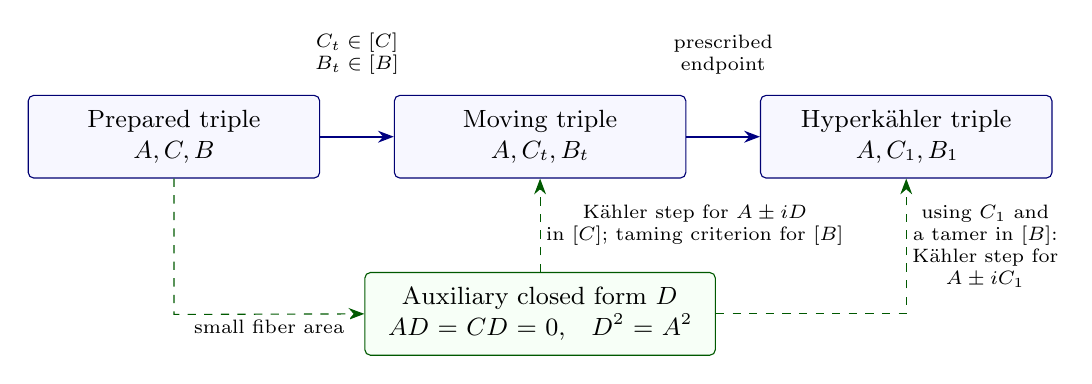
\begin{tikzpicture}[
  box/.style={draw=blue!45!black,rounded corners=2pt,
    fill=blue!3,align=center,text width=3.35cm,minimum height=1.05cm,
    inner sep=5pt,font=\small},
  aux/.style={box,draw=green!35!black,fill=green!3,text width=4.1cm},
  route/.style={-{Stealth[length=2mm]},thick,draw=blue!50!black},
  aid/.style={-{Stealth[length=2mm]},dashed,draw=green!35!black},
  lab/.style={font=\scriptsize,align=center,fill=white,inner sep=2pt}
]
\node[box] (start) at (0,0) {Prepared triple\\$A,C,B$};
\node[box] (move) at (4.65,0) {Moving triple\\$A,C_t,B_t$};
\node[box] (finish) at (9.3,0) {Hyperk\"ahler triple\\$A,C_1,B_1$};
\draw[route] (start) -- node[lab,above=20pt] {$C_t\in[C]$\\$B_t\in[B]$} (move);
\draw[route] (move) -- node[lab,above=20pt] {prescribed\\endpoint} (finish);
\node[aux] (auxiliary) at (4.65,-2.25)
  {Auxiliary closed form $D$\\$AD=CD=0$,\quad $D^2=A^2$};
\draw[aid] (start.south) -- ++(0,-1.725) --
  node[lab,below] {small fiber area} (auxiliary.west);
\draw[aid] (auxiliary.north) -- node[lab,right]
  {K\"ahler step for $A\pm iD$\\in $[C]$; taming criterion for $[B]$} (move.south);
\draw[aid] (auxiliary.east) -- (finish.south |- auxiliary.east) --
  node[lab,right] {using $C_1$ and\\a tamer in $[B]$:\\K\"ahler step for\\$A\pm iC_1$} (finish.south);
\end{tikzpicture}
\caption{The final deformation. Solid arrows trace the deformation; dashed
arrows indicate auxiliary dependencies. The upper row consists of
actual triples in the original classes. The auxiliary form supplies the
first integrable pair and the numerical control that keeps $[B]$
available along the moving pair. After both K\"ahler steps, the tamers
$B_t$ are chosen with initial value $B$ and final value $B_1$.}
\label{fig:endpoint-path}
\end{figure}


\begin{proof}[Proof of \Cref{thm:main}]
We trace the actual form paths and then construct the endpoint;
\Cref{fig:endpoint-path} summarizes the final stages.
All coefficient changes below are constant orthogonal changes, and
will be undone at the end.

\paragraph{\emph{The prepared pair.}}
Choose the primitive null class $F$ of \Cref{prop:chamber-class} and
rotate the coefficient basis so that $[B]$ points in the direction of
$F^+$ and the pair $[A],[C]$ spans its orthogonal plane in $P$.
The rotated initial triple is denoted $(A,C,B)$; its cohomology Gram
matrix is still the identity.

The families result and \Cref{prop:nonsplitting,thm:pencil} give an
exact pair deformation to a torus fibration with the stated standard
nodal neighborhoods, keeping $B$ fixed.
\Cref{prop:regular-preparation} then gives a further path of positive
closed triples to invariant regular data with the auxiliary form
$\Psi$.  Both stages preserve the three individual classes and start
at the actual representatives supplied by the preceding stage.
Retain the notation
$(A,C,B)$ for the resulting triple. In particular
\begin{equation}\label{eq:endpoint-periods}
 [A]^2=[C]^2=[B]^2=1,\qquad
 [A][C]=[A][B]=[C][B]=0.
\end{equation}

\paragraph{\emph{The auxiliary solution.}}
Fix a sufficiently small $\epsilon>0$ for
\Cref{thm:auxiliary-solution,prop:auxiliary-class}, and set
$D=D_\epsilon$. The form $D$ is closed and smooth and satisfies
\begin{equation}\label{eq:endpoint-auxiliary}
 AD=CD=0,\qquad D^2=A^2>0.
\end{equation}
The triple with forms $A,C,D$ is positive. The same choice of
$\epsilon$ gives the numerical conclusion of
\Cref{prop:auxiliary-class} for every later definite pair with the
classes $[A],[C]$. These choices precede the K\"ahler constructions
that follow.

\paragraph{\emph{The first K\"ahler step.}}
By \Cref{lem:complex-symplectic}, $A\pm iD$ is a nowhere-zero
holomorphic two-form for an integrable complex structure $I$; choose the
sign so that $C$ tames $I$. This is possible by
\Cref{lem:definite-pair} and positivity of $(A,D,C)$.
\Cref{prop:topology} gives even $b_1$, so the surface is K\"ahler.
The period relations \eqref{eq:endpoint-periods} and
\eqref{eq:endpoint-auxiliary} give
$[C][A]=[C][D]=0$. Therefore \Cref{lem:endpoint-hodge-type} puts
$[C]$ in real type $(1,1)$.

Apply \Cref{lem:endpoint-kahler-class} with
$H=[C]$ and $\nu=A^2$. Its integral condition holds by
\eqref{eq:endpoint-periods}. We obtain a K\"ahler representative
$C_1\in[C]$ satisfying
\begin{equation}\label{eq:endpoint-first-yau}
 AC_1=DC_1=0,\qquad C_1^2=A^2.
\end{equation}
Let $C_t=(1-t)C+tC_1$. Both endpoints tame $I$, so the entire segment
does. Thus $(A,D,C_t)$ is
positive, and $(A,C_t)$ is a definite pair in the original pair
classes. Moreover $D$ tames its associated almost-complex structure
with the continuously chosen sign. Indeed $D$ is wedge-orthogonal
to both pair forms by \eqref{eq:endpoint-auxiliary} and
\eqref{eq:endpoint-first-yau}, and has positive square.

\paragraph{\emph{Keeping the third class.}}
Let $J_t$ now denote the structure associated with the moving pair
$(A,C_t)$ and tamed by $D$. For every irreducible $J_t$ curve, its
class $d$ has $[D]d>0$. \Cref{prop:auxiliary-class} implies
$[B]d>0$, and places $[B]$ and $[D]$ in the same open timelike cone
of the fixed space $V$ from \eqref{eq:pair-lorentz-space}.
The hypotheses of \Cref{thm:taming-cone} therefore hold with
$U=[D]$ and $H=[B]$. Thus $[B]$ contains a tamer for every $J_t$.

At $t=0$ this sign of $J_t$ agrees with the sign previously tamed by
the actual third form $B$.  To check this pointwise, take a regular
fiber with its prepared orientation.  Both $B$ and $D$ restrict
positively to its tangent planes, which are complex lines for the
prepared pair.  They therefore select the same sign there.  On the
connected manifold $X$ this choice of sign cannot jump, so $B$ tames
$J_0$ everywhere.  We will choose the family of tamers after fixing its
final representative in the next step.

\paragraph{\emph{The second K\"ahler step.}}
The final pair $(A,C_1)$ is orthogonal with equal square by
\eqref{eq:endpoint-first-yau}.  Thus the structure $J_1$ already
selected by $D$ is integrable, with holomorphic volume form
$A\pm iC_1$ for the corresponding sign.  The preceding step supplies
a representative of $[B]$ taming this same $J_1$.  Even $b_1$ gives
K\"ahlerness again, and \eqref{eq:endpoint-periods} together with
\Cref{lem:endpoint-hodge-type} puts $[B]$ in type $(1,1)$.
Apply \Cref{lem:endpoint-kahler-class} with $H=[B]$ and $\nu=A^2$.
This yields a K\"ahler representative $B_1\in[B]$ such that
\begin{equation}\label{eq:endpoint-final-identities}
 AB_1=C_1B_1=0,\qquad B_1^2=A^2=C_1^2.
\end{equation}
Now apply \Cref{lem:smooth-tamers} to the family $J_t$, prescribing
the actual prepared form $B$ at $t=0$ and the newly constructed
$B_1$ at $t=1$.  It gives closed tamers $B_t\in[B]$ with these two
endpoint values.  Thus $(A,C_t,B_t)$ is a path of positive closed
triples in the original classes, joining the prepared triple to
$(A,C_1,B_1)$ itself.

Concatenate the finitely many triple paths, reparametrizing each to be
constant to all orders at its endpoints. This produces a smooth path
on $[0,1]$. Each component is closed and remains in its original
class, and positivity holds at every parameter. By
\eqref{eq:endpoint-first-yau} and
\eqref{eq:endpoint-final-identities}, if
$(\eta_1,\eta_2,\eta_3)=(A,C_1,B_1)$ and $\mu_1=A^2/2$, then
\[
 \eta_i\wedge\eta_j=2\delta_{ij}\mu_1.
\]
By \Cref{lem:complex-symplectic}, these forms are parallel and
self-dual for a hyperk\"ahler metric with volume $\mu_1$.
Finally undo the initial orthogonal change of coefficients.
Orthogonality preserves the displayed identity and restores the
original ordered classes, proving the theorem.
\end{proof}

\bibliographystyle{amsplain}
\bibliography{references}
\end{document}
